%----------------------------------------------------------------------------------------
%	PACKAGES AND OTHER DOCUMENT CONFIGURATIONS
%----------------------------------------------------------------------------------------


\documentclass[11pt, a4paper, oneside]{Thesis} % Paper size, default font size and one-sided paper

\graphicspath{{./Pictures/}} % Specifies the directory where pictures are stored

\usepackage[square, numbers, comma, sort&compress]{natbib} % Use the natbib reference package - read up on this to edit the reference style; if you want text (e.g. Smith et al., 2012) for the in-text references (instead of numbers), remove 'numbers' 
\hypersetup{urlcolor=black, colorlinks=true} % Colors hyperlinks in blue - change to black if annoying
\title{\ttitle} % Defines the thesis title - don't touch this

\usepackage{tikz}
\usepackage{setspace}

\definecolor{OrangeGSSI}{RGB}{237,113,45}
\definecolor{blue}{RGB}{25,25,112}

%----------------------------------------------------------------------------------------
%	DOCUMENT VARIABLES
%	Fill in the lines below to update the thesis template
%	If you wish to cite each of the variables defined below, look at the
%	section above for the citation command e.g. \examiner{} below is
%	defined as \examname above so you cite it as \examname
%----------------------------------------------------------------------------------------

\thesistitle{Adaptive Influence Maximization: Bounding Adaptivity Gaps and Beyond} % Your thesis title - this is used in the title and abstract
%-------------------------------------------------  
\supervisor{Prof. Gianlorenzo \textsc{D'Angelo}\\ Dr. Cosimo \textsc{Vinci}}% You supervisor's name - this is used in the title page
%-------------------------------------------------   



\examiner{Dr. Name  \textsc{Surname}} % Your examiner's name - this is not currently used anywhere in the template, cite it with \examname if you want it
%-------------------------------------------------   
\degree{Doctor of Philosophy} % Your degree name - this is currently used in the title page and abstract
%-------------------------------------------------   
\authors{Debashmita \textsc{Poddar}} % Your name - this is used in the title page and abstract
%-------------------------------------------------

%----------------------------------------------------------------------------------------
%	TYPESETTING
%----------------------------------------------------------------------------------------
%\usepackage{algorithm}
\usepackage{algorithmic}
\usepackage{pifont}
\usepackage{xcolor,colortbl}
\usepackage{flushend}
\usepackage[normalem]{ulem} % for \sout
\usepackage{multicol}
\usepackage{adjustbox}
\usepackage{xcolor}
\usepackage{tabularx,booktabs,caption,ragged2e}
\newcommand{\ugh}[1]{\textcolor{red}{\uwave{#1}}} % please rephrase
\newcommand{\ins}[1]{\textcolor{blue}{\uline{#1}}} % please insert
\newcommand{\del}[1]{\textcolor{red}{\sout{#1}}} % please delete
\newcommand{\chg}[2]{\textcolor{red}{\sout{#1}}{\ra}\textcolor{blue}{\uline{#2}}} % please change

\renewcommand{\ttdefault}{cmr}

\newcommand{\assignedto}[1]{\textcolor{red}{\ding{46}~{\sf Assigned to:}~#1}\\}
\newcommand{\todo}[1]{\textcolor{blue}{\ding{46}{\sf}~#1}}

\newcommand{\sugg}[1]{\textcolor{orange}{#1}}
%----------------------------------------------------------------------------------------
%	End of TYPESETTING
%----------------------------------------------------------------------------------------

\begin{document}

\frontmatter % Use roman page numbering style (i, ii, iii, iv...) for the pre-content pages

\setstretch{1.3} % Line spacing of 1.3

% Define the page headers using the FancyHdr package and set up for one-sided printing
\fancyhead{} % Clears all page headers and footers
\rhead{\thepage} % Sets the right side header to show the page number
\lhead{} % Clears the left side page header

% \pagestyle{fancy} % Finally, use the "fancy" page style to implement the FancyHdr headers
\newcommand{\HRule}{\rule{\linewidth}{0.5mm}} % New command to make the lines in the title page

% PDF meta-data
\hypersetup{pdftitle={\ttitle}}
\hypersetup{pdfsubject=\subjectname}
\hypersetup{pdfauthor=\authornames}
\hypersetup{pdfkeywords=\keywordnames}

%----------------------------------------------------------------------------------------
%	TITLE PAGE
%----------------------------------------------------------------------------------------

\begin{titlepage}
\begin{center}


\includegraphics[width=0.4\textwidth]{./figures/logo_GSSI}~\\[1cm]
\textsc{\Large PhD Thesis}\\[0.5cm] % Thesis type

\HRule \\[0.1cm] % Horizontal line
{\huge \bfseries Adaptive Influence Maximization: \\[0.3cm] Bounding Adaptivity Gaps and Beyond}\\[0.3cm] % Thesis title
\HRule \\[0.9cm] % Horizontal line

{\Large \textsc{PhD Program in Computer Science: XXXIV cycle}}\\[2cm]

\begin{minipage}{0.4\textwidth}
\begin{flushleft} \large
\emph{Author:}\\
\bigskip \authornames \\
\href{mailto:debashmita.poddar@gssi.it}{debashmita.poddar@gssi.it}
%\href{http://www.johnsmith.com}{\authornames} % Author name - remove the \href bracket to remove the link
\end{flushleft}
\end{minipage}
\begin{minipage}{0.5\textwidth}
\begin{flushright} \large
\emph{Supervisors:} \\
%\href{http://www.jamessmith.com}{\supname} % Supervisor name - remove the \href bracket to remove the link  
\bigskip \supname \\
\href{mailto:gianlorenzo.dangelo@gssi.it}{gianlorenzo.dangelo@gssi.it\\ cosimo.vinci@unisalento.it} \\
%\bigskip \bigskip
%\emph{Internal advisor:} \\
%\bigskip \examname \\
%\href{mailto:name.surname@gssi.infn.it}{name.surname@gssi.infn.it}
\end{flushright}
\end{minipage}\\[2.2cm]
 
%\large \textit{A thesis submitted in fulfilment of the requirements\\ for the degree of \degreename}\\[0.3cm] % University requirement text
%\textit{in the}\\[0.4cm]
%\groupname\\\deptname\\[2cm] % Research group name and department name


{\large \today}\\[2.2cm] % Date

\univname \\
\addressnames
%\includegraphics{Logo} % University/department logo - uncomment to place it
 
\vfill
\end{center}
\afterpage{\blankpage}
\end{titlepage}


%----------------------------------------------------------------------------------------
%	DECLARATION PAGE
%	Your institution may give you a different text to place here
%----------------------------------------------------------------------------------------

%\Declaration{
%
%\addtocontents{toc}{\vspace{1em}} % Add a gap in the Contents, for aesthetics
%
%I, \authornames, declare that this thesis titled, '\ttitle' and the work presented in it are my own. I confirm that:
%
%\begin{itemize} 
%\item[\tiny{$\blacksquare$}] This work was done wholly or mainly while in candidature for a research degree at this University.
%\item[\tiny{$\blacksquare$}] Where any part of this thesis has previously been submitted for a degree or any other qualification at this University or any other institution, this has been clearly stated.
%\item[\tiny{$\blacksquare$}] Where I have consulted the published work of others, this is always clearly attributed.
%\item[\tiny{$\blacksquare$}] Where I have quoted from the work of others, the source is always given. With the exception of such quotations, this thesis is entirely my own work.
%\item[\tiny{$\blacksquare$}] I have acknowledged all main sources of help.
%\item[\tiny{$\blacksquare$}] Where the thesis is based on work done by myself jointly with others, I have made clear exactly what was done by others and what I have contributed myself.\\
%\end{itemize}
% 
%Signed:\\
%\rule[1em]{25em}{0.5pt} % This prints a line for the signature
% 
%Date:\\
%\rule[1em]{25em}{0.5pt} % This prints a line to write the date
%}
%
%\clearpage % Start a new page

%----------------------------------------------------------------------------------------
%	QUOTATION PAGE
%----------------------------------------------------------------------------------------

%\pagestyle{empty} % No headers or footers for the following pages
%
%\null\vfill % Add some space to move the quote down the page a bit
%
%\textit{``Thanks to my solid academic training, today I can write hundreds of words on virtually any topic without possessing a shred of information, which is how I got a good job in journalism."}
%
%\begin{flushright}
%Dave Barry
%\end{flushright}
%
%\vfill\vfill\vfill\vfill\vfill\vfill\null % Add some space at the bottom to position the quote just right
%
%\clearpage % Start a new page

%----------------------------------------------------------------------------------------
%	ABSTRACT PAGE
%----------------------------------------------------------------------------------------
\afterpage{\blankpage}

\addtotoc{Abstract} % Add the "Abstract" page entry to the Contents

\abstract % Add a gap in the Contents, for aesthetics

The \textit{influence maximization (IM)} problem is a discrete optimization problem [Kempe et al.~\cite{Kempe2003}] of selecting the $k$ most influential nodes in a network, and has ample applications ranging from viral marketing to outbreak detection. The IM problem is as follows: given a budget $k$ and a graph $G$, our goal is to find a seed set $S$ consisting of $k$ nodes of $G$ which maximizes the expected number of nodes influenced by $S$, according to some model of influence diffusion. The classic IM problem, which is also referred to as the \textit{non-adaptive IM}, selects the seed set $S$ before starting the diffusion process. Therefore, the focus is on the efficiency of the solution.

A few years later, Golovin and Krause~\cite{Golovin2011a} introduced the \textit{adaptive IM (AIM)} to target the efficacy of the problem. In the adaptive setting, selection of the $k$ seed nodes occurs one at a time, such that the $j$-th seed node is selected after observing the actual influence from the previously selected $j-1$ seeds. There are two main feedback models that have been studied: \textit{full-adoption}, where the entire diffusion carried out by a seed node in the previous step is observed, and \textit{myopic}, where only the neighbours of the previously selected seed nodes are considered as a feedback.

While adaptive policies are strictly stronger than non-adaptive ones, the latter are much easier to design and implement. Golovin and Krause~\cite{Golovin2011a} proposed a measure called the \textit{adaptivity gap (AG)}, which is the ratio between the adaptive and non-adaptive optima. If the AG is small, we say that the non-adaptive policy provides a good approximation of the adaptive optimum.

In this thesis, we study AG with both feedback models. Under the full adoption feedback, we investigate the upper bound of AG over several graph classes, from in-arborescences to general graphs. We show the first sub-linear upper bound on AG that holds for any graph. 
Next, we have the experimental part, where we take different network models, such as random, scale-free and real world networks, and draw several comparisons between the adaptive greedy and the non-adaptive greedy algorithms under various network settings and parameters.

Eventually, we move on to the myopic feedback model, which lacks the property of submodularity. To recover from the drawbacks of being non-submodular, an artificial diffusion process is taken into account. We introduce a new technique to bound the AG without using the commonly used approaches, such as multi-linear extensions or random walks. We also study the adaptive greedy algorithm under the new setting and compare it to optimal adaptive policy. Our approach is of independent interest and can be used for further studies related to  different adaptive optimization problems.




\clearpage % Start a new page

%----------------------------------------------------------------------------------------
%	ACKNOWLEDGEMENTS
%----------------------------------------------------------------------------------------

\setstretch{1.3} % Reset the line-spacing to 1.3 for body text (if it has changed)

\acknowledgements{\addtocontents{toc}{\vspace{1em}} % Add a gap in the Contents, for aesthetics

I thank my supervisors for being a positive influence in both academia and my life in particular. Prof. Gianlorenzo D'Angelo, for being a patient and kind person. Gianlorenzo's pursuit of high standards in research have deeply shaped and impressed me over the years. He has invariably given me feedback on my work in the most benevolent way as possible. 
Dr. Cosimo Vinci as a forbearing supervisor, for consistently teaching and answering my questions without a speck of annoyance on his face. His unlimited enthusiasm in every aspect has motivated me to stick to this PhD during the bleaker times. Gianlorenzo and Cosimo always checked on my overall health before talking about work, and I am grateful for that.

My parents, for always letting me follow my dreams and being the pillars of strength. \textit{Baba}, you really made me a strong and independent woman to deal with the world through your unusual ways. \textit{Ma}, thank you for educating me to look beyond the appearance and have empathy.

My grandparents, who were amazing, and loved me till their last breath. I give them most of the credits for making me a good human being. There were times when I had to question my moral and their teachings reminded me of who I am. I miss them both, even though I don't talk about it often.

Pritom and Saili for being my only strand of family in Europe. I have spent most of the Christmas holidays in the course of my PhD with them, eating the delectable food Saili made for us. Thank you, brother, for always keeping me entertained, during the stressful periods.

Théo, for truly being my best friend and always believing in me with complete honesty. You have been an incredibly supportive and dedicated \textit{ami} during the last seven and a half years I have known you. \textit{Merci}!

A handful of people at the GSSI whom I call my adulting friends. These people have taken up the baton to teach me a lot of valuable life lessons. My heartfelt thanks to the entire GSSI community and the CS department for doing what they do the best.

Last but not the least, \textit{grazie mille} to the \textit{bella città} of L'Aquila, and the nice people I have encountered during these four years. Waking up to the beautiful view of the mountains definitely did good to my soul and helped me endure the shortcomings. Also, there is no better place than L'Aquila to learn about the Italian bureaucracy. This has been my second challenge, other than research, and there remains to be a lot of open problems which has been verified by many in the same boat as me.



}
\clearpage % Start a new page

\afterpage{\blankpage}
%----------------------------------------------------------------------------------------
%	LIST OF CONTENTS/FIGURES/TABLES PAGES
%----------------------------------------------------------------------------------------



\pagestyle{fancy} % The page style headers have been "empty" all this time, now use the "fancy" headers as defined before to bring them back

\lhead{\emph{Contents}} % Set the left side page header to "Contents"
\tableofcontents % Write out the Table of Contents

\lhead{\emph{List of Figures}} % Set the left side page header to "List of Figures"
\listoffigures % Write out the List of Figures

\lhead{\emph{List of Tables}} % Set the left side page header to "List of Tables"
\listoftables % Write out the List of Tables

\afterpage{\blankpage}

%%----------------------------------------------------------------------------------------
%%	ABBREVIATIONS
%%----------------------------------------------------------------------------------------
%\clearpage % Start a new page
%\setstretch{1.5} % Set the line spacing to 1.5, this makes the following tables easier to read
%\lhead{\emph{Abbreviations}} % Set the left side page header to "Abbreviations"
%\listofsymbols{ll} % Include a list of Abbreviations (a table of two columns)
%{
%\textbf{AMI} & \textbf{A}dvanced \textbf{M}etering \textbf{I}nfrastructure \\
%\textbf{CPS} & \textbf{C}yber-\textbf{P}hysical \textbf{S}ystems \\
%\textbf{DoS} & \textbf{D}enial-\textbf{o}f-\textbf{S}ervice \\
%\textbf{MAC} & \textbf{M}edium \textbf{A}ccess {C}ontrol \\
%\textbf{MAPE} & \textbf{M}onitor, \textbf{A}nalyse, \textbf{P}lan, \textbf{E}xecute \\
%\textbf{MCN} & \textbf{M}ulti-hop \textbf{C}ontrol \textbf{N}etwork \\
%\textbf{MILS} & \textbf{M}ultiple \textbf{I}ndependent \textbf{L}evels of \textbf{S}ecurity/Safety\\
%\textbf{MRMC} & \textbf{M}arkov \textbf{R}eward \textbf{M}odel \textbf{C}hecker \\
%\textbf{MTD} & \textbf{M}oving \textbf{T}arget \textbf{D}efence \\
%\textbf{NICS} & \textbf{N}etworked \textbf{I}ndustrial \textbf{C}ontrol \textbf{S}ystems \\
%\textbf{OPC} & \textbf{O}bject linking and embedding for \textbf{P}rocess \textbf{C}ontrol \\
%\textbf{PCS} & \textbf{P}rocess \textbf{C}ontrol \textbf{S}ystems \\
%\textbf{PLC} & \textbf{P}rogrammable \textbf{L}ogic \textbf{C}ontroller \\
%\textbf{PRISM} & \textbf{P}robabilistic \textbf{S}ymbolic \textbf{M}odel \textbf{C}hecker \\
%\textbf{RTU} & \textbf{R}emote \textbf{T}erminal \textbf{U}nit \\
%\textbf{SCADA} & \textbf{S}upervisory \textbf{C}ontrol \textbf{A}nd \textbf{D}ata \textbf{A}cquisition\\
%\textbf{SLR} & \textbf{S}ystematic \textbf{L}iterature \textbf{R}eview \\
%\textbf{SMC} & \textbf{S}tatistical \textbf{M}odel \textbf{C}hecking \\
%\textbf{VCSE} & \textbf{V}irtual \textbf{C}ontrol \textbf{S}ystem \textbf{E}nvironment \\
%%\textbf{Acronym} & \textbf{W}hat (it) \textbf{S}tands \textbf{F}or \\
%}

%----------------------------------------------------------------------------------------
%	PHYSICAL CONSTANTS/OTHER DEFINITIONS
%----------------------------------------------------------------------------------------

%\clearpage % Start a new page
%
%\lhead{\emph{Physical Constants}} % Set the left side page header to "Physical Constants"
%
%\listofconstants{lrcl} % Include a list of Physical Constants (a four column table)
%{
%Speed of Light & $c$ & $=$ & $2.997\ 924\ 58\times10^{8}\ \mbox{ms}^{-\mbox{s}}$ (exact)\\
%% Constant Name & Symbol & = & Constant Value (with units) \\
%}

%----------------------------------------------------------------------------------------
%	SYMBOLS
%----------------------------------------------------------------------------------------

%\clearpage % Start a new page
%
%\lhead{\emph{Symbols}} % Set the left side page header to "Symbols"
%
%\listofnomenclature{lll} % Include a list of Symbols (a three column table)
%{
%$a$ & distance & m \\
%$P$ & power & W (Js$^{-1}$) \\
%% Symbol & Name & Unit \\
%
%& & \\ % Gap to separate the Roman symbols from the Greek
%
%$\omega$ & angular frequency & rads$^{-1}$ \\
%% Symbol & Name & Unit \\
%}

%----------------------------------------------------------------------------------------
%	DEDICATION
%----------------------------------------------------------------------------------------

\setstretch{1.3} % Return the line spacing back to 1.3
%
%\pagestyle{empty} % Page style needs to be empty for this page
%
%\dedicatory{For/Dedicated to/To my\ldots} % Dedication text
%
%\addtocontents{toc}{\vspace{2em}} % Add a gap in the Contents, for aesthetics

%----------------------------------------------------------------------------------------
%	THESIS CONTENT - CHAPTERS
%----------------------------------------------------------------------------------------

\mainmatter % Begin numeric (1,2,3...) page numbering

\pagestyle{fancy} % Return the page headers back to the "fancy" style

% Include the chapters of the thesis as separate files from the Chapters folder
% Uncomment the lines as you write the chapters
\fancyhead{}
\rhead{\thepage}
 \setcounter{page}{1}
%----------------------------------------------------------------------------------------
%	Introduction
%----------------------------------------------------------------------------------------



\chapter{Introduction}\label{chap:intro}
\fancyhead[L]{\textit{Chapter 1. Introduction}}


{\textit{``To develop a complete mind: Study the science of art; Study the art of science. Learn how to see. Realize that everything connects to everything else."}}

\rightline{--- Leonardo Da Vinci}




\section{How connected are real world networks?} \label{sec:work}

Stanley Milgram in his classic paper, \emph{The Small-World Problem} \cite{milgram}, put forth the notion of transitive dependency among people in a social network. He states that when a person, named Bob, is connected by a series of links to another person, called Alice, there are, on average, five intermediate people between Bob and Alice. 
Brown and Reingen \cite{brown} studied real networks and found the importance of stronger and weaker links associated with recommendation systems. Stronger links are seen as a measure of reliability for a certain recommendation, whereas weaker links are associated with the traversal of information from one cluster to another playing an important role in the networking ecosystem.


Social networking sites have seen a significant boom in the past two decades. These sites play a crucial role in spreading new ideas or innovations through its fundamental network structure consisting of individuals and their relationship with other individuals. Major networking sites with over a hundred million active users include \emph{Facebook, Twitter, Instagram}, etc. In other words, \emph{social networks} are a collection of \emph{entities} which form \emph{relationships} with other entities participating in the same network. 


Due to the increase of information propagation in the networking sites, networks have become increasingly complex. Researchers have been trying to decode the properties and patterns exhibited by such massive networks. \emph{Social Network Analysis (SNA)} has emerged as the study of social networks using \emph{collaboration graphs}, in which the entities are modelled by the nodes of a graph and the relationship between the entities are modelled by a set of edges. Formally, a \emph{Social Graph} $G = (V, E)$ is a directed graph (sometimes undirected), where \emph{V} is the set of nodes representing the entities of the network, and $E$ is the set of edges  representing the relationship existing between those entities. SNA is the field of study at the intersection between \emph{Graph Theory, Networking} and \emph{Sociology}.



\section{Application of social networks: Viral Marketing}

\emph{Marketing} is the promotion of a product by a company to its customer base. It takes into account the \emph{word-of-mouth} effect, i.e., a customer who has used the products, can recommend it to her friends. \emph{Viral Marketing (VM)} supports the same theory, and uses social networks as a platform for recommendations. The method follows the principle of contiguous viruses: if the flu infects one person, any person who comes in contact with the infected person also catches the flu with high probability.

In social networks, the company distributes some free or discounted products to specific individuals who are capable of marketing it. These individuals may recommend it to their neighbours after using it, who in turn might recommend it to their neighbours, and so on, following an iterative diffusion process. The direct analogy to this is \emph{Influencer Marketing}. Influencers are those particular individuals in the network, who have a significant number of followers in a specific niche, and can affect the decisions of the people following her. Companies who want to launch new products in the market generally offer their products to the influencers, particularly to those who are closer to the specific customer base for selling the considered products. 

Krackhardt et al.~\cite{Iacobucci2014} states that a marketer can leverage her sales profit by knowing the topology of the underlying social network. They also introduced the concept of distributing free products to the influencers. Domingos and Richardson~\cite{Domingos2001,Richardson2002} introduce some models of viral marketing, and raise the following algorithmic question: \textit{in a vast connected network, if a seller markets a product, how should they choose a set of influential buyers (nodes) who can reach out to (influence) as many nodes as possible to buy that product?} Indeed, the number of such buyers are directly proportional to the seller's profit. Kempe et al.~\cite{Kempe2003,kempe05,Kempe2015}, in their seminal works, presented VM as a discrete optimization problem, and called it the \emph{influence maximization (IM)} problem, discussed in details in the upcoming sections and chapters.      

\section{From viral marketing towards maximizing influence in networks}

The IM problem as described by Kempe et al.~\cite{Kempe2003} is an one-shot task: given a static social network $G$, a diffusion model with given parameters, select the seed set $S$, and with only one propagation pass through the entire network, $S$ activates $k$ nodes, with the expectation of maximizing the number of active nodes in the network. 


The utility function, $f$, which needs to be maximized is shown to be submodular ($f$ satisfies the ``diminishing returns" property) and  monotone (number of active nodes either increase or remain the same). Since the problem is NP-hard by nature (shown by reduction through \textit{Set Cover Problem}), approximation algorithms needs to be used. From the results of Nemhauser et al.~\cite{Company1978, nemhauser}, Kempe et al.~\cite{Kempe2003} showed that the results obtained from a simple greedy algorithm will reach at least $(1-1/e)$ of the optimal solution.


\subsection*{Independent Cascade (IC) Model}

Goldenberg et al.~\cite{J.2001}, Goldberg and Liu \cite{Goldberg2013} used the concept of \emph{Cellular Automata} as a framework to model the diffusion of information in the network. The \emph{Independent Cascade(IC)} model, named by Kempe et al.~\cite{Kempe2003} models the dynamics of the viral marketing scenario and draws inspiration from the field of interacting particle systems. Initially, the diffusion model starts with a set of active nodes $S$ such that $|S| \leq k$. Each edge $e=(u,v)\in E$, has an influence probability $p_{uv}$ attached to it, so that node $u$ will activate node $v$ with a probability $p_{uv}$, independently from the other nodes. 

With the above parameters as input to the system, the diffusion process unravels in several time steps. At time step $t$, if node $u$ is active, it is given a single opportunity to activate its neighbour $v$ with probability $p_{uv}$. If node $v$ becomes active at time step $t$, it will further attempt to activate its neighbours at time step $t+1$ according to the influence probability. The process iteratively continues and comes to a halt when there are no more activations. Since the diffusion process spreads in a cascading manner, and each activation is independent from the other, the model is named as the independent cascade model.


\paragraph*{Linear Threshold (LT).} Differently from the IC model, where each activation is independent from each other, the LT model follows a more complex contagion process. Each node $v$ is  associated with a threshold value $\theta_v$, and to activate $v$, the probability associated with the  active edges from $v$'s neighbours need to cross the threshold $\theta_v$. This model is not in the scope of the thesis except for the experimental part in Chapter \ref{chap:background}. However, in Chapter \ref{chap:lit}, Section \ref{sec:lt} we will discuss the technical part of the LT model. 

\subsection*{Adaptive Influence Maximization}

In the \emph{Adaptive Influence Maximization (AIM)} \cite{Golovin2011}, we consider the adaptive version of the IC model. An adaptive policy $\pi$ is a function associating the {\em network state} with a new node that should be added to the seed set $S$, where the network state is what a policy observes at each time. The function $f$ that we want to maximize in expectation is the number of nodes that are reached by the spread of information.

The AIM problem wants to find a policy with a seed-set maximizing the expected value of $f$ (according to the probability distribution of the realizations), where the cardinality of the seed set must be at most $k$. The seed nodes are selected in multiple time steps, based on the observations or feedback obtained from the previous steps. The quality of seed nodes selected under the adaptive setting is better and also the influence generated is further improved because of the feedback provided by the network.




\subsection*{Feedback models}

There are two commonly used feedback models: \textit{full adoption} and \textit{myopic}. A full adoption feedback model records the entire spread generated by a seed node. The adaptive policy $\pi$ observes this feedback and then decides on the selection of the next seed node. As mentioned before, the underlying diffusion model considered in this thesis is the independent cascade model, which is adaptive submodular and monotone for the full adoption feedback~\cite{Golovin2011a}. Golovin and Krause~\cite{Golovin2011a} exploited the desired adaptive submodularity property of the objective function $f$, and applied the results from Nemhauser et al.~\cite{nemhauser,Company1978} to show that the solution provided by an adaptive greedy policy is at least $(1-1/e)$ of the optimal adaptive policy.

The myopic feedback model observes the current state of a seed node's immediate neighbours only. This model is shown to be adaptive non-submodular by nature in \cite{Golovin2011}. In order to evaluate the performance of this model, we need to recover the adaptive submodularity via an artificial diffusion model, which gives a seed node multiple chances to activate its neighbours \cite{Chen2019, DAngeloPV21}. The feedback models will be discussed later at length in Section \ref{feedback}.

\subsection*{Adaptivity Gap}

Another important term coined by Golovin and Krause~\cite{Golovin2011a} is the \emph{Adaptivity Gap (AG)}. The AG quantifies how well does an optimal non-adaptive policy, that is a policy in which all the edges should be selected at beginning, without observing the realization, perform when compared to an optimal adaptive policy. To measure the efficiency of a non-adaptive greedy algorithm, we can multiply the adaptivity gap with the approximation factor to compare the performance ratio of the algorithm with the optimal adaptive policy.



\section{Necessity to bound the Adaptivity Gap} \label{sec:ag}

Due to the feedback received after every round of seed selection, the efficiency in terms of time reduces for an adaptive policy. However, a non-adaptive policy is a straightforward simple process, and the overhead in time is negligible compared to the adaptive policies. 
Also, a non-adaptive algorithm is much simpler to design since the seed selection takes place in the beginning of the diffusion process, and we do not keep track of the nodes that are activated at each time step. 

 
\begin{figure}
\centering
    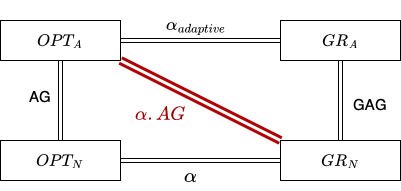
\includegraphics[width=0.7\linewidth]{GSSI_thesisProposal/figures/AG.png}
    \caption{Connection between optimal and greedy policies.}
\label{fig:ag}
\end{figure}

The adaptivity gap gives us the ratio to check how efficient the seed set selected by the optimal non-adaptive policy is compared to the adaptive optimal over different graph classes. A tighter bound is preferred, but the main challenge is to find an upper bound that is closer to 1, which will indicate that there exists an optimal non-adaptive policy that is as efficient as the optimal adaptive policy for that graph class. 
The thesis tries to find and then improve on these upper bounds on the different graph classes using newer techniques and by studying the ones that are used in the past. 

In Section \ref{exp} we will encounter the efficiency of the adaptive greedy algorithm based on the memory consumption. With a faster best estimate, the non-adaptive greedy policy tends to consume a huge part of the memory as the size of the graph grows, hence asking for better memory management. A non-adaptive greedy algorithm is generally preferred over an adaptive one due to the above stated reasons, and hence a measure is needed to calculate the efficiency of such algorithms. Another measure called the \emph{greedy adaptivity gap (GAG)} \cite{Chen2019a}, which measures the generated spread  between the greedy adaptive algorithm and the greedy non-adaptive algorithm, helps us to navigate through the performance efficiency of a non-adaptive greedy algorithm over a adaptive greedy one. Figure \ref{fig:ag} depicts the ratio between the optimals and the greedy algorithms (refer to table \ref{sec:not} for the notations used in the figure). The diagonal red line is the most important factor to bound, since it directly estimates by how much an optimal adaptive strategy outperforms a non-adaptive greedy algorithm, and helps us to design better algorithms by having an optimal measure in mind. 


\section{Contributions} \label{sec:cont}

\begin{enumerate}


    \item  \textit{Gianlorenzo D’Angelo, Debashmita Poddar, and Cosimo Vinci ``Better bounds on the adaptivity gap of influence maximization under full-adoption feedback", Thirty-Fifth AAAI Conference on Artificial Intelligence, AAAI, 2021.}

    The extended version of the above paper is accepted at the \textit{Artificial Intelligence Journal (AIJ)} \cite{AIJ}.

\paragraph{Full-adoption feedback.}


 

Chapter \ref{chap:background} is mainly related to the results obtained in the aforementioned paper (that is, \cite{DAngelo}), in which we conduct an extensive study on the full adaption feedback model under IC. 
First, we tackle the in-arborescences, which were already studied by \cite{Chen2019} in the adaptive setting. Chen and Peng \cite{Chen2019} derived an upper bound on adaptivity gaps using Poisson process and multi-linear extensions. We bypass those techniques and give a simpler and quicker solution to connect the non-adaptive and adaptive optimals. Eliminating the techniques used by \cite{Chen2019} and building the proof on the marginals related to the hybrid non-adaptive policy reduces the upper bound on adaptivity gap for the in-arborescences from 3.16 to 2.31 (Section \ref{sec_inarb}).

We further exploit our technique, to arrive at the first ever sub-linear upper bound on general graphs. To the best of our knowledge, this is the first and only bound known for general graphs with this setting. We show that under the Independent Cascade model with a full adoption feedback, the adaptivity gap of general graphs is $\lceil n^{1/3}\rceil$, where $n$ is the number of nodes in the graph (Section \ref{sec_gen}).

Next, we derive results on more specific graphs such as the $\alpha$-bounded graphs that includes several undirected graph topologies like a star, cycle, clique (with more than 3 nodes), etc. The $\alpha$-bounded graphs are undirected graphs where for nodes more than degree 2, their degree summation is at most $\alpha$. We show that the adaptivity gap for such bounded graphs is $\sqrt{\alpha}+O(1)$ and for 0-bounded graphs we get 3.16 as the upper bound (Section \ref{sec_alpha}).

We also address a very interesting class of graphs called the $(\beta,\gamma)$-bounded-activation graphs which denotes a cluster of graphs where the nodes that have at most $\gamma$ neighbours have $\beta$ influence in expectation. For $k \geq 2$, the adaptivity gap for such influence graphs is $\sqrt{\beta}+\frac{1}{1-\gamma}$ (Section \ref{sec:beta}).

The chapter is concluded by a series of experiments (Section \ref{exp}) on a bunch of well known networks (generated), that simulate the network (Erdős-Rényi,Watts-Strogatz and Barabási-Albert) and a real world Facebook network. This part includes new results that have not yet been published, and shows how a state-of-the-art non-adaptive greedy algorithm ($TIM^+$) performs when compared to its adaptive counterpart, which has the same underlying code as the non-adaptive greedy. We observe that the greedy adaptivity gap, which is the ratio between the adaptive greedy spread and the non-adaptive greedy, is closer to one for almost all the different network settings. This directly implies that the greedy non-adaptive algorithm ($TIM^+)$ used here, has an efficiency rate close to that of a greedy adaptive algorithm.




 
 \item  \textit{Gianlorenzo D’Angelo, Debashmita Poddar, and Cosimo Vinci ``Improved approximation factor for adaptive influence maximization via simple greedy strategies", 48th International Colloquium on Automata, Languages, and Programming, ICALP, 2021.}



\paragraph{Myopic feedback.} 


Chapter \ref{chap:sota} represents the aforementioned work (that is, \cite{DAngeloPV21}) which improves on \cite{Chen2019a}. The main difficulty faced with the myopic model is the lack of adaptive submodularity. This drawback makes the model non-trivial to analyze and hence we resort to an artificial model called the 2-level diffusion model. We use a similar concept introduced by \cite{Chen2019a}, where the seed node gets multiple chances to activate its neighbours. However, instead of using random walks on optimal decision trees and multilinear extension like in \cite{Chen2019a}, we directly analyze the non-adaptive greedy algorithm and relate it to an optimal adaptive solution which in turn improves the upper bound on the adaptivity gap from 4 to 3.164.

This flexibility of not passing through the adaptivity gap, gives us a more direct and improved approximation factor for both the non-adaptive greedy algorithm and the adaptive greedy. For achieving the approximation ratio for non-adaptive greedy algorithm we resort to a randomized non-adaptive policy to relate the expected spread of the non-adaptive greedy with the adaptive policy and arrive at 0.316, which is an improvement from 0.158 (Section \ref{sec_nag}).

The approximation factor for the adaptive greedy algorithm is found in a similar fashion by introducing the strong 2-level diffusion model and a strong 2-level hybrid policy. The difference with the above mentioned policy lies in the fact that the strong hybrid policy is conditioned by the partial realisations, which is not the case in the simple hybrid adaptive policy. The approximation factor is bounded by 0.393 for the adaptive greedy (Section \ref{ad-sec}).
\end{enumerate}

\section {Organization of the Thesis} \label{sec:org}
This thesis approaches on bounding the adaptivity gap using different techniques, and elucidates on the feedback models with different graph classes. The underlying diffusion model considered here is the independent cascade model and a part of the experiment is conducted on linear threshold.

\begin{itemize}

    \item \textit{Chapter \ref{chap:intro}} gives a general overview of the contents of this thesis and gives a high-level introduction on the topics that will be tackled here. A table of notations is provided to ease the access of all the symbols that will be used throughout the thesis.
    
    \item \textit{Chapter \ref{chap:lit}} carries out an in-depth analysis of the IM problem with the different diffusion models. The chapter continues to provide further details on the AIM problem, an exhaustive analysis of the feedback models and their adaptivity gaps. Furthermore, the chapter navigates through the related state-of-the-art research that has been conducted in this field. 
    
    \item \textit{Chapter \ref{chap:background}} studies the full-adoption feedback under the IC model with different graph classes (in-arborescences, general graphs, $\alpha$-bounded-degree graphs, $(\beta,\gamma)$-bounded-activation graphs). The chapter contains new techniques and the corresponding results on the upper bound of the AG related to the above mentioned graphs. The last part of the chapter deals with experiments which is important to uncover the efficiency of the greedy algorithms with different networks and parameters, giving us a further insight of the complexity to bound both the adaptivity gap and the greedy adaptivity gap.
    
    \item \textit{Chapter \ref{chap:sota}} contains the results related to the infamous adaptive non-submodular myopic feedback model with IC and explores a new way of reducing the upper bound on AG. The chapter also explores the greedy algorithms to achieve better approximations on the adaptive greedy and the non-adaptive greedy algorithms.
    
    \item \textit{Chapter \ref{chap:proposal}} concludes the thesis by summarizing the main results obtained during the PhD. There is a dedicated section related to some application of the graph classes and feedback models studied in the thesis to motivate further research on this topic. Lastly, we discuss the open problems that can be tackled in the future by referring to the works conducted in this PhD thesis. 
    \end{itemize}

\pagebreak

\section{Table of Notations} \label{sec:not}

    \begin{table} [ht]
    \centering
    \caption{Table of Notations}
    \begin{adjustbox}{width=1\textwidth}
    \begin{tabular}{ | c | c | }
    \hline
    \textbf{Symbol}& \textbf{Meaning} \\ [1ex]
     \hline
     \hline
    $[k]_h$&  $\{h, h+1,....,k\}$; $h \leq k$\\ [1ex] \hline
    $G(V,E)$& A graph with $V$ as the set of vertices and $E$ as the set of edges.  \\[1ex]  \hline
    $(u,v)$& An edge between nodes $u$ and $v$: if directed, $u$ has an outgoing edge to $v$.  \\[1ex]  \hline
    $p(uv)$ & Activation probability associated to the edge $(u,v) \in E$  \\[1ex]  \hline
    $n$& Total number of nodes in the graph ; $|V|:=n$\\ [1ex]  \hline
    $m$& Total number of edges in the graph \\ [1ex]  \hline
    $k$& Total number of selected seed nodes\\[1ex] \hline
    $i$ or $j$& Generic nodes\\[1ex] \hline
    $S$& Set of selected seed nodes; $S \subseteq V$, $|S| \leq k$ \\[1ex] \hline
    $A_t$& Activated nodes at step $t$. \\[1ex] \hline
    $L(V,L(E))$& A random graph $L$ made from $G$ and called a live edge graph; $L(E) \subseteq E$\\[1ex] \hline
    $R(S,L)$& Set of nodes activated by $S$ in $L$.\\[1ex] \hline
    $\sigma(S)$& Expected influence spread of $S$; $\mathbb{E}_L[|R(S,L)|]$\\[1ex] \hline
    $\phi_L$& Realization associated with $L$, $\phi_L : V \rightarrow 2^V$\\[1ex] \hline
    $\psi(v)$& Partial realization, set of nodes activated by $v$; $\psi : V \rightarrow 2^S$\\[1ex] \hline
    $dom(\psi)$& Domain of $\psi$\\[1ex] \hline
    $R(\psi)$& Set of nodes activated by $dom(\psi)$\\[1ex] \hline
    $f(\psi)$& Number of nodes activated by  $dom(\psi)$; $f(\psi) = |R(\psi)|$\\[1ex] \hline
    $\psi'$& Sub-realization of $\psi$ if $dom(\psi') \subseteq dom(\psi)$\\[1ex] \hline
    $\pi$& Adaptive policy \\[1ex] \hline
    $\pi(\psi)$& Seed node returned by $\pi$ after taking $\psi$ as an input\\[1ex] \hline
    $\sigma(\pi)$& Expected influence spread of $\pi$\\[1ex] \hline
    $\pi^*$& Optimal adaptive policy\\[1ex] \hline
    $OPT_N(G,k)$& Optimal solution of the non-adaptive problem\\[1ex] \hline
    $OPT_A(G,k)$& Optimal solution of the adaptive problem\\[1ex] \hline
    $AG(G,k)$& Adaptivity Gap\\[1ex] \hline
    $T(V,F)$& A rooted tree\\[1ex] \hline
    $\Delta(i|\psi)$& Expected marginal gain of $i$ when it is added to $\psi$\\[1ex] \hline
    $\rho$& Random variable; $\mathbb{P}[\rho=i]=x_i/k$\\[1ex] \hline
    $\partial(R(\psi))$& Set of boundary nodes of $R(\psi)$; Lemma \ref{lemm2} of Chapter \ref{chap:background}.\\[1ex] \hline
    $deg_v(G)$& Degree of node $v$ in $G$\\[1ex] \hline
    \end{tabular}
    \end{adjustbox}
    \end{table}
    
    
    
    
    \begin{table} [ht]
    \centering
    \begin{adjustbox}{width=1\textwidth}
    \begin{tabular}{ | c | c | }
    \hline
    \textbf{Symbol}& \textbf{Meaning} \\ [1ex]
     \hline
     \hline
     $\mathcal{T}$& Rooted binary decision tree \\[1ex] \hline
     $d$& Depth of the cascade in the partial feedback model \\[1ex] \hline
     $\tau$& Threshold value related to the RIS algorithm \\[1ex] \hline
     $\mathcal{R}$& Set of reverse reachable (RR) sets in RIS  \\[1ex] \hline
     $r$& Number of rounds \\[1ex] \hline
     $\alpha$& Approximation factor of a greedy algorithm (not the $\alpha$ in Chapter \ref{chap:background}) \\[1ex] \hline
     $X$& Random variable \\[1ex] \hline
    $N(u)$& Set of out-neighbors of node u; Section \ref{sec:beta} Chapter \ref{chap:background}\\[1ex] \hline
    $\beta$& $\beta > 0$ is an integer; Section \ref{sec:beta} Chapter \ref{chap:background}\\[1ex] \hline
    $\hat{S}$& Set of nodes such that $|\hat{S}| \leq \beta$; Section \ref{sec:beta} Chapter \ref{chap:background}\\[1ex] \hline  
    $\gamma$& $\gamma \in [0,1)$ such that $\gamma \geq \sum_{v\in N(u)}p_{u,v}$; Section \ref{sec:beta} Chapter \ref{chap:background}\\[1ex] \hline
    $b$& Number of nodes in each batch\\[1ex] \hline
    $G_u$& Residual graph\\[1ex] \hline
    $Rand_t$& Randomized non-adaptive policy\\[1ex] \hline
    $\xi$& Partial state; Chapter \ref{chap:sota}\\[1ex] \hline
    $\bm{\hat{L}}$& A live edge graph distributed as $\bm{L}$, but independent from it\\[1ex] \hline
    $\bm{L^2}(S)$& 2-level-live edge graph with a seed set $S$\\[1ex] \hline
    $\sigma^2_{\bm{L},\bm{\hat{L}}}(S)$& The influence spread of $S$ in $\bm{L^2}(S)$\\[1ex] \hline
    $\sigma^2(S)$& Expected influence spread of S under the 2-level diffusion model\\[1ex] \hline
    $Hyb_t$& Hybrid adaptive policy; Chapter \ref{chap:sota}\\[1ex] \hline
    $\hat{\Phi}_\pi$& Random realization returned by $\pi$\\[1ex] \hline
    $\Delta^2_S(v)$& Expected increment of $v$, when it has two chances to activate its neighbor\\[1ex] \hline
    $GR_N(G,t)$& Expected influence of $\sigma(S_t)$, first $t$ nodes are selected by a greedy algorithm \\[1ex] \hline
    $GR_A(G,t)$& Expected spread of an adaptive greedy policy after selecting the first $t$ seeds \\[1ex] \hline
    \end{tabular}
    \end{adjustbox}
    \end{table}


% literature review


\chapter{Influence Maximization}\label{chap:lit}

\fancyhead[L]{\textit{Chapter 2. Influence Maximization}}

In this chapter, first we give an exhaustive definition of the influence maximization problem under the different diffusion models used for information propagation. Next, we present the different algorithmic approaches used for the non-adaptive greedy algorithm. Section \ref{sec:aim} gives a brief overview of the adaptive IM which is the main scope of the thesis. We introduce the adaptivity gaps and the different feedback models associated with the adaptive problem. A dedicated related works section for the AIM with the feedback models is presented. We also explore the work done on the unconventional non-monotone and DR-submodular models w.r.t adaptive IM. Finally, we discuss the commonly used techniques related closely to our work, and on which the thesis improves upon in section \ref{smp}.




\section{Main Definitions} \label{main}
We study the following dynamics consisting in multiple time steps. Given a graph $G = (V, E)$ as an input instance, we have a set $S \subseteq V$ of \emph{active nodes}\footnote{In this thesis, we will use the terms active and influenced nodes interchangeably.}, called the \emph{seed set}, which is responsible for the activation of nodes at the first time step, $t$. Furthermore, we have an underlying \emph{diffusion model} $M$, determining how the set of {active nodes}, at each time step, influences some {inactive nodes}, that become active at the next time step, $t+1$. The {\em influence function} $\sigma_{G, M} : 2^V \rightarrow \R_{\geq 0}$ associates to each possible initial seed set $S$, the expected value $\sigma_{G, M}(S)$ of nodes which are active at the end of the process.

The influence maximization problem can be formally defined as follows: 
given a budget of $k$ users, a graph $G$, and a diffusion model $M$, the goal is to select a seed set $S^*$ of $k$ users from $V$ in order to maximize the influence function, i.e., a set $S^*$ such that 
\begin{equation}
\sigma_{G,M}(S^*) = \argmax_{S\subseteq V:|S| \leq k} \sigma_{G,M}(S).
\end{equation}
Initially, all the nodes present in the seed set $S$ are active. As the nodes in the graph starts getting influenced, an inactive node $v$ will be activated by its active neighbours eventually, according to the considered diffusion model $M$. A node $u \in V$ is said to be the {\em neighbour} of $v$ if there is an edge $(u,v)\in E$. The diffusion process comes to a halt when there are no more activations. One classic example of influence function is the expected number of influenced nodes.

The main objective of the IM problem is to find a seed set of at most $k$ nodes that maximizes the value of $\sigma_{G,M}$ at the end of the diffusion process. However, maximizing $\sigma_{G,M}$ is often a computationally hard problem. To overcome this issue, one can resort to an {\em $\alpha$-approximation algorithm}, that computes in polynomial time an approximate optimal seed set $S$ with an {\em approximation factor} of $\alpha\leq 1$, i.e., a seed set $S$ such that $\sigma_{G,M}(S)\geq \alpha\cdot \sigma_{G,M}(S^*)$. Most of the approximation algorithms considered for the IM problem require that function $\sigma_{G,M}$ verify two desirable properties: \emph{monotone} and \emph{submodular}. A monotone function ensures that adding nodes to the seed set will not reduce the value of $\sigma_{G,M}$, whereas submodular means that the marginal gain of adding a node to the seed set does not increase as the size of the seed set increases. In particular, $\sigma_{G,M}$ is {\em monotone} if, for any $S\subseteq V$ and for any $x\in V\setminus S$, we get $\sigma_{G,M}(S)\leq \sigma_{G,M}(S\cup\{x\})$. Furthermore, $\sigma_{G,M}$ is {\em submodular} if, for any $S,P\subseteq V$ such that $S\subseteq P$ and  for any $x\in V\setminus P$, we get $\sigma_{G,M}(P\cup\{x\})-\sigma_{G,M}(P)\leq \sigma_{G,M}(S\cup\{x\})-\sigma_{G,M}(S)$. In subsection \ref{nonada_sec}, we will formally describe a greedy approximation algorithm for the non-adaptive IM that exploits these properties to guarantee a good approximation ratio. 






\section{Diffusion Models}

The design of diffusion models is an integral aspect of the IM problem. There are two kinds of diffusion processes: \emph{progressive} and \emph{non-progressive}. In the progressive model, once a node is  activated, deactivation is impossible. In contrast, the non-progressive model allows an activated node to be deactivated later in the diffusion process. Even-Dar et al.~\cite{Even-Dar2007} studied the IM problem by exploiting the \emph{Voter Model} \cite{Clifford1973}, which is an example of a non-progressive case. In this thesis, we restrict our study only to progressive models. 

Models can also be \emph{time-unbounded} and \emph{time-bounded}. In time-unbounded models, termination occurs when the node activation comes to a halt. Whereas, the time-bounded models have a separate time parameter for the completion of an ongoing diffusion process. Most of the previous work and the works in this thesis are mainly focus on time-unbounded models. Some examples of time-unbounded models are the independent cascade, linear threshold and \emph{triggering}. For AIM and this thesis, only the IC model is considered, however, there is a section dedicated to the experiments on LT. The following subsections explain the IC, LT and triggering model in details.


\begin{figure}[!h]
\centering
\begin{subfigure}{0.3\textwidth}
    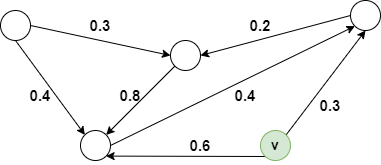
\includegraphics[width=\textwidth]{GSSI_thesisProposal/figures/ic1.png}
    \caption{At $t=0$}
    \label{fig:ic1}
\end{subfigure}
\hfill
\begin{subfigure}{0.3\textwidth}
    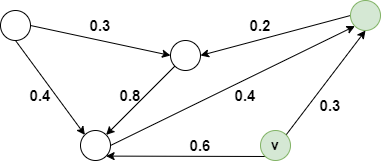
\includegraphics[width=\textwidth]{GSSI_thesisProposal/figures/ic2.png}
    \caption{At $t=1$}
    \label{fig:ic2}
\end{subfigure}
\hfill
\begin{subfigure}{0.3\textwidth}
    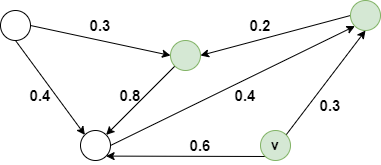
\includegraphics[width=\textwidth]{GSSI_thesisProposal/figures/ic3.png}
    \caption{At $t=2$}
    \label{fig:ic3}
\end{subfigure}
\caption{Diffusion process under the independent cascade at several time steps.}
\label{fig:cascade}
\end{figure}

\begin{figure}[!h]
\centering
\begin{subfigure}{0.3\textwidth}
    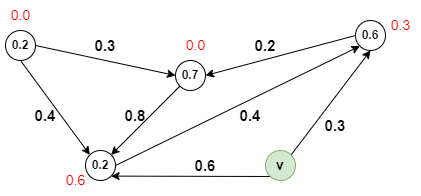
\includegraphics[width=\textwidth]{GSSI_thesisProposal/figures/lt1.png}
    \caption{At $t=0$}
    \label{fig:lt1}
\end{subfigure}
\hfill
\begin{subfigure}{0.3\textwidth}
    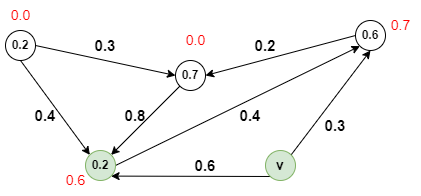
\includegraphics[width=\textwidth]{GSSI_thesisProposal/figures/lt2.png}
    \caption{At $t=1$}
    \label{fig:lt2}
\end{subfigure}
\hfill
\begin{subfigure}{0.3\textwidth}
    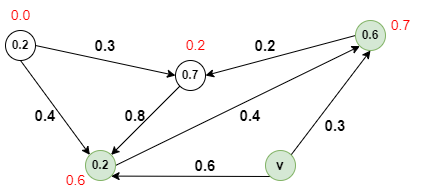
\includegraphics[width=\textwidth]{GSSI_thesisProposal/figures/lt3.png}
    \caption{At $t=2$}
    \label{fig:lt3}
\end{subfigure}
\caption{Diffusion process under the linear threshold at several time steps.}
\label{fig:linear}
\end{figure}





\subsection{Independent Cascade Model}

In the IC model, we have an {\em influence graph}  $G=(V=[n],E,(p_{uv})_{(u,v)\in E})$, where edges are directed and $p_{uv}\in [0,1]$ is an {\em activation probability} associated to each edge $(u,v)\in E$. Given a set of {\em seeds} $S\subseteq V$ which are initially \emph{active}, the diffusion process in the IC model is defined in $t\geq 0$  discrete steps as follows: (i) let $A_t$ be the set of active nodes which are activated at each step $t\geq 0$; (ii) $A_0:=S$; (iii) given a step $t\geq 0$, for any edge $(u,v)$ such that $u\in A_t$, node $u$ can activate node $v$ with probability $p_{uv}$ independently from any other node, and in case of success, $v$ is included in $A_{t+1}$; (iv) the diffusion process ends at a step $r\geq 0$ such that $A_{r}=\emptyset$, i.e., no more nodes in the graph can be activated. The size of $\bigcup_{t\leq r} {A_t}$, i.e. the number of nodes activated/reached by the diffusion process, is the {\em influence spread}. Figure \ref{fig:cascade} shows the influence unravelling at different time steps for the IC model.

We point out that the activation of an edge $(u,v)$ is a random event determined by the outcome of a coin toss that gives \textbf{head} with probability $p_{uv}$. Before the start of the diffusion process, the biased coin is flipped for every edge in the graph $G$. By looking at the influence probabilities; one can conclude whether a node $v$ will be active after the termination of the cascade process or not.

The above diffusion process can be equivalently defined as follows. The {\em live-edge graph} $\bm L=(V,\bm L(E))$ is a random graph of $G$, such that each edge $(u,v)\in E$ is included in $\bm L(E)$ with probability $p_{uv}$, independently from the other edges, i.e., $\mathbb{P}[\bm L=L]=\prod_{(u,v)\in L}p_{uv}\prod_{(u,v)\in E\setminus L}(1-p_{uv})$. 

With a little abuse of notation, we may denote $L(E)$ with $L$. Given $L\subseteq E$, let $R_L(S):=\{v\in V:\text{there exists a path from $u$ to $v$ in $L$ for some $u\in S$}\}$, i.e., the set of nodes reached by $S$ in the graph $L$. Informally, if $S$ is the set of seeds, and $L$ is a realisation of the live-edge graph, $R_L(S)$ equivalently denotes the set of nodes which are reached/activated by the above diffusion process. Let $\sigma_L(S):=|R_L(S)|$ denote the {\em influence spread} generated by the set of seeds $S$ if the realised live-edge graph is $L$, and let $\sigma(S):=\mathbb{E}_{ L}[\sigma_{{L}}(S)]$ be the {\em expected influence spread} generated by $S$. For a clear visualization of the realisations of a live-edge graph, refer to figure \ref{fig:real}.

Kempe et al.~\cite{Kempe2003} shows that finding the set of influential nodes maximizing the influence function in the IC model is NP-hard, and they use a reduction to the {\em Maximum Coverage} problem. A particular model of IC is that of \emph{Weighted Cascade}. In such a model, each influence probability is defined as $p_{uv}=1/d_{in}(v)$, where $d_{in}(v)$ is the in-degree of $v$. In this process, a node is equally influenced by each of its neighbours. 

Other models assume that the influence probabilities are not known. Saito et al.~\cite{Saito2008} predict the influence probabilities by using the \emph{Expectation Maximization} algorithm to compute the diffusion probabilities of all the edges in $G$,  repeatedly, to maximize the objective function. Goyal et al.~\cite{Goyal2010} developed a learning algorithm which takes as input a social graph and the \emph{Action Log}, that reports the actions performed by all the nodes. 


\begin{figure}[!h]
\centering
\begin{subfigure}{0.3\textwidth}
    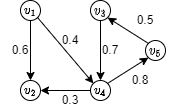
\includegraphics[width=\textwidth]{GSSI_thesisProposal/figures/real_1.png}
    \caption{Graph G}
    \label{fig:real_1}
\end{subfigure}
\hfill
\begin{subfigure}{0.3\textwidth}
    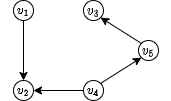
\includegraphics[width=\textwidth]{GSSI_thesisProposal/figures/real-2.png}
    \caption{Realisation $\phi_1$}
    \label{fig:real_2}
\end{subfigure}
\hfill
\begin{subfigure}{0.3\textwidth}
    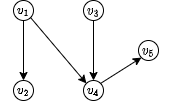
\includegraphics[width=\textwidth]{GSSI_thesisProposal/figures/real-3.png}
    \caption{Realisation $\phi_2$}
    \label{fig:real_3}
\end{subfigure}
\caption{A graph $G$ and two of its possible realisations.}
\label{fig:real}
\end{figure}


\subsection{Linear Threshold (LT) Model} \label{sec:lt}

Granovetter~\cite{Granovetter1978} introduced the \emph{Linear Threshold model}, where he proposed a diffusion model in which each node $v$ becomes active if the weighted sum of its active neighbours reaches a certain threshold. More formally, the model takes as input a graph $G$, the seed set $S$, and an edge weight $W_{u,v}$ for any edge $(u,v)\in E$. Before the diffusion starts, a \emph{threshold value} $\theta_v$ is picked uniformly at random in the interval $[0,1]$ by each node $v\in V$, independently from the other nodes.

At each time step $t$ a node $v$ will get activated if the summation of edge weights of its active neighbours reach the threshold value $\theta_v$, i.e.,  
\begin{equation}
\sum_{(u,v)\in E: u\text{ is active}} W_{u,v}  \geq \theta_u
\end{equation}
The process proceeds in several time steps and terminates when no more activations are possible. Figure \ref{fig:linear}, shows the steps of information diffusion in this model. The number inside the node indicates its threshold. A red counter on the side indicates the current active edge weight of a node. If the number in the red counter equals or exceeds the threshold of a specific node, then the node gets activated. Kempe et al.~\cite{Kempe2015} showed that finding the set $S$ maximizing the influence function in the LT model is also NP-hard, and they use a reduction to the {\em Vertex Cover} problem.  

A \emph{Generalized Threshold Model} can be designed by removing the linearity from LT. The model follows the same structure as LT. However, $v$ now relies upon an arbitrary {\em monotone threshold function} $f_v$ which maps the subsets of $v$’s neighbours into the interval $[0,1]$, with $f_v(\emptyset) = 0$. Let $N$ represent the set of neighbours of $v$ that are active at time step $t-1$. Node $v$ becomes active at time step $t$ if and only if $f_v(N) \geq \theta_v$. The LT model is a special case of the generalized threshold model. The threshold function of the LT model takes the following form:
\begin{equation}
f_v(N) = \min\left(1, \sum_{u \in N} W_{u,v}\right).
\end{equation}
The General Threshold model is {\em submodular} if each function $f_v$ is submodular. If this model is not submodular, its analysis may be intractable. 

\subsection{Triggering Model}

The IC and the LT are specialized cases of the \emph{triggering} model also introduced by Kempe et al.~\cite{Kempe2015}. In this model, instead of having a threshold value, a node $v$ has a quiescent subset $T_v$, called the \emph{triggering set}, which affects the state of $v$. Initially, the process starts with a seed set $S$, and each node $v$ chooses a triggering set $T_v$ independently from each other, according to some distribution over the subsets of its neighbours. An inactive node $v$ can be activated at time step $t$, if it has an active neighbour $u$ in $T_v$ at time step $t-1$.

Another way to think of this process is by considering the \emph{live-edge} technique. Edges of a graph $G=(V, E)$ can be either {live} or {blocked}. If a node $u$ is present in the triggering set $T_v$ of $v$, the edge $(u,v) \in E$ will be declared as live and claimed to be blocked otherwise. So, $v$ is reachable from the seed set $S$ by traversing a path made entirely out of live edges. The influence function $\sigma$ is shown to be submodular in the triggering model. 





\section{Non-Adaptive Influence Maximization}\label{nonada_sec}



The {\em non-adaptive influence maximization} is a computational problem, where given an influence graph $G$ and an integer $k\geq 1$, we are asked to find a set of seeds $S\subseteq V$ with $|S|\leq k$ such that $\sigma(S)$ is maximized. Without loss of generality, we assume that $k\in [n]$, and since the objective function is monotone, $|S|=k$ for any solution of $S$.

Kempe et al.~\cite{Kempe2003,Kempe2015} showed that function $\sigma$ is monotone and submodular, therefore the following greedy algorithm achieves a $1-\frac{1}{e}$ approximation factor. Algorithm \ref{algo:non} is as follows: (i) start with an empty set of seeds $S:=\emptyset$; (ii) at each iteration $t\in [k]$, add to $S$ the node $v$ that maximizes the expected influence spread $\sigma(S\cup \{v\})$. Note that the greedy algorithm requires at each iteration to compute the value of function $\sigma$, for some set of seeds.


\begin{algorithm}[ht]
	\caption{Non-Adaptive algorithm}
	\label{algo:non}
	\begin{algorithmic}[1]
		\REQUIRE an influence graph $G$;
		\STATE $S$ $\leftarrow$ $\emptyset$;
		\WHILE{{$|S| < k$}}
		\STATE $v^* \leftarrow \argmax_{v \in V \setminus S} (\sigma(S \cup \{v\})-\sigma(S))$;
		\STATE $S \leftarrow S \cup \{v^*\} $;
		\ENDWHILE
		\RETURN $S$;
	\end{algorithmic}
\end{algorithm}





\medskip

By using the fact that $\sigma$ is a monotone submodular function with $\sigma(\emptyset)=0$, the results of Nemhauser and Wolsey~\cite{Company1978} on submodular function approximation imply that algorithm \ref{algo:non} will always produce a solution guaranteeing at least $1-[(k-1)/k]^k\geq 1-1/e$ times the optimal value, where $e\simeq 2.71$ is the {\em Nepero number}.

At each step of algorithm \ref{algo:non}, we are required to compute the value $\sigma(S\cup\{v\})$ for any node $v\in V\setminus \{v\}$ to find the local optimal influence function, but this has been shown to be computationally intractable as it is $\#P$-hard~\cite{Chen10}. However, standard Chernoff bounds allow us estimate the value of $\sigma$ through a polynomial number of Monte-Carlo simulations by introducing an arbitrarily small additive error $\epsilon>0$, which depends on the number of simulations~\cite{Kempe2015}. In the reminder of the thesis, we will omit the additional term $\epsilon$ to avoid unnecessary complicated formulas (except for the experimental part, where we set $\epsilon=0.05$). We will refer to this algorithm as the \emph{non-adaptive greedy algorithm} in this thesis.

The two most widely studied non-adaptive IM algorithms are classified under the following categories: i) Monte-Carlo simulations-based approach \cite{Kempe2003} and, ii) Heuristic-based approach \cite{Borgs2014}.


\paragraph{Monte-Carlo simulation-based approach.} Kempe et al.'s non-adaptive greedy algorithm is an effective and simple algorithm that produces near optimal solution with a theoretical guarantee due to submodularity. They use Monte Carlo simulations to overcome the drawback of $\#P$-hard complexity. A Monte Carlo simulation is used to predict a model, by assigning a set of generated values based on a probability distribution to the uncertain variables. The simulations are computed independently on all the randomly generated values to obtain the results, which are then averaged to arrive at an estimate. Multiple instances of the graph $G$ are created and the number of reachable nodes $R(S)$ are computed for each of the generated instances. The value of $R(S)$ is averaged and the expected number of reachable nodes by S is $\sigma(S)$.

Nevertheless, the overhead cost that is incurred with a simple greedy algorithm is huge, because for each candidate seed node, the greedy algorithm simulates the influence cascade for estimating the influence increment. The number of Monte Carlo simulations required by the greedy algorithm is $O(mR)$, $O(m)$ is the time required for each simulation and $R$ is the number of simulations required ($R \approx 10000$ \cite{Kempe2003} for a good estimate). The resulting time complexity for the greedy algorithm is $O(kmnR)$, where $k$ is the total number of iterations, and $O(n)$ is the number of simulations for each iteration. 

Leskovec et al.~\cite{Leskovec2007} introduced the CELF algorithm which uses ``lazy-forward" optimization to improve on the time complexity for over 700 times by avoiding unnecessary simulations. They studied the structural property of social networks to find that real networks are mostly power-law graphs, which means majority of the nodes have a small influence. The algorithm maintains a priority queue to store the marginal influence of a node $v$ and the iteration number where it was computed. A node with a small influence in its previous iterations will not have a bigger marginal gain due to submodularity. Hence the simulation omit these nodes from its calculation without affecting the effectiveness of the algorithm.

The CELF algorithm was further improved by Goyal et al.~\cite{Goyal11} with CELF++ which ran $35\%-55\%$ faster than CELF. Other simulation based approaches include that of Cheng et al.~\cite{DBLP:conf/cikm/ChengSHZC13} to reduce the number of computations of CELF. Another simulation based paper was by Ohsaka et al.~\cite{DBLP:conf/aaai/OhsakaAYK14}, where they prune the number of BFSs required for reachability tests by reducing the number of vertices visited during each BFS. However, Monte Carlo simulations are computationally expensive and has scalibility issues when the graph starts to grow. 

\paragraph{Heuristic-based approach.}

In order to tackle with the expensive computations and large-scale networks,
Chen et al.~\cite{DBLP:conf/kdd/ChenWY09} used the degree discount technique which reduces the running time but has a much lower efficiency compared to the Monte Carlo approach. Borgs et al.~\cite{Borgs2014} introduced the \textit{reverse sampling technique (RIS)} and utilizes the concept of \textit{reverse reachable (RR) sets} and \textit{Random RR sets}. An instance $g$ of graph $G$ is generated by using the value of $p_{(uv)}$ to add edges in $g$ between nodes $u$ and $v$ of $g$. The RR set for a node $u$ in $g$ is the set of nodes that have a directed path to $u$ in $g$. Due to the randomness of generating $g$ using the probability on edges, we have a distribution $\mathcal{G}$ of $g$. To generate a random RR set on $g$, the instance $g$ is randomly sampled from $\mathcal{G}$. 

The idea behind Borgs et al.'s algorithm RIS, is to generate a large set of random RR sets, denoted as $\mathcal{R}$. Using the greedy maximum coverage algorithm from \cite{Vazirani} the goal is to find a seed set $S^*$ of size $k$ which covers the maximum number of RR-sets, this implies that $S^*$ will have the maximum expected spread over all the size $k$ seed sets of $G$. Borgs et al.'s technique reduces the estimation of a large number of node sets hence reducing the overhead time complexity induced by simulation based approaches. To calculate the number of RR sets that needs to be generated, RIS proposed a predefined threshold value $\tau$. Defining a proper $\tau$ value results in a seed set $S$ being generated at almost linear time complexity with an approximation ratio of $(1-\frac{1}{e}-\epsilon)$. The RIS still has some overhead cost due to the dependency of $\tau$ on the number of nodes and edges examined.

Tang et al.~\cite{Tang2014} provided an improved version of the RIS algorithm called $TIM^+$. They mainly cut down the threshold cost by replacing it with a predefined constant $\theta$. TIM removes the dependency from the edges, and uses Chernoff bounds to estimate the value for $\theta$. The estimated time complexity of the $TIM^+$ algorithm is $O((k+l)(m+n)\text{log} n/\epsilon^2)$, where $l$ is a constant and is set to $1$. For the experimental part of the thesis (section \ref{exp}), we use $TIM^+$ as the base non-adaptive greedy algorithm.
Tang et al.~\cite{Tang15} further improved on the efficiency of $TIM^+$ with the IMM algorithm by bounding the size of $\mathcal{R}$ using a martingle approach.

More improvements on the IMM algorithm was brought by Nguyen et al.~\cite{Nguyen16}, Huang et al.~\cite{Huang}, Tang et al.~\cite{Tang2019} where they curb the excessive generation of RR sets when the value of $k$ is large. They work with the \textit{Stop-and-Stare} algorithm \cite{Nguyen16}, where they set a stopping time limit $T$. The sampling process is stopped when $T$ is reached and the algorithm checks if the seed set $S$ fulfils the $(1-1/e-\epsilon)$-approximation. Once the current $S$ reaches the approximation, the algorithm terminates. 


The heuristic-based approach has better scalibility and time complexity, but lacks in the department of performance guarantees that the simulation-based approach can provide.

 


\section{Adaptive Influence Maximization} \label{sec:aim}


\subsection{Adaptive Maximization} 


Golovin and Krause~\cite{Golovin2011} studied the {\em Adaptive Maximization (AM)} setting, and later applied it to the context of Influence Maximization by introducing its adaptive version. The general problem of AM is defined as follows: consider a graph $G=(V,E)$ and a set of states $O = \{alive, dead\}$. Each edge $e \in E$ is in one of the possible states, so that the state of the edges can be represented using a function $\phi: E \mapsto O$, called the \emph{realisation}. Hence, we can state that $\phi(e)$ is the state of $e$ under realisation $\phi$. A random variable $\Phi$ taking values from all the possible realisations, according to a given probability distribution, is called a {\em random realisation}. For a given realisation $\phi$, let $p(\phi)$ denote the probability that $\Phi=\phi$.

We probe each $e \in E$ sequentially and observe its state $\Phi(e)$. The observations made after each pick can be represented as a \emph{partial realisation} function $\psi$, over some subset of $E$. The domain of $\psi$, i.e., the set of edges observed in $\psi$ is represented by $dom(\psi)$. A partial realisation function is said to be consistent with a realisation $\phi$ if they are equal in $dom(\psi)$ and is written as $\phi \sim \psi$. When $\psi$ and $\psi’$ are both consistent with some $\phi$, and $dom(\psi) \subseteq dom(\psi’)$, $\psi$ is called the \emph{subrealisation} of $\psi’$. 

The node selection for the next round is strategized by an \emph{adaptive policy} $\pi$, which is a function from a set of partial realisations to $E$. When $\psi$ is not present in the domain of $\pi$, the termination of the policy occurs upon observations of $\psi$. The domain of $\pi$, denoted by $dom(\pi)$, should be closed under subrealisations. The function we want to maximize is in the form of $f:2^E\times O^E\rightarrow \mathbb{R}_{\geq 0}$, and takes as input the realisation $\phi$, and the set of edges $E(\pi, \phi)$ selected by the considered adaptive policy $\pi$ under realisation $\phi$. Unfortunately, we do not know what is the final realisation $\phi$. The AIM overcomes this problem, and its goal is to find a policy $\pi^*$ that maximizes the expected value $\mathbb{E}_{\Phi}(f(E(\pi,\Phi),\Phi))$ subject to $E(\pi,\Phi)\leq k$, where $k$ is the maximum number of edges that a policy can select.





\subsection{Adaptive Influence Maximization} 
Now, we adapt the previous framework of adaptive maximization to the IM problem and get the AIM Problem.
Differently from the non-adaptive setting, in which all the seeds are selected at the beginning, an adaptive policy activates the seeds sequentially in $k$ steps,
one seed at each step, and the decision on the next seed to select is based on the feedback resulting from the observed spread of previously selected nodes. The feedback models considered in this work are the full-adoption feedback: where the adaptive policy observes the entire spread of the selected seed node; and myopic: when a node is selected, the adaptive policy observes just the state of its neighbours. 
Chapters \ref{chap:background} and \ref{chap:sota} provide the technical definitions related to the adaptive influence maximization under specific feedback models.


\paragraph*{Adaptivity Gap.} The adaptivity gap on an input instance is defined as the ratio between the optimal adaptive policy and the optimal non-adaptive policy. Since an adaptive policy is strictly better than a non-adaptive one, if the value of AG is closer to 1, the non-adaptive policy is considered to be as efficient as the adaptive policy, and we can use the non-adaptive policy as a good approximation to the adaptive one, due to its simplicity. Chapter \ref{chap:background} Section \ref{ag} provides a more formal definition of the adaptivity gap.






\subsection{Feedback Models of AIM} \label{feedback}
Depending on the type of network state that a policy can observe at each time, we have two general models of AIM: {\em edge-feedback model}, in which the network state is a set of active edges, and {\em node-feedback model}, in which the network state is a set of active nodes.

In this section, we discuss some particular models of AIM, that can be either node-feedback, or edge-feedback. In particular, here we discuss the full-adoption feedback, myopic feedback, and the \emph{general feedback} model under the edge feedback.

\subsubsection{Full-Adoption Feedback Model} \label{full_adop}

The full-adoption feedback selects a node and returns the entire cascade as feedback for the next round. Each node is selected one by one, and the selection needs to be done at the beginning of each round. Once the budget $k$ is reached, the process terminates and returns the seed set. To solve the AIM problem in the full-adoption feedback model, Golovin and Krause~\cite{Golovin2011} designed an adaptive version of the non-adaptive greedy algorithm.
Golovin and Krause \cite{Golovin2011} showed that the full adoption feedback can guarantee a good approximation ratio by applying the concepts of monotone and submodular functions to the adaptive framework.

The algorithm greedily selects nodes one by one from the graph $G$ until the budget $k$ has been reached. For each node $u \in V$, the conditional expected marginal gain is determined. The node with the largest estimate for the gain is added to $S$, and the random realisation of the selected node $u$ is observed. The set of partial realisations is updated by adding the edges that has been activated by $u$. Golovin and Krause~\cite{Golovin2011} proved that for the adaptive IM problem, the greedy policy $\pi^G$ determined by a greedy adaptive algorithm achieves at least $\left(1- \frac{1}{e}\right)$ of the optimal policy, when $f$ is adaptive monotone and submodular. 

Nevertheless, the greedy adaptive algorithm can not reach the above approximation guarantee in polynomial time, because to select a seed node adaptively in each round, we need to identify the node $u$ with the highest expected spread on the residual graph $G_u$, which is obtained by removing all the activated nodes from the previous rounds via the feedback. However, computing the exact spread is $\#P$-hard \cite{Chen10}. Vaswani and Lakshmanan~\cite{Vaswani2016} overcame this drawback by allowing errors on the expected spread estimation. By introducing a parameter $\eta$ to bound the error and using the greedy approach of Dar and Shapira~\cite{Even-Dar2007}, an approximation guarantee of $1-1/e^\eta$ is reached. Vaswani and Lakshmanan also extended their approach to batch mode, where instead of selecting one seed node and observing the influence, we can select a batch of seed nodes, and observe its spread to do the node selection for the next batch.


Together with the problem of finding an optimal adaptive policy, determining the adaptivity gap for the full adoption feedback is also a challenge. Chen and Peng~\cite{Chen2019} derive the upper and lower bounds on the AG when the graphs are \emph{in-arborescences} and \emph{out-arborescences}. An arborescence is a directed rooted tree. An in-arborescence (resp. out-arborescense) is an arborescence when the edges are directed from the leaves to the root (resp. from the root to the leaves).

Since the information propagates from the leaves to the root in an in-arborescence, the boundary of active nodes shrinks. The leaves are the set of discovered nodes, and the boundary forms the subset of the set of nodes reachable from the leaves. Using these properties, the AG has been shown to be between $\frac {e}{(e-1)}$ and $\frac{2e}{(e-1)}$. In the case of an out-arborescence graph, the main observation has been that the predecessors of each node in the graph forms a directed line. In order to activate a certain node $u$, all its predecessors must be activated one at a time. For out-arborescences the AG has been shown to be between $\frac {e}{(e-1)}$ and $2$.


\subsubsection{Myopic Feedback Model}

The main drawback of the full adoption feedback model is the delay in the process: select nodes one by one, observe its complete diffusion, return it as a feedback for the selection of the next seed node, and continue this over $k$ steps. To overcome this potential set back, we could select a seed node $u$ and check which of its neighbours are getting influenced by it, and return the set of neighbours influenced by $u$ as a feedback for the next round. Since only the active neighbours of the selected seeds are returned as feedback, the model is called myopic. The myopic model has been mentioned by Golovin and Krause~\cite{Golovin2011}, and in a revised arXiv version of the same paper, the authors claimed that the objective function $f$ in the myopic feedback model is not adaptive submodular. The adaptive submodularity condition is violated since the seed node selection process is not made after a diffusion terminates. Instead, the diffusion of a certain round ceases after the current node activates its neighbours. 

Peng and Chen~\cite{Peng2019} confirmed the conjecture of Golovin and Krause~\cite{Golovin2011}, which states that the adaptive greedy algorithm with myopic feedback is a constant approximation of the adaptive optimal solution. They obtain an upper and lower bound for the AG under the IC model with myopic feedback, $[\frac {e}{e-1}, 4]$.  They also proved that the adaptive and the non-adaptive greedy algorithms have an approximation ratio of $\frac{1}{4}(1-\frac{1}{e})$ under the myopic model. The authors conclude by stating that the myopic feedback is not beneficial since the approximation ratios for both the adaptive and non-adaptive greedy algorithms are the same. Also, the solution is $\frac{e^2+1}{(e+1)^2} \approx 60\%$ of the optimal value, which is less than the results obtained by Kempe et al.~\cite{Kempe2015}. In simple words, the performance is not commendable since the feedback received is not enough to determine the selection of the best possible node in the next round. However, for both practical and theoretical reasons, studying the myopic model is useful.


\subsubsection{Partial and General Feedback Model}

Yuan and Tang~\cite{Yuan2017} have expressed the trade-off between performance and delay in the full adoption and the myopic feedback model. They developed the \emph{partial feedback} model, which however is not adaptive submodular, due to the same reasons as the myopic model. The partial feedback model can capture a more realistic scenario of the marketing world. The model considers a general {\em $\alpha$-greedy policy}, depending on a {\em control parameter} $\alpha\in [0,1]$ given as input. At each round $r$, a policy selects a new seed node $v$, and the cascade proceeds via {\em time slots} in which the depth of the cascade increases by one; we can equivalently denote each time slot with the depth $d$ of the cascade generated by $v$. At each round $r$ and time slot $d$, the policy observes the state of all the edges involved in the cascade, and the round ends when the following condition is verified:
\begin{equation}
\alpha \leq \frac{\sum_{v \in V} p_v(S_r, \psi_{r,d})}{|V \setminus O_{r,d}|}, 
\end{equation}
where $\psi_{r,d}$ represent the observations, $O_{r,d}$ represents the set of nodes whose activation probabilities are zero at round $r$ and at time slot $d\geq 0$, and $\sum_{v \in V} p_v(S_0, \psi_{r,d})$ is the expected number of activated nodes, under the activation probability of $p_v(S_r, \psi_r)$, with $S_r$ being the seed set. After this, a new round starts, and the previous process continues iteratively until the seed set contains $k$ nodes. Informally, each round terminates when the expected probability that a node becomes active is higher than $\alpha$. Observe that, the partial model becomes a full adoption feedback when $\alpha = 1$, and non-adaptive IM when $\alpha = 0$. 

Tong and Wang~\cite{Tong2019} introduced the \emph{general feedback} model. Such a model is defined as the partial model, except for the fact that each round terminates after exactly $d$ time slots, where $d\geq 0$ is an integer given as input. Observe that for $d=1$ we get the myopic feedback, and for $d=\infty$ we get the full adoption feedback model.  Since the model is not adaptive submodular, one cannot immediately guarantee that the greedy strategy is a good approximation algorithm. To overcome this problem, the authors introduced a new metric called the \emph{regret ratio}. The regret ratio $R$ of a diffusion process is the maximum ratio between (i) the best marginal profit obtained for a given seed set and a given round, when a new seed node is added to $S$ at the beginning of round $r$, and (ii) the best marginal profit achieved when the new seed node is added to $S$ at the end of round $r$, i.e., after $d$ time slots. The regret ratio has been used to show that the greedy algorithm guarantees an approximation factor of $1-e^{-1/R}$. 
 

\subsection{Multi-Round Influence Maximization}
Sun et al.~\cite{Sun2018} works on a marketing scenario, where the advertiser considers multiple rounds to market a product. In particular, instead of considering one round for the diffusion process, the advertiser conducts the diffusion process over $T$ rounds. The advertiser has a budget $k$ for each round, i.e., a seed set $S_t$ of at most $k$ nodes can be selected at each round. An independent diffusion process is carried out in each round $t$, where a subset of nodes are activated, starting from the initial seed set $S_t$. The total influence spread over the $T$ rounds is calculated as the union of the sets of nodes activated over all the $T$ rounds. The goal is to find the seed sets that maximize the expected total influence spread. The authors work on both the adaptive and non-adaptive version and design three greedy algorithms.

In the non-adaptive version, the advertiser needs to find all the $T$ seed sets before the start of the diffusion process. The authors consider two different algorithms: \emph{cross-round} and \emph{within-round}.
The within-round has an approximation ratio of $1-e^{-(1-\frac{1}{e})} \approx 0.46$. However, the cross-round has a better approximation factor of $1/2 - \varepsilon$, but has a higher running time. 

For the adaptive version, in each round, the advertiser needs to select the seed set for that round and observe its influence spread. Once the budget $k$ is reached for a specific round $r$, the next round $r+1$ receives the influence spread of the previous $r$ rounds as feedback. In the next round, based on the observations of the propagation made by the previous rounds, the seed set for that round is selected. The authors designed a greedy approximation algorithm called \emph{AdaGreedy}, and show that the algorithm guarantees a $1-e^{-(1-\frac{1}{e})} - \varepsilon$ approximation ratio.


\subsection{Other variations of AIM} \label{sec:var}


\paragraph{Non-monotone models.}
 Gotovos et al.~\cite{gotovos} proposed the \textit{adaptive random greedy policy} which generalizes the random greedy algorithm by Buchbinder et al.~\cite{buchbinder}. The policy can be used for both monotone and non-monotone functions, however for non-monotone functions the policy achieves a $1/e$ approximation ratio. The algorithm introduces dummy nodes to the ground set which ensures that the algorithm never picks a node with a negative marginal gain. Instead of selecting the node with the highest marginal gain, the algorithm randomly selects a node from a set, which contains k-nodes with the highest marginal gain.



The time required for the algorithm is majorly dependent on the number of times the objective function is evaluated and it is $O(nk)$ for \cite{gotovos} which is their main drawback. Tang~\cite{TANG2021249} proposes a linear-time policy for the same problem, where the time is not dependent on the value of $k$ and requires $O(\frac{n}{\epsilon^2}\frac{1}{log \epsilon})$ evaluations achieving the same approximation factor of $1/e$. Their algorithm also speeds up on the monotone variant of the problem. The idea behind their policy is to sample a random set of size $min[qn,n]$, where $q$ is a parameter dependent on the value of $k$ and used to bound the time. Out of that random set, the seed with the $i$-th largest marginal gain w.r.t the current partial realisation is selected, where $i$'s value is sampled at random from $(0,s]$, and $s$ is another parameter relying on $n$ and $k$. If the selected node's marginal gain is non-negative, it is added to the seed set. 

A recent work of Amanatidis et al.~\cite{amanatidis} on non-monotone adaptive submodular function subject to knapsack constraints, which are more stringent by nature, achieves a constant factor approximation and runs $O(n log(n))$ evaluations.

\paragraph{DR-submodularity.} Guo and Wu~\cite{guo} studied AIM when the model is adaptive DR-submodular or \textit{diminishing return submodular}. DR-submodularity is a generalization of the submodularity property and are generally defined over integer lattices (seeding vectors) instead of seed sets. Inspired by the works of Chen et al.~\cite{drchen} on influence maximization over lattices, Guo and Wu extended their work to the adaptive setting. They consider a new scenario where after activating a seed node, we wait to see if the selected node is willing to be the seed node. If the selected node refuses to be the seed, we either raise the cost of the selected seed to be the seed, or we select a new node to become the seed. Only when a node accepts to be the seed, we move on to observing its spread. They named this the \textit{Adaptive-IMMA} problem which stands for AIM with multiple activations. They show that the AIM problem with dr-submodularity returns an approximation ratio of $(1-1/e)$.



\section{Stochastic Multi-Value Probing (SMP)}\label{smp}

Previous works on finding the adaptivity gap under independent cascade includes the usage of the stochastic multi-value probing model which was introduced in the adaptive setting by Bradac et al.~\cite{Bradac19}. The SMP problem is a generalized version of the stochastic probing model, whose adaptive version was studied by Gupta et al.~\cite{Gupta2017}.

The stochastic probing model is defined as follows, we are given an universal set $V = [n]$ and set of edges $E$ with all the combination of possible edges. Each of these edges $e \in E$ has a probability $p_e$ associated with it and denotes the activation probability of $e$. We have a set $A \subseteq V$ chosen at random from a family of subsets of $V$, $\mathcal{S}$. We probe each of the elements, $v \in A$ to reveal whether $v$ is active in $A$ or not due to the probability on the edges. However, we are only allowed to probe certain subsets $S \in \mathcal{S}$, which fulfills the budget requirements (constraints). The goal here is to find a probing strategy that maximizes the expected number of active nodes in the set $A$, which is $\mathbb{E}_A[f(A \cup S)]$.  


The utility function is monotone submodular and the probing strategy can be transformed to an adaptive setting, where after probing each element $v \in A$, we observe its outcome, and then continue with the next probe. The adaptive probing strategy is designed using a binary rooted decision tree, $\mathcal{T}$. The nodes in the tree represents the elements in the ground set $V$, and each of these nodes (except  the leaves) have two outgoing edges, $yes$, when the edge $e$ is active with probability $p_e$, and $no$, when the edge $e$ is inactive with probability $1-p_e$. Note that when the edge is active, it automatically activates the inactive node, its direct child. The probing process terminates, when we reach the leaf nodes, where no more activations are possible. The stem of a tree represents the path of unsuccessful probes. Whenever a stem is observed, it is stitched back to the root which causes a loss and the final adaptivity gap becomes 3 \cite{Gupta2017}. 

The above mentioned problem can be generalised by using more than the Bernoulli random variables, and allowing multiple values on the edges. Bradac et al.~\cite{Bradac19} considered adding multiple values to the edges of the rooted decision tree $\mathcal{T}$, which no longer restricts itself to binary values. Due to the loss caused by sticking back of the stem to perform the induction over its subtrees, Bradac et al.~\cite{Bradac19} observes at each step a single node, instead of an entire stem and thus retrieving the loss and upper bounding the AG to 2. 

The idea is the following, we have a non-adaptive strategy that randomly chooses a path in the decision tree with the same probability as an optimal adaptive strategy would have. This randomised non-adaptive strategy can be described as follows:
starting from the root, one of its children is probed randomly with the same probability that the optimal adaptive policy would have probed this child. The result is stored under a partial realisation $T_{v1}$, and the iteration continues till a leaf is reached. The non-adaptive policy selects this path from the root to the leaf.


By combining the non-adaptive policy with optimal adaptive policy, Bradac et al.~\cite{Bradac19} defines the super adaptive strategy, which gives a node two chances of probing. For any $i \geq 1$, when the non-adaptive policy decides to include the $i$-th node in the path towards the leaf node, we notice that the expected increment in the utility of the non-adaptive policy will be at least half of the expected increment achieved by the super adaptive strategy.
Asadpour and Nazerzadeh~\cite{Asadpour16} showed that the adaptivity gap of SMP under cardinality constraints is upper bounded by 1.58.
Where as, Bradac et al.~\cite{Bradac19} proved that the upper bound of adaptivity gaps under the downward-closed families of set constraints (cardinality, knapsack and matroid), which means if a set can be probed, even their subsets can be probed, are 2 and tight for both the theorems \cite{Asadpour16,Bradac19}.


Using the above techniques to find the adaptivity gap for SMP problems, Chen and Peng~\cite{Chen2019} studied different graph classes with AIM under full adoption and IC. They use multilinear extension and Poisson process from \cite{Asadpour16} to model the AIM problem as a SMP problem. Since the results of \cite{Asadpour16} are based on cardinality constraints, modelling it for the IM problem becomes easier.
For myopic feedback under IC, Peng and Chen \cite{Peng2019} relies on the decision tree technique from \cite{Bradac19} to build the artificial diffusion model, which gives each seed multiple chances to influence its neighbour and bound the AG for the myopic model. 


The techniques involved in this thesis are inspired from the literature above, however, we resort to a simpler and direct analysis to get better bounds on the adaptivity gap under IC with both the feedback models.
%----------------------------------------------------------------------------------------
%	AAAI paper
%----------------------------------------------------------------------------------------


\chapter{Better bounds on the Adaptivity Gap of Influence Maximization under Full-Adoption feedback}\label{chap:background}
\fancyhead[L]{\textit{Chapter 3. Better Bounds on Adaptivity Gap}}


In this chapter, we consider the independent cascade model with full-adoption feedback, and show the first sub-linear upper bound on the adaptivity gap, (ratio between the optimal adaptive policy and the optimal non-adaptive policy [\ref{ag}]) that holds for general graphs. In detail, we show that the adaptivity gap is at most $\lceil n^{1/3}\rceil$ (Theorem~\ref{thrm2}), where $n$ is the number of nodes in the graph. Moreover, we tighten the upper bound on the adaptivity gap for in-arborescences by showing that it is at most $\frac{2e^2}{e^2-1}<\frac{2e}{e-1}$ (Theorem \ref{thrm1}).


Using similar techniques, we study the adaptivity gap of two classes of influence graphs: \emph{$\alpha$-bounded-degree graphs}, which is the class of influence graphs where the sum of node degrees higher than two is at most $\alpha$, and \emph{$(\beta,\gamma)$-bounded-activation graphs}, where the nodes are partitioned into influential nodes, which are at most $\beta$ nodes, and non-influential, where each of these nodes can infect at most $\gamma$ neighbours in expectation, where the value of $\gamma$ is less than 1. $\alpha$-bounded-degree graphs can be encountered in several graph topologies (see, for instance, Example \ref{exam1}), and $(\beta,\gamma)$-bounded-activation graphs are well-motivated by social networks in which most nodes have a limited power of influence. We show that the adaptivity gap of $\alpha$-bounded-degree and $(\beta,\gamma)$-bounded-activation graphs is upper-bounded by $\sqrt{\alpha}+O(1)$ and $\sqrt{\beta}+\frac{1}{1-\gamma}$ (Theorems \ref{thmlast} and \ref{thmlast2}) respectively, and these values are smaller than that of $O(n^{1/3})$ for several influence graph classes. Furthermore, in 0-bounded-degree graphs, i.e. undirected graphs in which each connected component is a path or a cycle, the adaptivity gap is at most $\frac{3e^3}{e^3-1}$ (Theorem~\ref{thm_0bou}). 
%

To prove our bounds, we introduce new techniques to connect adaptive policies with non-adaptive ones that might be of their own interest (further details are given in the paragraph ``General outline of the proof technique'' in Section \ref{sec_inarb}). In particular, we resort to a simple randomized {\em hybrid non-adaptive policy}, that differs from the main approaches previously used in adaptive influence maximization and other adaptive optimization problems:  (i) the {\em Poisson process} \cite{norris} combined with the {\em multi-linear extension of submodular set-functions} \cite{Calinescu11}, which represent the main probabilistic technique adopted by \citet{Asadpour16} and \citet{Chen2019}, and (ii) the {\em random walk on the decision tree} \cite{AdamczykGM15,sahil}, that is a tool applied by \citet{Gupta2017,Bradac19} and \citet{Peng2019}.

In the experimental section \ref{exp}, we take into account a cutting age non-adaptive greedy algorithm, called $TIM^+$, and design its adaptive version to compare their performance ratio, called the greedy adaptivity gap. To compute the efficiency of the seed set selected by $TIM^+$, we design another adaptive algorithm, which take as input the predetermined seed set selected by $TIM^+$, and running the adaptive algorithm on top of it. We observe that the ratio is closer to one, thus implying the efficiency of $TIM^+$ when compared to its adaptive counterpart.  

\subsection*{Related Works.}
Adaptivity gaps for the problem of maximizing stochastic monotone submodular functions have been studied by \citet{Asadpour16}. There exists a series of work engaged with adaptivity gaps for a two-step adaptive influence maximization problem~\cite{Badanidiyuru2016,Rubinstein2015, Seeman2013, Singer2016}. Gupta et al.~\cite{sahil, Gupta2017} and \citet{Bradac19} worked on the adaptivity gaps for stochastic probing. 

A recent line of studies~\cite{Chen2019, Chen2019a, Peng2019} focuses on finding the adaptivity gap on different graph classes using the classical feedback models. \citet{Peng2019} confirmed a conjecture of \citet{Golovin2011a}, which states that the adaptivity gap of the independent cascade model with myopic feedback is constant. In particular, they showed that the adaptivity gap belongs to $[\frac{e}{e-1}, 4]$. \citet{Chen2019a} introduced the greedy adaptivity gap, which compares the performance of the adaptive and the non-adaptive greedy algorithms. They show that the infimum of the greedy adaptivity gap is $1-\frac{1}{e}$ for every combination of diffusion and feedback models.

The most relevant related work to our results in this chapter is that of \citet{Chen2019}, as they derive upper and lower bounds on the adaptivity gap under the independent cascade model with full-adoption feedback, when the considered graphs are in-arborescences, out-arborescences, or one-directional bipartite graphs. In particular, they show that the adaptivity gaps of in-arborescences and out-arborescences are in the intervals $\left[ \frac{e}{e-1}, \frac{2e}{e-1}\right]$ and $\left[ \frac{e}{e-1}, 2\right]$ respectively, and they provide a tight bound of $\frac{e}{e-1}$ on the adaptivity gap of one-directional bipartite graphs. Under the more general triggering model, a constant upper bound of $2$ on the adaptivity gap of one-directional bipartite graphs was provided by \citet{Fujii2019}.


\subsection*{Contributions.}
Our main notable result in this chapter is the first sub-linear upper bound that holds for any graph. Specifically, we show that the adaptivity gap is upper-bounded by $\lceil n^{1/3}\rceil$, where $n$ is the number of nodes in the graph. Moreover, we improve over the known upper bound for in-arborescences from $2e/(e-1)\approx 3.16$ to $2e^2/(e^2-1)\approx 2.31$. 

Then, we study $\alpha$-bounded-degree graphs, that is the class of undirected graphs in which the sum of node degrees higher than two is at most $\alpha$, and show that the adaptivity gap is upper-bounded by $\sqrt{\alpha}+O(1)$; we also show that in 0-bounded-degree graphs, i.e. undirected graphs in which each connected component is a path or a cycle, the adaptivity gap is at most $3e^3/(e^3-1)\approx 3.16$. 

We also consider $(\beta,\gamma)$-bounded-activation graphs \cite{AIJ}, where all nodes but $\beta$ influence in expectation has at most $\gamma\in [0,1)$ neighbors each; for this class of influence graphs we show that the adaptivity gap is at most $\sqrt{\beta}+\frac{1}{1-\gamma}$. To prove our bounds, we introduce new techniques to relate adaptive policies with non-adaptive ones that might be of their own interest. 


Finally, we have some experiments to determine the performance efficiency of a specific widely used non-adaptive greedy algorithm, $TIM^+$. We build a greedy adaptive equivalent of $TIM^+$ and discuss about the quality of seed set generated by both the versions of $TIM^+$, the memory, and time overhead. We conclude that $TIM^+$ as a greedy non-adaptive algorithm performs quite well when compared to its adaptive counterpart and the main focus should be on the requirements of the computational costs to run these algorithms.

\subsection*{Organization of the Chapter.}
The preliminaries for this chapter is defined in Section~\ref{sec_prel}. Sections~\ref{sec_inarb}--\ref{sec_other} are devoted to the main technical contribution of the chapter, i.e., upper bounds on the adaptivity gap of in-arborescences, general graphs and other influence graphs ($\alpha$-bounded-degree and $(\beta,\gamma)$-bounded-activation graphs). Section \ref{exp} has some experiments comparing the results of $TIM^+$, adaptive greedy under $TIM^+$, and adaptive greedy with the seeds generated by $TIM^+$ for different network types and parameters under the IC and LT models. 

\section{Preliminaries}\label{sec_prel}
For two integers $h$ and $k$, $h\leq k$, let $[k]_h:=\{h,h+1,\ldots, k\}$ and $[k]:=[k]_1$. 

\paragraph*{Non-adaptive Influence Maximization} The {\em non-adaptive influence maximization problem under the IC model} is a computational problem that is defined as follows: given an influence graph $G$ and an integer $k\geq 1$, we are asked to find a set of seed nodes $S\subseteq V$ with $|S|=k$ such that $\sigma(S)$ is maximized. Without loss of generality, we assume that $k\in [n]$ and, since the objective function is monotone, $|S|=k$ for any solution $S$. A detailed overview is presented in Sections \ref{main}--\ref{nonada_sec} of Chapter \ref{chap:lit}. 

\paragraph*{Adaptive Influence Maximization} Differently from the non-adaptive setting, in which all the seed nodes are activated at the beginning and then the influence spread is observed, an {\em adaptive policy} activates the seeds sequentially in $k$ steps,
one seed node at each step, and the decision on the next seed node to select is based on the feedback resulting from the observed spread of the previously selected nodes. The feedback model considered in this work is {\em full-adoption}: when a node is selected, the adaptive policy observes its entire influence spread. 

An adaptive policy under the full-adoption feedback model is formally defined as follows. Given a live-edge graph $L$, the {\em realization} $\phi_L:V\rightarrow 2^V$ associated to $L$ assigns to each node $v\in V$ the value $\phi_L(v):=R(\{v\},L)$, i.e., the set of nodes activated by $v$ under a live-edge graph $L$. Given a set $S\subseteq V$, a {\em partial realization} $\psi:S\rightarrow 2^V$ is the restriction to $S$ for some realization, i.e., there exists a live-edge graph $L$ such that $\psi(v)=\phi_L(v)$ for any $v\in S$. Given a partial realization $\psi:S\rightarrow 2^V$, let $dom(\psi):=S$, i.e., $dom(\psi)$ is the domain of  partial realization $\psi$, let $R(\psi):=\bigcup_{v\in S}\psi(v)$, i.e., $R(\psi)$ is the set of nodes reached/activated by the diffusion process when the set of seed nodes is $S$, and let $f(\psi):=|R(\psi)|$. A partial realization $\psi'$ is a {\em sub-realization} of $\psi$ (or, equivalently,  $\psi'\subseteq \psi$), if $dom(\psi')\subseteq dom(\psi)$ and $\psi'(v)=\psi(v)$ for any $v\in dom(\psi')$. We observe that a partial realization $\psi$ can be equivalently represented as $\{(v,R(\{v\},L)):v\in dom(\psi)\}$ for some live-edge graph $L$. 

An adaptive policy $\pi$ takes as input a partial realization $\psi$ and, either returns a node $\pi(\psi)\in V$ and activates it as seed, or interrupts the activation of new seed nodes, e.g., by returning a string $\pi(\psi):=STOP$; furthermore, we assume (w.l.o.g.) that an adaptive policy $\pi$ chooses each seed based only on the observation of $R(\psi)$ (i.e., the set of nodes activated by the previous seeds) and $|dom(\psi)|$ (i.e., the number of seeds previously selected), that is, $\pi(\psi)=\pi(R(\psi),|dom(\psi)|)$. An adaptive policy $\pi$ can be run as in Algorithm \ref{ad_alg}. The {\em expected influence spread} of an adaptive policy $\pi$ is defined as $\sigma(\pi):=\mathbb{E}_L[f(\psi_{\pi,L})]$, i.e., it is the expected value (taken on all the possible live-edge graphs) of the number of nodes reached by the diffusion process at the end of Algorithm \ref{ad_alg}. We say that $|\pi|=k$ if policy $\pi$ always return a partial realization $\psi_{\pi,L}$ with $|dom(\psi_{\pi,L})|=k$. The {\em adaptive influence maximization problem under the IC model} is the computational problem that, given an influence graph $G$ and an integer $k\geq 1$, asks to find an adaptive policy $\pi$ that maximizes the expected influence spread $\sigma(\pi)$ subject to a constraint $|\pi|=k$. 
\begin{algorithm}[ht]
	\caption{Adaptive algorithm}
	\label{ad_alg}
	\begin{algorithmic}[1]
		\REQUIRE an influence graph $G$ and an adaptive policy $\pi$;
		\ENSURE a partial realization;
		\STATE let $L$ be the live-edge graph;
		\STATE let $\psi:=\emptyset$ (i.e., $\psi$ is the empty partial realization);
		\WHILE{$\pi(\psi)\neq STOP$}
		\STATE $v:=\pi(\psi)$;
		\STATE $\psi:=\psi\cup \{(v,R(\{v\},L))\}$;
		\ENDWHILE
		\RETURN $\psi_{\pi,L}:=\psi$;
	\end{algorithmic}
\end{algorithm}

\subsection*{Adaptivity Gap.} \label{ag}

Given an influence graph $G$ and an integer $k\geq 1$, let $OPT_N(G,k)$ (resp. $OPT_A(G,k)$) denote the optimal value of the non-adaptive (resp. adaptive) influence maximization problem with input $G$ and $k$. Given a class of influence graphs $\mathcal{G}$ and an integer $k\geq 1$, the {\em $k$-adaptivity gap} of $\mathcal G$ is defined as $$AG(\mathcal{G},k):=\sup_{G\in\mathcal{G}}\frac{OPT_A(G,k)}{OPT_N(G,k)},$$ and measures by how much does an adaptive policy outperform a non-adaptive solution for the influence maximization problem applied to influence graphs in $\mathcal{G}$, when the maximum number of seed nodes is $k$. The {\em adaptivity gap} of $\mathcal{G}$ is defined as $AG(\mathcal{G}):=\sup_{k\geq 1}AG(\mathcal{G},k)$. We observe that for $k=1$ or $n\leq k$ the $k$-adaptivity gap is trivially equal to 1, thus we omit such cases in the following. 

\section{Adaptivity Gap for In-arborescences}
\label{sec_inarb}
An {\em in-arborescence} is a graph $G=(V,E)$ that can be constructed from a rooted tree $T=(V,F)$, by adding an edge $(v,u)$ in $E$, if $u$ is a father of $v$ in tree $T$. By exploiting the shrinking boundary property, refer to figure \ref{fig:boundary} and lemma \ref{lemm2}, an upper bound of $\frac{2e}{e-1}\approx 3.16$ on the adaptivity gap of in-arborescences has been provided in \cite{Chen2019}. In this section we provide an improved upper bound for such graphs. 

\begin{figure}[ht]
\centering
\begin{subfigure}{0.4\textwidth}
    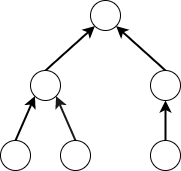
\includegraphics[width=0.8\linewidth]{GSSI_thesisProposal/figures/ina-2.png}
    \caption{An in-arborescence}
    \label{fig:ina}
\end{subfigure}
\hfill
\begin{subfigure}{0.4\textwidth}
    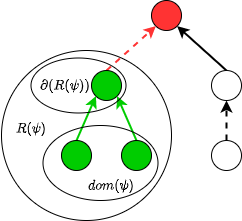
\includegraphics[width=0.8\linewidth]{GSSI_thesisProposal/figures/ina-1.png}
    \caption{Shrinking boundary of an in-arborescence}
    \label{fig:boundary}
\end{subfigure}
\caption{In-arborescence 
}
\label{fig:inar}
\end{figure}


\begin{theorem}\label{thrm1}
If $\mathcal{G}$ is the class of all the in-arborescences, then $$AG(\mathcal{G},k)\leq \frac{2}{1-(1-2/k)^k}\leq \frac{2e^2}{e^{2}-1}\approx 2.31,\ \forall k\geq 2.$$
\end{theorem}

Let $G=(V=[n],E,(p_{uv})_{(u,v)\in E})$ be an in-arborescence, where $n>k$ is the number of nodes. To show the claim of Theorem \ref{thrm1}, we need some preliminary notations and lemmas. Given a partial realization $\psi$, and a node $v\in V$, let 
$$\Delta(v|\psi):=\E_L[f(\psi\cup \{(v,R(\{v\},L))\})-f(\psi)|\psi\subseteq \phi_L],$$
i.e., $\Delta(v|\psi)$ is the expected increment of the influence spread due to node $v$ when the observed partial realization is $\psi$. We have the following claim (from \cite{Golovin2011a}), holding even for general graphs, whose proof is trivial. 

\begin{claim}[Adaptive Submodularity \cite{Golovin2011a}]\label{lem0}
Let $G$ be an arbitrary influence graph. For any partial realizations $\psi,\psi'$ of $G$ such that $\psi\subseteq \psi'$, and any node $v\notin R(\psi')$, we have that  $\Delta(v|\psi')\leq \Delta(v|\psi)$. 
\end{claim}


An adaptive policy $\pi$ is called {\em randomized} if, for any partial realization $\psi$, node $\pi(\psi)$ is not selected deterministically (in general), but randomly (according to a probability distribution $p_{\psi}$ depending on $\psi$). Given a vector $\bm y=(y_1,\ldots, y_n)$ such that $y_v\in [0,1]$ for any $v\in V$, we say that $\mathbb{P}(\pi)=\bm y$ if the probability that each node $v$ belongs to $dom(\psi_{\pi,L})$ is $y_v$, where $\psi_{\pi,L}$ is the partial realisation with policy $\pi$. Let $OPT_A(G,\bm y)$ be the optimal expected influence spread $\sigma(\pi)$ over all the randomized adaptive policies $\pi$ such that $\mathbb{P}(\pi)=\bm y$.\footnote{We observe that, if $\bm y$ is arbitrary, a deterministic policy $\pi$ verifying $\mathbb{P}(\pi)=\bm y$ might not exists, and the introduction of randomization solves this issue.}

Let $\pi^*$ be an optimal adaptive policy for the adaptive influence maximization problem (with $|\pi^*|=k$), and let $\bm x=(x_1,\ldots, x_n)$ be the vector such that $\mathbb{P}(\pi^*)=\bm x$. As $|\pi^*|=k$, we have that $\sum_{v\in V} x_v=k$. 

For any $t\in [k]_0$, let $S_t$ be the optimal set of $t$ seed nodes in the non-adaptive influence maximization problem, i.e., such that $OPT_N(G,t)=\mathbb{E}_L(|R(S_t,L)|)$. Let $\psi_{t,L}$ be the random variable denoting the sub-realisation of $\phi_L$ such that $dom(\psi_{t,L})=S_t$. Let $\rho$ be the random variable equal to node $v\in V$ with probability $x_v/k$. Observe that the above random variable is well-defined, as $\sum_{v\in V}(x_v/k)=k/k=1$. For any $t\in [k]$, let ${\psi}_{\rho,t,L}$ be the random variable denoting the sub-realisation of $\phi_L$ such that $dom({\psi}_{\rho,t,L})=S_{t-1}\cup\{\rho\}$.

\paragraph*{General outline of the proof technique} We observe that ${\psi}_{\rho,t,L}$ is the partial realization coming from the following  {\em hybrid non-adaptive policy}: initially, we activate the first $t-1$ seed nodes as in the optimal non-adaptive solution guaranteeing an expected influence spread of $OPT_N(G,t-1)$; then, we randomly choose a node $v$ according to random variable $\rho$ and we select $v$ as $t$-th seed node (if not already selected as seed). We use this hybrid non-adaptive policy as a main tool to obtain an improved upper bound on the adaptivity gap for in-arborescences. In Lemma \ref{lemm1}, holding even for general graphs, we relate the hybrid non-adaptive policy and the optimal non-adaptive solution, with the optimal adaptive policy. Lemma \ref{lemm1}, together with Lemma \ref{lemm2} (that is similar to Lemma 3.8 in~\cite{Chen2019}), is used in the main proof of the theorem to relate $OPT_N(G,t)$ with $OPT_A(G,k)$ for any $t\in [k]$, and this leads to our upper bound. 

The proof structure of Lemma \ref{lemm1} exhibits some similarities with Lemma 6 of \cite{Asadpour16} and Lemma 3.3 of \cite{Chen2019}, but in their approach, they relate non-adaptive policies based on the Poisson process and multi-linear extensions, with the optimal adaptive policy. One disadvantage of the Poisson process adopted in \cite{Chen2019} is that the number $X$ of seed nodes selected by the corresponding non-adaptive policy is equal to $k$ under expectation (i.e., $\mathbb{E}(X)=k$), and determining the expected influence spread w.r.t. random variable $X$ has implied a further loss in the final upper bound (see Lemma 3.9 and inequality (21) of Theorem 3.1 in \cite{Chen2019}). Instead, by using the hybrid-non-adaptive policy, we guarantee that the number of selected seed nodes at each step $t\in [k]$ is exactly equal to $t$,  independently from the considered random execution. This property allow us to avoid the expectations w.r.t. the number of selected seed nodes, and this leads to a further improvement of the resulting upper bound on the adaptivity gap.
\begin{lemma}\label{lemm1}
Let $G$ be an arbitrary influence graph. For any $t\in [k]$, and any fixed partial realization $\psi$ of $G$ such that $\mathbb{P}[\psi_{t-1,L}=\psi]>0$, we have $$OPT_A(G,k)\leq 
\sigma(R(\psi))+k\cdot \E_{L,\rho}\left[f({\psi}_{\rho,t,L})-f(\psi_{t-1,L})|\psi_{t-1,L}=\psi\right].$$
\end{lemma}
\begin{proof}
We have 
\begin{align}
&k\cdot \E_{L,\rho}\left[f({\psi}_{\rho,t,L})-f(\psi_{t-1,L})|\psi_{t-1,L}=\psi \right]\nonumber\\
=&k\cdot \sum_{v\in V}\mathbb{P}[\rho=v]\cdot \Delta(v|\psi)\nonumber\\
=&k\cdot \sum_{v\in V\setminus R(\psi)}\frac{x_v}{k}\cdot \Delta(v|\psi)\label{eq0}\\
=&\sum_{v\in V\setminus R(\psi)}x_v\cdot \Delta(v|\psi),\label{eq1}
\end{align}
where \eqref{eq0} holds since $\Delta(v|\psi)=0$ for any $v\in R(\psi)$. 

Let $\bm x'=(x_1',\ldots x_n')$ be the vector such that $x_v'=1$ if $v\in R(\psi)$, and $x_v'=x_v$ otherwise. As $x_v'\geq x_v$ for any $v\in V$ we have  
\begin{equation}\label{eq2}
OPT_A(G,k)\leq OPT_A(G,\bm x)\leq OPT_A(G,\bm x').
\end{equation}

Let $\pi'$ be the optimal randomized adaptive policy such that $\mathbb{P}(\pi')=\bm x'$. Policy $\pi'$ selects each node in $R(\psi)$ with probability $1$, thus we can assume that such seed nodes are selected at the beginning and that the adaptive policy starts by observing the resulting partial realization. Furthermore, we can assume that, for any partial realization $\psi'$, $\pi'$ does not select any node $v\in R(\psi')$, otherwise there is no increase of the influence spread. Given $j\in [n]$, let $\Delta'(j)$ denote the expected increment of the influence spread when $\pi'$ selects the $j$-th seed node (in order of selection, and without considering in the count the initial seeds of $R(\psi)$); analogously, let $\Delta'(j|v)$ denote the expected increment of the influence spread when $\pi'$ selects the $j$-th seed node, conditioned by the fact that the $j$-th seed is node $v$.\footnote{If an execution of $\pi'$ requires less than $j$ steps, we assume that the increase of the influence spread at step $j$ (that contributes to the expected values $\Delta'(j)$ and $\Delta'(j|v)$) is null.} We get
\begin{align}
 &OPT_A(G,\bm x')\nonumber\\
  =&\sigma(R(\psi))+\sum_j \Delta'(j)\nonumber\\
  =&\sigma(R(\psi))+\sum_j \sum_{v\in V\setminus R(\psi)}\mathbb{P}[\text{the $j$-th seed node is $v$}]\cdot \Delta'(j|v)\nonumber\\
  =&\sigma(R(\psi))+\sum_{v\in V\setminus R(\psi)}\sum_j \mathbb{P}[\text{the $j$-th seed node is $v$}]\cdot \Delta'(j|v)\nonumber\\
    =&\sigma(R(\psi))+\sum_{v\in V\setminus R(\psi)}\sum_j \mathbb{P}[\text{the $j$-th seed node is $v$}]\cdot\nonumber\\
    \cdot & \E_{\pi'}[\Delta(v|\psi')|\text{$v=\pi'(\psi')$ for some $\psi'\supseteq \psi$ observed at step $j$}]\nonumber\\
        \leq &\sigma(R(\psi))+\sum_{v\in V\setminus R(\psi)}\sum_j \mathbb{P}[\text{the $j$-th seed node is $v$}]\cdot \Delta(v|\psi)\label{eq3.0}\\
                =&\sigma(R(\psi))+\sum_{v\in V\setminus R(\psi)}\mathbb{P}[\text{$v$ is selected as seed}]\cdot \Delta(v|\psi)\nonumber\\
=& \sigma(R(\psi))+\sum_{v\in V\setminus R(\psi)}x_v'\cdot \Delta(v|\psi)\nonumber\\
= & \sigma(R(\psi))+\sum_{v\in V\setminus R(\psi)}x_v\cdot \Delta(v|\psi),\label{eq3}
\end{align}
where \eqref{eq3.0} holds since $\Delta(v|\psi')\leq \Delta(v|\psi)$ for any partial realization $\psi'\supseteq \psi$ by adaptive submodularity (Claim \ref{lem0}). By putting together \eqref{eq1}, \eqref{eq2}, and \eqref{eq3}, we get
\begin{align*}
& \sigma(R(\psi))+k\cdot \E_{L,\rho}\left[f({\psi}_{\rho,t,L})-f(\psi_{t-1,L})|\psi_{t-1,L}=\psi \right]\\
=& \sigma(R(\psi))+\sum_{v\in V\setminus R(\psi)}x_v\cdot \Delta(v|\psi)\\
\geq & OPT_A(G,\bm x')\\
\geq & OPT_A(G,k),
\end{align*}
thus showing the claim. 
\end{proof}

\begin{lemma}\label{lemm2}
If the input influence graph $G$ is an in-arborescence, then $$
\sigma(R(\psi_{t-1,L}))\leq f(\psi_{t-1,L})+OPT_N(G,t-1)$$
  for any live-edge graph $L$ and $t\in [k]$. 
\end{lemma}
\begin{proof}
Given a subset $U\subseteq V$, let $\partial U:=\{u\in U:\exists (u,v)\in E,v\notin U\}$. We have that $\sigma(R(\psi))\leq |R(\psi)|+\sigma(\partial R(\psi))=f(\psi)+\sigma(\partial R(\psi))$ for any partial realization $\psi$. Thus, to show the claim, it suffices to show that $\sigma(\partial R(\psi_{t-1,L}))\leq OPT_N(G,t-1)$. For in-arborescences, we have that $|\partial R(\psi_{t-1,L})|\leq |dom(\psi_{t-1,L})|=t-1$, thus $\sigma(\partial R(\psi_{t-1,L}))\leq OPT_N(G,t-1)$.
\end{proof}
Armed with the above lemmas, we can now prove Theorem~\ref{thrm1}.

\begin{proof}[Proof of Theorem~\ref{thrm1}]
For any $t\in [k]$, we have
\begin{align}
&k\cdot (OPT_N(G,t)-OPT_N(G,t-1))\nonumber\\
=&k\cdot (\sigma(S_t)-\sigma(S_{t-1}))\nonumber\\
=&k\cdot (\E_L[f(\psi_{t,L})]-\E_L[f(\psi_{t-1,L})])\nonumber\\
\geq &k\cdot (\E_{L,\rho}[f({\psi}_{\rho,t,L})]-\E_L[f(\psi_{t-1,L})])\label{eqthm1.0}\\
= &k\cdot (\E_{L,\rho}[f({\psi}_{\rho,t,L})]-\E_{L,\rho}[f(\psi_{t-1,L})])\nonumber\\
=&k\cdot \E_{L,\rho}[f({\psi}_{\rho,t,L})-f(\psi_{t-1,L})]\nonumber\\
=& \E_{\psi_{t-1,L}}\left[k\cdot \E_{L,\rho}[f({\psi}_{\rho,t,L})-f(\psi_{t-1,L})|\psi_{t-1,L}]\right]\nonumber\\
\geq &\E_{\psi_{t-1,L}}[OPT_A(G,k)-\sigma(R(\psi_{t-1,L}))]\label{eqthm1}\\
\geq &\E_{\psi_{t-1,L}}[OPT_A(G,k)-f(\psi_{t-1,L})-OPT_N(G,t-1)]\label{eqthm3}\\
=& \E_{\psi_{t-1,L}}[OPT_A(G,k)]-\E_{\psi_{t-1,L}}[f(\psi_{t-1,L})]-\E_{\psi_{t-1,L}}[OPT_N(G,t-1)]\nonumber\\
= &OPT_A(G,k)-\sigma(S_{t-1})-OPT_N(G,t-1)\nonumber\\
= &OPT_A(G,k)-2\cdot OPT_N(G,t-1)\label{eqthm4},
\end{align}
where \eqref{eqthm1.0} holds since $dom(\psi_{t,L})$ is the optimal set of $t$ seed nodes for the non-adaptive influence maximization problem, \eqref{eqthm1} comes from Lemma \ref{lemm1}, and \eqref{eqthm3} comes from Lemma~\ref{lemm2}. Thus, by \eqref{eqthm4}, we get $k\cdot (OPT_N(G,t)-OPT_N(G,t-1))\geq OPT_A(G,k)-2\cdot OPT_N(G,t-1)$, that after some manipulations leads to the following recursive relation:
\begin{equation}
OPT_N(G,t)\geq \frac{1}{k}\cdot OPT_A(G,k)+\left(1-\frac{2}{k}\right)\cdot OPT_N(G,t-1),\ \forall t\in [k].\label{fundeqthm}
\end{equation}
%
By applying \eqref{fundeqthm} iteratively, we get
\begin{align*}
    OPT_N(G,k)&\geq \frac{1}{k}\cdot \sum_{t=0}^{k-1}\left(1-\frac{2}{k}\right)^{t}\cdot OPT_A(G,k)=\frac{1-\left(1-2/k\right)^k}{2}\cdot OPT_A(G,k),
\end{align*}
that leads to 
\begin{equation*}
\frac{OPT_A(G,k)}{OPT_N(G,k)}\leq \frac{2}{1-(1-2/k)^k}\leq \frac{2}{1-e^{-2}} = \frac{2e^2}{e^{2}-1},
\end{equation*}
and this shows the claim. 
\end{proof}
\section{Adaptivity Gap for General Influence  Graphs}\label{sec_gen}
In this section, we exhibit upper bounds on the $k$-adaptivity gap of general graphs. In the following theorem, we first give an upper bound that is linear in the number of seed nodes.
\begin{theorem}\label{lemk}
Given an arbitrary class of influence graphs $\mathcal{G}$ and $k\geq 2$, we get $AG(\mathcal{G},k)\leq k$. 
\end{theorem}
\begin{proof}
Let $G=(V=[n],E,(p_{uv})_{(u,v)\in E})$ be an arbitrary influence graph. Let $\pi^*$ be an optimal adaptive policy subject to $|\pi^*|=k$, and let $\psi_{t,\pi^*,L}$ be the partial realization observed when the $t$-th seed node has been selected by Algorithm \ref{ad_alg} with policy $\pi^*$. Fix $t\in [k]$, a partial realization $\psi$ such that $\mathbb{P}[\psi_{t,\pi^*,L}=\psi]>0$, and let $v=\pi^*(\psi)$ be the node selected by policy $\pi^*$ under partial realization $\psi$. We have that
\begin{align}
&\E_{L}[f(\psi_{t,\pi^*,L})-f(\psi_{t-1,\pi^*,L})|\psi_{t-1,\pi^*,L}=\psi]\nonumber\\
=&\Delta(v|\psi)\nonumber\\
\leq & \Delta(v|\emptyset)\label{eq1lemk}\\
=&\sigma(\{v)\})\nonumber\\
\leq & OPT_N(G,1),\label{eq2lemk}
\end{align}
where \eqref{eq1lemk} holds by adaptive submodularity (Claim  \ref{lem0}). Thus, we get
\begin{align}
OPT_A(G,k)=&\E_{L}[f(\psi_{k,\pi^*,L})]\nonumber\\
=&\sum_{t=1}^k \E_{L}[f(\psi_{t,\pi^*,L})-f(\psi_{t-1,\pi^*,L})]\nonumber\\
=&\sum_{t=1}^k \E_{\psi_{t-1,\pi^*,L}}[\E_L[f(\psi_{t,\pi^*,L})-f(\psi_{t-1,\pi^*,L})|\psi_{t-1,\pi^*,L}]]\nonumber\\
\leq &k\cdot\E_{\psi_{t-1,\pi^*,L}}[OPT_N(G,1)]\label{eq3lemk}\\
=&k\cdot OPT_N(G,1)\nonumber\\
\leq &k\cdot OPT_N(G,k),
\end{align}
where \eqref{eq3lemk} comes from \eqref{eq2lemk}, and the claim follows.
\end{proof}
In the next theorem we give an upper bound on the adaptivity gap that is sublinear in the number of nodes of the considered graph.

When considering general graphs having a bounded number of nodes, we get an upper bound on the adaptivity gap that is sublinear in the maximum number of nodes of the considered graphs. 

\begin{theorem}\label{thrm2}
If $\mathcal{G}$ is the class of influence graphs having at most $n$ nodes, we get $AG(\mathcal{G})\leq \lceil n^{1/3}\rceil .$ 
\end{theorem}

Let $G=(V,E,(p_{uv})_{(u,v)\in E})$ be the input influence graph. To show Theorem \ref{thrm2}, we recall the preliminary notations considered for the proof of Theorem \ref{thrm1}, and we give a further preliminary lemma. 
\begin{lemma}\label{lemthm2}
Given a set $U\subseteq V$ of cardinality $h\geq k$, we have $\sigma(U)\leq \frac{h}{k}\cdot OPT_N(G,k).$
\end{lemma}
\begin{proof}
For any $t\in [h]_0$, let $U_t:=\emptyset$ if $t=0$, and $U_t:=U_{t-1}\cup\{v_t\}$, where $v_t\in\arg\max_{v\in U\setminus U_{t-1}}(\sigma(U_{t-1}\cup\{v\})-\sigma(U_{t-1})).$ We have that $\Delta_t:=\sigma(U_{t})-\sigma(U_{t-1})$ is non-increasing in $t\in [h]$. Indeed, given $t\in [k-1]$, we have that
\begin{align}
\Delta_{t+1}=&\sigma(U_{t+1})-\sigma(U_{t})\nonumber\\
=&\sigma(U_{t}\cup\{v_{t+1}\})-\sigma(U_{t})\nonumber\\
\leq &\sigma(U_{t-1}\cup\{v_{t+1}\})-\sigma(U_{t-1})\label{eq1lem2thm2}\\
\leq &\max_{v\in U\setminus U_{t-1}}(\sigma(U_{t-1}\cup\{v\})-\sigma(U_{t-1}))\nonumber\\
=&\sigma(U_{t-1}\cup\{v_{t}\})-\sigma(U_{t-1})\nonumber\\
=&\Delta_t,\label{eq2lem2thm2}
\end{align}
where \eqref{eq1lem2thm2} holds since $\sigma$ is a submodular set-function (see \cite{Kempe2015}). Thus, we necessarily have 
\begin{align}
\frac{\sigma(U)}{h}=&\frac{\sum_{t=1}^h\Delta_t}{h}\nonumber\\
\leq &\frac{\sum_{t=1}^k\Delta_t\left(h/k\right)}{h}\label{eq3lem2thm2}\\
=&\frac{\sum_{t=1}^k\Delta_t}{k}\nonumber\\
=&\frac{\sigma(U_k)}{k}\nonumber\\
\leq &\frac{OPT_N(G,k)}{k},\label{eq4lem2thm2}
\end{align}
where \eqref{eq3lem2thm2} comes from \eqref{eq2lem2thm2}. By \eqref{eq4lem2thm2}, the claim follows.
\end{proof}
We use Theorem~\ref{lemk} and Lemma~\ref{lemthm2} to show Theorem~\ref{thrm2}.

\begin{proof}[Proof of Theorem~\ref{thrm2}]
We assume w.l.o.g. that $k>\lceil n^{1/3}\rceil $ and that $OPT_N(G,k)<(\lceil n^{1/3}\rceil)^2$. Indeed, if $k\leq  \lceil n^{1/3}\rceil $, by Theorem \ref{lemk} the claim holds, and if $OPT_N(G,k)\geq (\lceil n^{1/3}\rceil)^2$, then $\frac{OPT_A(G,k)}{OPT_N(G,k)}\leq \frac{|V|}{OPT_N(G,k)}\leq \frac{n}{(\lceil n^{1/3}\rceil)^2}\leq \lceil n^{1/3}\rceil $, and the claim holds as well. 
For any $t\in [k]$, we have
\begin{align}
&k\cdot (OPT_N(G,t)-OPT_N(G,t-1))\nonumber\\
\geq &k\cdot (\E_{L,\rho}[f({\psi}_{\rho,t,L})]-\E_{L,\rho}[f(\psi_{t-1,L})])\nonumber\\
=& \E_{\psi_{t-1,L}}\left[k\cdot \E_{L,\rho}[f({\psi}_{\rho,t,L})-f(\psi_{t-1,L})|\psi_{t-1,L}]\right]\nonumber\\
\geq &\E_{\psi_{t-1,L}}[OPT_A(G,k)-\sigma(R(\psi_{t-1,L}))]\label{eqthm12}\\
=&\E_{\psi_{t-1,L}}[OPT_A(G,k)]-\E_{\psi_{t-1,L}}[\sigma(R(\psi_{t-1,L}))]\nonumber\\
\geq &\E_{\psi_{t-1,L}}[OPT_A(G,k)]-\E_{\psi_{k,L}}[\sigma(R(\psi_{k,L}))]\nonumber\\
\geq &\E_{\psi_{t-1,L}}[OPT_A(G,k)]-\E_{\psi_{k,L}}\left[\frac{|R(\psi_{k,L})|}{k}\cdot OPT_N(G,k)\right]\label{eqthm32}\\
= &OPT_A(G,k)-\frac{\E_{\psi_{k,L}}[|R(\psi_{k,L})|]}{k}\cdot OPT_N(G,k)\nonumber\\
\geq  &OPT_A(G,k)-\frac{\E_{\psi_{k,L}}[|R(\psi_{k,L})|]}{\lceil n^{1/3}\rceil+1}\cdot ((\lceil n^{1/3}\rceil)^2-1)\label{eqthm42}\\
=&OPT_A(G,k)-(\lceil n^{1/3}\rceil-1)\cdot \E_{\psi_{k,L}}[|R(\psi_{k,L})|]\nonumber\\
=&OPT_A(G,k)-(\lceil n^{1/3}\rceil-1)\cdot OPT_N(G,k)\label{eqthm52},
\end{align}
where \eqref{eqthm12} comes from Lemma \ref{lemm1}, \eqref{eqthm32} comes from Lemma \ref{lemthm2}, and \eqref{eqthm42} comes from the hypothesis $k>\lceil n^{1/3}\rceil $ and $OPT_N(G,k)<(\lceil n^{1/3}\rceil)^2$. By \eqref{eqthm52}, we get $OPT_N(G,t)-OPT_N(G,t-1)
\geq (OPT_A(G,k)-(\lceil n^{1/3}\rceil-1)\cdot OPT_N(G,k))/k$ for any $t\in [k]$, and by summing such inequality over all $t\in [k]$, we get
\begin{align}
& OPT_N(G,k)\nonumber\\
=&\sum_{t=1}^k (OPT_N(G,t)-OPT_N(G,t-1))\nonumber\\
\geq &\sum_{t=1}^k\frac{OPT_A(G,k)-(\lceil n^{1/3}\rceil-1)\cdot OPT_N(G,k)}{k}\nonumber\\
=&OPT_A(G,k)-(\lceil n^{1/3}\rceil-1)\cdot OPT_N(G,k).\label{eqthm62}
\end{align}
Finally, \eqref{eqthm62} implies that $OPT_A(G,k)\leq \lceil n^{1/3}\rceil \cdot OPT_N(G,k)$, and this shows the claim. 
\end{proof}
\section{Adaptivity Gap for Other Influence Graphs}\label{sec_other}
In this section, we extend the results obtained in Theorem \ref{thrm1}, and we get upper bounds on the adaptivity gap of other classes of influence graphs. 
\subsection {$\alpha$-bounded-degree graphs} \label{sec_alpha}
We first consider the class of {\em $\alpha$-bounded-degree graphs}: a class of undirected influence graphs parametrized by an integer $\alpha\geq 0$ that includes several known graph topologies. In the following, when we refer to undirected influence graphs, we assume that, for any undirected edge $\{u,v\}$, there are two directed edges $(u,v)$ and $(v,u)$ having respectively two (possibly) distinct probabilities $p_{uv}$ and $p_{vu}$. 

Given an undirected graph $G=(V,E)$ and a node $v\in V$, let $deg_v(G)$ denote the degree of node $v$ in graph $G$. Given an integer $\alpha\geq 0$, an influence graph $G=(V,E,(p_{uv})_{(u,v)\in E})$ is an {\em $\alpha$-bounded-degree graph} if it is undirected and $\sum_{v\in V:deg_v(G)>2}deg_v(G)\leq \alpha,$ i.e., the sum all the node degrees higher than $2$ is at most $\alpha$; we observe that the definition of $\alpha$-bounded degree graphs does not depends on the influence probabilities, but on the graph topology only. 
\begin{example}\label{exam1}
Given an undirected graph $G$, a simple subpath $P$ (resp. cycle $C$) of $G$ is {\em standard} if all the nodes of $P$ but the first and the last one (resp. all the nodes of $C$) have degree $2$. The {\em standard contraction} of $G$ is the multigraph $G'$ obtained by replacing each maximal simple subpath $P=(v_1,\ldots, v_t)$ of $G$ such that $deg_{v_2}(G)=deg_{v_3}(G)=deg_{v_{t-1}}(G)=2$, with an edge and by deleting each simple cycle $C=(v_1,v_2,\ldots, v_{t-1},v_t=v_1)$ such that $deg_{v_2}(G)=deg_{v_3}(G)=deg_{v_{t-1}}(G)=2$. There are several interesting classes of $\alpha$-bounded-degree graphs characterized by the topological structure of their standard contraction:
\begin{itemize}
\item The set of $0$-bounded-degree graphs is made of all the graphs $G$ such that each connected component of $G$ is either an undirected path or an undirected cycle; equivalently, the set of $0$-bounded-degree graphs is made of all the graphs $G$ whose standard contraction is the (possibly empty) union of several disconnected edges.
\item If the standard contraction of a graph $G$ is homeomorphic to a star with $h$ edges, then $G$ is a $h$-bounded-degree graph.
\item If the standard contraction of a graph $G$ is homeomorphic to a parallel-link multigraph with $h$ edges, then $G$ is a $2h$-bounded-degree graph.
\item If the standard contraction of a graph $G$ is homeomorphic to a cycle with $h$ chords, then $G$ is a $6h$-bounded-degree graph.
\item If the standard contraction of a graph $G$ is homeomorphic to a clique with $h$ nodes, then $G$ is a $h(h-1)$-bounded-degree graph.
\end{itemize}
\end{example}
In the following, we provide an upper bound on the adaptivity gap of $\alpha$-bounded-degree graphs for any $\alpha\geq 0$. 
\begin{theorem}\label{thmlast}
Given $\alpha\geq 0$, let $\mathcal{G}$ be the class of  $\alpha$-bounded-degree graphs. Then 
$$AG(\mathcal{G},k)\leq \min\left\{k,\frac{\alpha}{k}+2+ \frac{1}{1-(1-1/k)^k}\right\}\leq \frac{\sqrt{4(e-1)^2\alpha+(3e-2)^2}+3e-2}{2(e-1)}$$
for any $k\geq 2$, i.e., $AG(\mathcal{G})\leq \sqrt{\alpha}+O(1)$. 
\end{theorem}

Let $G=(V=[n],E,(p_{uv})_{(u,v)\in E})$ be an $\alpha$-bounded-degree graph, and we recall the preliminary notations from Theorem \ref{thrm1}. The proof of Theorem \ref{thmlast} is a non-trivial generalization of Theorem \ref{thrm1}. In particular, the proof resorts to Theorem \ref{lemk} to get the upper bound of $k$, and, by following the approach of Theorem \ref{thrm1}, the following technical lemma is used in place of Lemma \ref{lemm2} to get the final upper bound. 
\begin{lemma}\label{lemlast}
When the input influence graph $G$ is an $\alpha$-bounded-degree graph with $\alpha\geq 0$, we have that $
\sigma(R(\psi_{t-1,L}))\leq f(\psi_{t-1,L})+\left(\frac{\alpha}{k}+2\right)\cdot OPT_N(G,k)$ for any $t\in [k]$ and live-edge graph $L$.
\end{lemma}
\begin{proof}%[Proof of Lemma \ref{lemlast}]
Given a subset $U\subseteq V$, let $\partial U:=\{u\in U: \exists (u,v)\in E,v\notin U\}$. We have that $\sigma(R(\psi))\leq |R(\psi)|+\sigma(\partial R(\psi))=f(\psi)+\sigma(\partial R(\psi))$ for any partial realization $\psi$. Thus, to show the claim, it suffices to show that 
\begin{equation*}%\label{eqlast1}
\sigma(\partial R(\psi_{t-1,L}))\leq \left(\frac{\alpha}{k}+2\right)\cdot OPT_N(G,k).
\end{equation*}
Let $U\subseteq V$ such that $U$ has at most $k$ connected components. Let $A$ be the set of connected components containing at least one node of degree higher than $2$, and let $B$ be the set of the remaining components, i.e., containing nodes with degree in $[2]_0$ only. By definition of $A$ and $B$, we necessarily have that $|\partial A|\leq \sum_{v\in V:deg_v(G)>2}deg_v(G)\leq \alpha$ and $|\partial B|\leq 2k$. Thus $|\partial U|\leq |\partial A|+|\partial B|\leq \alpha+2k$, and the next claim follows.
\begin{claim}\label{lastclaim}
Given a subset $U\subseteq V$ made of at most $k$ connected components, then $|\partial U|\leq \alpha+2k$. 
\end{claim}
Now, we have that
\begin{align}
\sigma(\partial R(\psi_{t-1,L}))\leq & \sigma(\partial R(\psi_{k,L}))\nonumber\\
\leq & \frac{|\partial R(\psi_{k,L})|}{k}\cdot OPT_N(G,k)\label{lastlem_eq2}\\
\leq & \frac{\alpha+2k}{k}\cdot OPT_N(G,k),\label{lastlem_eq3}
\end{align}
where \eqref{lastlem_eq2} comes from Lemma \ref{lemthm2}, and \eqref{lastlem_eq3} holds since $R(\psi_{k,L})$ contains at most $k$ connected components and because of Claim \ref{lastclaim}. Thus, by \eqref{lastlem_eq3}, the claim of the lemma follows. 
\end{proof}

We can now prove Theorem~\ref{thmlast}.
\begin{proof}[Proof of Theorem~\ref{thmlast}]
For any $t\in [k]$, we have
\begin{align}
&k\cdot (OPT_N(G,t)-OPT_N(G,t-1))\nonumber\\
\geq &k\cdot (\E_{L,\rho}[f({\psi}_{\rho,t,L})]-\E_{L,\rho}[f(\psi_{t-1,L})])\nonumber\\
=& \E_{\psi_{t-1,L}}\left[k\cdot \E_{L,\rho}[f({\psi}_{\rho,t,L})-f(\psi_{t-1,L})|\psi_{t-1,L}]\right]\nonumber\\
\geq &\E_{\psi_{t-1,L}}[OPT_A(G,k)-\sigma(R(\psi_{t-1,L}))]\label{eqthm1_last}\\
\geq &\E_{\psi_{t-1,L}}\left[OPT_A(G,k)-f(\psi_{t-1,L})-\left(\frac{\alpha}{k}+2\right)OPT_N(G,k)\right]\label{eqthm3_last}\\
=& \E_{\psi_{t-1,L}}[OPT_A(G,k)]-\E_{\psi_{t-1,L}}[f(\psi_{t-1,L})]-\left(\frac{\alpha}{k}+2\right)\cdot\E_{\psi_{t-1,L}}\left[OPT_N(G,k)\right]\nonumber\\
= &OPT_A(G,k)-\sigma(S_{t-1})-\left(\frac{\alpha}{k}+2\right)\cdot OPT_N(G,k)\nonumber\\
= &OPT_A(G,k)-\left(\frac{\alpha}{k}+2\right)\cdot OPT_N(G,k)-OPT_N(G,t-1)\label{eqthm4_last},
\end{align}
where \eqref{eqthm1_last} comes from Lemma \ref{lemm1} and \eqref{eqthm3_last} comes from Lemma \ref{lemlast}. Thus, by \eqref{eqthm4_last}, we get the following recursive relation:
\begin{equation}\label{fundeqthm_last}
OPT_N(G,t)\geq \frac{1}{k}\left(OPT_A(G,k)-\left(\frac{\alpha}{k}+2\right)OPT_N(G,k)\right)+\left(1-\frac{1}{k}\right)OPT_N(G,t-1),
\end{equation}
for any $t\in [k]$. By applying iteratively \eqref{fundeqthm_last}, we get 
\begin{align*}
OPT_N(G,k)
&\geq \frac{1}{k}\cdot \left(OPT_A(G,k)-\left(\frac{\alpha}{k}+2\right)\cdot OPT_N(G,k)\right)\cdot \sum_{t=0}^{k-1} \left(1-\frac{1}{k}\right)^j\\
&=\left(OPT_A(G,k)-\left(\frac{\alpha}{k}+2\right)\cdot OPT_N(G,k)\right)\cdot \left(1-\left(1-\frac{1}{k}\right)^k\right),
\end{align*}
that, after some manipulations, leads to 
\begin{equation}\label{semifinal_bound}
%\frac{OPT_A(G,k)}{OPT_N(G,k)}\leq \frac{(\alpha/k+2)(1-(1-1/k)^k)+1}{1-(1-1/k)^k}.
\frac{OPT_A(G,k)}{OPT_N(G,k)}\leq \frac{\alpha}{k}+2+ \frac{1}{1-(1-1/k)^k} \leq \frac{\alpha}{k}+2+ \frac{1}{1-e^{-1}}~.
\end{equation}
By Theorem \ref{lemk}, we have that $\frac{OPT_A(G,k)}{OPT_N(G,k)}\leq k$, thus, by \eqref{semifinal_bound}, we get 
\begin{align}
\frac{OPT_A(G,k)}{OPT_N(G,k)}\leq & \min\left\{k, \frac{\alpha}{k}+2+ \frac{1}{1-(1-1/k)^k} \  \right\}\nonumber\\
\leq & \min\left\{k, \frac{\alpha}{k}+2+ \frac{1}{1-e^{-1}} \  \right\}\nonumber\\
\leq  & \frac{\sqrt{4(e-1)^2\alpha+(3e-2)^2}+3e-2}{2(e-1)}\label{last_eqq},
\end{align}
where \eqref{last_eqq} is equal to the real value of $k\geq 0$ such that $k=\frac{\alpha}{k}+2+ \frac{1}{1-e^{-1}}$. By \eqref{last_eqq} the claim follows. 
\end{proof}

For the particular case of $0$-bounded-degree graphs, the following theorem provides a better  upper bound on the adaptivity gap.
\begin{theorem}\label{thm_0bou}
Let $\mathcal{G}$ be the class of $0$-bounded-degree graphs. Then $$AG(\mathcal{G},k)\leq\min\left\{k,\frac{3}{1-(\max\{0,1-3/k\})^k}\right\}\leq \frac{3e^3}{e^{3}-1}\approx 3.16,$$ 
for any $k\geq 2$. 
\end{theorem}
The proof of Theorem \ref{thm_0bou} is similar to that of Theorem \ref{thrm1}. Let $G=(V=[n],E,(p_{uv})_{(u,v)\in E})$ be a $0$-bounded-degree graph. We recall the notation from Theorem \ref{thrm1} and we give the following preliminary lemma, whose proof is analogue to that of Lemma \ref{lem2}. 
\begin{lemma}\label{lem_0bou}
When the input influence graph $G$ is a $0$-bounded-degree graph, we have  
\begin{equation}
\sigma(R(\psi_{t-1,L}))\leq f(\psi_{t-1,L})+2\cdot OPT_N(G,t-1),
\end{equation}
for any $t\in [k]$ and live-edge graph $L$.
\end{lemma}
\begin{proof}
As in Lemma \ref{lemm2}, we show that $\sigma(\partial R(\psi_{t-1,L}))\leq 2\cdot OPT_N(G,t-1)$. First of all, we assume that $t\geq 2$, otherwise $\sigma(R(\psi_{t-1,L}))$ and the claim holds. By Lemma \ref{lemthm2}, we have that $\sigma(\partial R(\psi_{t-1,L}))\leq \frac{|\partial R(\psi_{t-1,L})|}{t-1}\cdot OPT_N(G,t-1)$. As $G$ is a $0$-bounded-degree graph, we have that $|\partial R(\psi_{t-1,L})|\leq 2(t-1)$. By considering the above  inequalities, we get $\sigma(\partial R(\psi_{t-1,L}))\leq \frac{|\partial R(\psi_{t-1,L})|}{t-1}\cdot OPT_N(G,t-1)\leq \frac{2(t-1)}{t-1}\cdot OPT_N(G,t-1)=2\cdot OPT_N(G,t-1)$, and the claim follows. 
\end{proof}
We are now ready to show Theorem \ref{thm_0bou}. 
\begin{proof}[Proof of Theorem \ref{thm_0bou}] By Theorem \ref{lemk}, we have that $k$ is an upper bound on the $k$-adaptivity gap, thus it is sufficient showing that $\frac{3}{1-(\max\{0,1-3/k\})^k}$ is a further upper bound.  If $k\leq 3$ the claim trivially holds, since $k$ is an upper bound on the $k$-adaptivity gap. Then, we assume that $k>3$, and it is sufficient showing that $\frac{3}{1-(1-3/k)^k}$ is an upper bound. For any $t\in [k]$, we have
\begin{align}
&k\cdot (OPT_N(G,t)-OPT_N(G,t-1))\nonumber\\
=&k\cdot (\sigma(S_t)-\sigma(S_{t-1}))\nonumber\\
=&k\cdot (\E_L[f(\psi_{t,L})]-\E_L[f(\psi_{t-1,L})])\nonumber\\
\geq &k\cdot (\E_{L,\rho}[f({\psi}_{\rho,t,L})]-\E_L[f(\psi_{t-1,L})])\nonumber\\
= &k\cdot (\E_{L,\rho}[f({\psi}_{\rho,t,L})]-\E_{L,\rho}[f(\psi_{t-1,L})])\nonumber\\
=&k\cdot \E_{L,\rho}[f({\psi}_{\rho,t,L})-f(\psi_{t-1,L})]\nonumber\\
=& \E_{\psi_{t-1,L}}\left[k\cdot \E_{L,\rho}[f({\psi}_{\rho,t,L})-f(\psi_{t-1,L})|\psi_{t-1,L}]\right]\nonumber\\
\geq &\E_{\psi_{t-1,L}}[OPT_A(G,k)-\sigma(R(\psi_{t-1,L}))]\label{eqthm1_0bou}\\
\geq &\E_{\psi_{t-1,L}}[OPT_A(G,k)-f(\psi_{t-1,L})-2\cdot OPT_N(G,t-1)]\label{eqthm3_0bou}\\
=& \E_{\psi_{t-1,L}}[OPT_A(G,k)]-\E_{\psi_{t-1,L}}[f(\psi_{t-1,L})]-2\cdot\E_{\psi_{t-1,L}}[OPT_N(G,t-1)]\nonumber\\
= &OPT_A(G,k)-\sigma(S_{t-1})-2\cdot OPT_N(G,t-1)\nonumber\\
= &OPT_A(G,k)-3\cdot OPT_N(G,t-1)\label{eqthm4_0bou},
\end{align}
where \eqref{eqthm1_0bou} comes from Lemma \ref{lemm1} and \eqref{eqthm3_0bou} comes from Lemma \ref{lem_0bou}. Thus, by \eqref{eqthm4_0bou}, we get $k\cdot (OPT_N(G,t)-OPT_N(G,t-1))\geq OPT_A(G,k)-3\cdot OPT_N(G,t-1)$, that after some manipulations leads to the following recursive relation:
\begin{equation}\label{fundeqthm_0bou}
OPT_N(G,t)\geq \frac{1}{k}\cdot OPT_A(G,k)+\left(1-\frac{3}{k}\right)\cdot OPT_N(G,t-1),\ \forall t\in [k].
\end{equation}
By applying iteratively \eqref{fundeqthm_0bou}, we get
\begin{equation*}
OPT_N(G,k)\geq \frac{1}{k}\cdot \sum_{t=0}^{k-1}\left(1-\frac{3}{k}\right)^{t}\cdot OPT_A(G,k)=\frac{1-\left(1-3/k\right)^k}{3}\cdot OPT_A(G,k),
\end{equation*}
that leads to 
\begin{equation}
\frac{OPT_A(G,k)}{OPT_N(G,k)}\leq \frac{3}{1-(1-3/k)^k}\leq \frac{3}{1-e^{-3}},
\end{equation}
and this shows the claim.
\end{proof}
\subsection{$(\beta,\gamma)$-bounded-activation graphs} \label{sec:beta}
Let $N(u):=\{v\in V:(u,v)\in E\}$ denote the set of out-neighbors of node $u$. Given an integer $\beta\geq 0$ and a real value $\gamma\in [0,1)$, an influence graph $G=(V,E,(p_{uv})_{(u,v)\in E})$ is a {\em $(\beta,\gamma)$-bounded-activation graph} if there exists $\hat{S}\subseteq V$ with $|\hat{S}|\leq \beta$ such that $\sum_{v\in N(u)}p_{u,v}\leq \gamma$ for any $u\in V\setminus \hat{S}$. Informally, the class of $(\beta,\gamma)$-bounded-activation graphs coincides with all the influence graphs such that all nodes but $\beta$ influence in expectation has at most $\gamma$ neighbors each.

In the following theorem, whose proof is partially based on Theorem \ref{lemk} and Lemma~\ref{lemthm2}, we provide an upper bound on the adaptivity gap of $(\beta,\gamma)$-bounded-activation graphs, for any integer $\beta\geq 0$ and $\gamma\in [0,1)$.
\begin{theorem}\label{thmlast2}
Given an integer $\beta\geq 0$ and $\gamma\in [0,1)$, let $\mathcal{G}$ be the class of $(\beta,\gamma)$-bounded-activation graphs. Then 
\begin{align}
AG(\mathcal{G},k)&\leq \min\left\{k,\frac{\max\{\beta,k\}\cdot \min\{1,\beta\}+\frac{k}{1-\gamma}}{k}\right\}\label{beta1}\\
&\leq \max\left\{\frac{\sqrt{\left(\frac{1}{1-\gamma}\right)^2+4\beta}+\frac{1}{1-\gamma}}{2},\min\{1,\beta\}+\frac{1}{1-\gamma}\right\}\nonumber\\
&\leq \sqrt{\beta}+\frac{1}{1-\gamma}.\nonumber
\end{align}
for any $k\geq 2$.
\end{theorem}
Let $G=(V=[n],E,(p_{uv})_{(u,v)\in E})$ be a $(\beta,\gamma)$-bounded-activation graph. To show the claim of Theorem \ref{thmlast2}, we recall the notations from Theorem \ref{thrm1} and we give some preliminary lemmas. 

Let $\hat{S}$ be the set of nodes such that $|\hat{S}|\leq \beta$ and $\sum_{v\in N(u)}p_{u,v}\leq \gamma$ for any $u\in V\setminus \hat{S}$. Let $G\setminus \hat{S}$ be the graph obtained from $G$ by removing the nodes in $\hat{S}$ and their adjacent edges, and let $OPT_N(G\setminus \hat{S},1)$ denote the optimal non-adaptive influence spread $OPT_N(G\setminus \hat{S},1)$ achieved by a unique seed in graph $G\setminus \hat{S}$. In the following lemma, we provide an upper bound for the optimal adaptive influence spread $OPT_A(G,k)$ in $G$.
\begin{lemma}\label{lemlast1}
We have that $OPT_A(G,k)\leq \sigma(\hat{S})+k\cdot OPT_N(G\setminus \hat{S},1).$
\end{lemma}
\begin{proof}
Let $\hat{\pi}$ be an optimal adaptive policy that first selects the nodes in $\hat{S}$ and then adaptively selects $k$ nodes. By construction, we have that 
\begin{equation}\label{lemlast1_eq1}
OPT_A(G,k)\leq \sigma(\hat{\pi}).
\end{equation}
Let $\psi_{0,\hat{\pi},L}$ denote the partial realization observed by $\hat{\pi}$ after the selection of $\hat{S}$, and let $\psi_{t,\hat{\pi},L}$ be the partial realization observed after the selection of the $t$-th seed node in $V\setminus \hat{S}$. By exploiting the adaptive submodularity (Claim  \ref{lem0}) similarly as in the proof of Theorem \ref{lemk}, one can easily show that 
\begin{equation}\label{eq2lemklast}
\E_{L}[f(\psi_{t,\hat{\pi},L})-f(\psi_{t-1,\hat{\pi},L})|\psi_{t-1,\hat{\pi},L}=\psi]\leq OPT_N(G\setminus \hat{S},1)
\end{equation}
for any fixed partial realization $\psi$ (with $\mathbb{P}[\psi_{t,\hat{\pi},L})=\psi]>0$) and any $t\in [k]$. Thus, we get
\begin{align}
\sigma(\hat{\pi})=&\E_{L}[f(\psi_{k,\hat{\pi},L})]\nonumber\\
=&\E_{L}[f(\psi_{0,\hat{\pi},L})]+\sum_{t=1}^k \E_{L}[f(\psi_{t,\hat{\pi},L})-f(\psi_{t-1,\hat{\pi},L})]\nonumber\\
=&\E_{L}[f(\psi_{0,\hat{\pi},L})]+\sum_{t=1}^k \E_{\psi_{t-1,\hat{\pi},L}}[\E_L[f(\psi_{t,\hat{\pi},L})-f(\psi_{t-1,\hat{\pi},L})|\psi_{t-1,\hat{\pi},L}]]\nonumber\\
\leq &\E_{L}[f(\psi_{0,\hat{\pi},L})]+k\cdot\E_{\psi_{t-1,\hat{\pi},L}}[OPT_N(G\setminus \hat{S},1)]\label{eq3lemklast}\\
=&\E_{L}[f(\psi_{0,\hat{\pi},L})]+k\cdot OPT_N(G\setminus \hat{S},1)\nonumber\\
= &\sigma(\hat{S})+k\cdot OPT_N(G\setminus \hat{S},1),\label{eq4lemklast}
\end{align}
where \eqref{eq3lemklast} comes from \eqref{eq2lemklast}. By putting \eqref{lemlast1_eq1} and \eqref{eq4lemklast} together, the claim follows.
\end{proof}
In the following lemma, we provide an upper bound for $OPT_N(G\setminus \hat{S},1)$ in terms of parameter $\gamma$.
\begin{lemma}\label{lemlast2}
We have that $OPT_N(G\setminus \hat{S},1)\leq \frac{1}{1-\gamma}$. 
\end{lemma}
\begin{proof}
Let $v_0$ be the node that maximizes the expected influence spread in $G\setminus \hat{S}$ when selected as unique seed. For any live-edge graph $L$ and $j\in [n-1]_0$, let $A(j,L)$ denote the set of nodes activated at the $j$-th round of diffusion when $v_0$ is the initial seed node of $G\setminus \hat{S}$, i.e., $A(0,L)=\{v_0\}$ and $A(j,L)$ is the set of neighbors of $A(j-1,L)$ activated by $A(j-1,L)$. We can easily observe that 
\begin{align*}
&\E_L[|A(j,L)|]\\
=&\sum_{v\in G\setminus \hat{S}}\mathbb{P}[v\in A(j,L)|]\\
\leq &\sum_{v\in G\setminus \hat{S}}\sum_{\substack{\text{$P=(v_0,v_1,\ldots, v_j:=v)$:}\\\text{$P$ is a path of $G\setminus \hat{S}$ from $v_0$ to $v$ having $j$ edges}}}p_{v_0,v_1}\cdot p_{v_1,v_2}\cdots p_{v_{j-2},v_{j-1}}\cdot p_{v_{j-1},v_{j}}\\
= &\sum_{\substack{P=(v_0,v_1,\ldots, v_j):\\\text{$P$ is a path of $G\setminus \hat{S}$ from $v_0$ having $j$ edges}}}p_{v_0,v_1}\cdot p_{v_1,v_2}\cdots p_{v_{j-2},v_{j-1}}\cdot p_{v_{j-1},v_{j}}\\
= &\sum_{v_1\in N(v_0)\cap \hat{S}}p_{v_0,v_1} \sum_{v_2\in N(v_1)\cap \hat{S}}p_{v_1,v_2}\sum_{v_3\in N(v_2)\cap \hat{S}}\cdots p_{v_{j-2},v_{j-1}}\sum_{v_{j}\in N(v_{j-1})\cap \hat{S}}p_{v_{j-1},v_j}
\end{align*}
for any $j\in [n-1]$. Thus 
\begin{align}
&OPT_N(G\setminus \hat{S},1)\nonumber\\
=&\E_L\left[\sum_{j=0}^{n-1}|A(j,L)|\right]\nonumber\\
=&\E_L[|A(0,L)|]+\sum_{j=1}^{n-1}\E_L\left[|A(j,L)|\right]\nonumber\\
\leq &1+\sum_{j=1}^{n-1}\underbrace{\sum_{v_1\in N(v_0)\cap\hat{S}}p_{v_0,v_1} \underbrace{\sum_{v_2\in N(v_1)\cap\hat{S}}\cdots \overbrace{\sum_{v_{j-1}\in N(v_{j-2})\cap\hat{S}}p_{v_{j-2},v_{j-1}}\overbrace{\sum_{v_{j}\in N(v_{j-1})\cap\hat{S}}p_{v_{j-1},v_j}}^{\leq \gamma}}^{\leq \gamma^2}}_{\leq \gamma^{j-1}}}_{\leq \gamma^j}\nonumber\\
\leq & 1+\sum_{j=1}^{n-1} \gamma^j\leq \sum_{j=0}^\infty \gamma^j=\frac{1}{1-\gamma},\nonumber
\end{align}
and this shows the claim.
\end{proof}
We are ready to show Theorem \ref{thmlast2}.
\begin{proof}
We first show the upper bound in \eqref{beta1}. By Theorem \ref{lemk}, we have that $k$ is an upper bound on the $k$-adaptivity gap. Thus, it is sufficient to show that $\frac{\max\{\beta,k\}\cdot \min\{1,\beta\}+\frac{k}{1-\gamma}}{k}$ is an upper bound on the $k$-adaptivity gap. We have that
\begin{align}
\frac{OPT_A(G,k)}{OPT_N(G,k)}&\leq \frac{\sigma(\hat{S})+OPT_N(G\setminus \hat{S},1)\cdot k}{OPT_N(G,k)}\label{thmlast2_eq1}\\
&\leq \frac{\sigma(\hat{S})+\frac{k}{1-\gamma}}{OPT_N(G,k)}\label{thmlast2_eq2}\\
&\leq \frac{OPT_N(G,\beta)+\frac{k}{1-\gamma}}{OPT_N(G,k)},\label{thmlast2_eq3}
\end{align}
where \eqref{thmlast2_eq1} and \eqref{thmlast2_eq2} follows from Lemmas \ref{lemlast1} and \ref{lemlast2}, respectively.

If $\beta=0$, by using $OPT_N(G,\beta)=0$ and $OPT_N(G,k)\geq k$ in \eqref{thmlast2_eq3}, we get that \eqref{thmlast2_eq3} is at most $\frac{\frac{k}{1-\gamma}}{k}=\frac{\max\{\beta,k\}\cdot \min\{1,\beta\}+\frac{k}{1-\gamma}}{k}$, and this shows \eqref{beta1}.

If $1\leq \beta\leq k$, by continuing from \eqref{thmlast2_eq3}, we get
\begin{align}
\frac{OPT_A(G,k)}{OPT_N(G,k)}&\leq \frac{OPT_N(G,\beta)+\frac{k}{1-\gamma}}{OPT_N(G,k)}\nonumber\\
&\leq \frac{OPT_N(G,k)+\frac{k}{1-\gamma}}{OPT_N(G,k)}\nonumber\\
&\leq \frac{k+\frac{k}{1-\gamma}}{k}\label{thmlast_eq5},
\end{align}
where \eqref{thmlast_eq5} holds since $OPT_N(G,k)\geq k$. As \eqref{thmlast_eq5} is equal to $\frac{\max\{\beta,k\}\cdot \min\{1,\beta\}+\frac{k}{1-\gamma}}{k}$, inequality \eqref{beta1} holds if $1\leq \beta\leq k$. 

Finally, if $\beta> k$, by continuing from \eqref{thmlast2_eq3}, we get
\begin{align}
\frac{OPT_A(G,k)}{OPT_N(G,k)}&\leq \frac{OPT_N(G,\beta)+\frac{k}{1-\gamma}}{OPT_N(G,k)}\nonumber\\
&\leq \frac{\frac{\beta}{k}\cdot OPT_N(G,k)+\frac{k}{1-\gamma}}{OPT_N(G,k)}\label{thmlast_eq4}\\
&\leq \frac{\frac{\beta}{k}\cdot k+\frac{k}{1-\gamma}}{k}\label{thmlast_eq5b},
\end{align}
where \eqref{thmlast_eq4} follows from Lemma \ref{lemthm2} and \eqref{thmlast_eq5b} holds since $OPT_N(G,k)\geq k$. As \eqref{thmlast_eq5b} is equal to $\frac{\max\{\beta,k\}\cdot \min\{1,\beta\}+\frac{k}{1-\gamma}}{k}$, inequality \eqref{beta1} holds if $\beta> k$. 

We conclude that $\min\left\{k,\frac{\max\{\beta,k\}\cdot \min\{1,\beta\}+\frac{k}{1-\gamma}}{k}\right\}$ is an upper bound on the $k$-adaptivity gap. Furthermore, as $k$ and $\frac{\max\{\beta,k\}\cdot \min\{1,\beta\}+\frac{k}{1-\gamma}}{k}$ are respectively increasing and non-increasing in $k$ (for any fixed integer $\beta\geq 0$), the real value $k$ such that the two quantities are equal is a further upper bound on the adaptivity gap, and such value is 
\begin{align*}
k&=\max\left\{\frac{\sqrt{\left(\frac{1}{1-\gamma}\right)^2+4\beta}+\frac{1}{1-\gamma}}{2},\min\{1,\beta\}+\frac{1}{1-\gamma}\right\}\\
&\leq  \max\left\{\frac{\sqrt{\left(\frac{1}{1-\gamma}\right)^2}+\sqrt{4\beta}+\frac{1}{1-\gamma}}{2},\min\{1,\beta\}+\frac{1}{1-\gamma}\right\}\\
&=\max\left\{\sqrt{\beta}+\frac{1}{1-\gamma},\min\{1,\beta\}+\frac{1}{1-\gamma}\right\}\\
&= \sqrt{\beta}+\frac{1}{1-\gamma}. 
\end{align*}
Thus, $\max\left\{\frac{\sqrt{\left(\frac{1}{1-\gamma}\right)^2+4\beta}+\frac{1}{1-\gamma}}{2},\min\{1,\beta\}+\frac{1}{1-\gamma}\right\}$ and $\sqrt{\beta}+\frac{1}{1-\gamma}$ are further upper bounds on the adaptivity gap. 

\end{proof}




\section{Experiments} \label{exp}

This section is dedicated to the evaluation of adaptive and non-adaptive greedy algorithms under different network settings. We conduct experiments on the IC and LT to observe the performance generated by the algorithms under these diffusion models. For the sake of simplicity, we have used only undirected graphs. For non-adaptive greedy, we considered the $TIM^+$ algorithm \cite{Tang2014}. Both the codes for $TIM^+$\footnote{\url{https://sourceforge.net/projects/timplus/}} and the adaptive greedy algorithm are open source. The adaptive greedy algorithm can be accessed at \url{https://github.com/debashmitap/Adaptive-TIM}.

\subsection{Testbed}

The adaptive greedy algorithm and the adaptive greedy with $TIM^+$ seeds are executed on a Mac with an Intel core i5 with 2.3GHz CPU and 8GB RAM.
The non-adaptive greedy algorithm is executed on a 64 GB Linux machine with an Intel(R) Xeon(R) 3.4GHz CPU. 

The languages used are C++ compiled with g++ 4.2.1 and shell for the algorithms.
Python 2.7.16 along with NetworkX package is used to generate the networks (ER,WS,BA graphs). The Facebook graph is a real world network from the SNAP database.

\paragraph{Erdős-Rényi.} 

An \textit{Erdős-Rényi (ER)} graph \cite{erdos59a} is a random graph, whose nodes and edges are generated at random. Let us denote an ER graph as $G_{n,p}$, which represents an undirected graph on $n$ nodes, where each edge $(u,v)$ appears independently and identically distributed with probability $p$. In expectation, we will normally have $n*n*p$ edges and these edges are placed at random between the nodes. 

ER graphs suffer from low connectivity, when $p$ is small, and is considered to be a dense graph when the value of $p$ tends to one. Since we are interested in a connected graph for our experiments, we consider a specific value of $p$, denoted as $p^* = \frac{ln \ n}{n}$. When, $p>p^*$, the graph $G(n,p)$ is very likely to be connected, otherwise not. We use this particular formula for $p$ to generate a random graph with the $erdos\_renyi\_graph()$ library. 


\paragraph{Watts-Strogatz.}

The \textit{Watts-Strogatz (WS)} graph \cite{watts} is used to model small world networks. Social networks exhibit properties of high clustering coefficient and low path length. Random graphs like the ER, have low path length and low clustering. However, regular graphs, where every node has the same number of neighbours have high clustering and high path length. WS combines a regular and a random graph to extract the high clustering and low path length property to create a generative model of a social network. 

Let $G(n,k,p)$ denote a regular graph with $n$ nodes, where each node is connected to $k$ neighbours. A subset of edges are chosen with a probability $p$ and rewired by replacing them with random edges. The value of $p$ detects the randomness of the graph. When the value of $p$ tends to 1, the graph behaves like a random graph, whereas with $p=0$, the graph is a regular graph. To generate a WS graph for our problem, we resort to the $connected\_watts\_strogatz\_graph()$ library to ensure the connectedness of the graph. 


\paragraph{Barabási-Albert.}

\textit{Barabási-Albert (BA)} graphs \cite{barabasi} are scale-free networks that follow preferential attachments, i.e., the degree distribution obeys the power law. Many real world networks are scale free networks (eg., WWW). These networks include hubs, which are networks with high degree, and these hubs grow over time due to preferential attachments. 

Let us denote a BA graph as $G(n,m)$ where $n$ represents the number of nodes and $m$ represents the number of edges that are preferentially attached from a new node to the existing nodes in the network. For the experiments we set the value of $m$ as 2, and use the $barabasi\_albert\_graph()$ library to generate the BA graphs for different values of $n$.


\paragraph{Facebook network.}

We analyze a real world Facebook\footnote{\url{https://snap.stanford.edu/data/ego-Facebook.html}} dataset from the SNAP database. The network consists of 4039 nodes and 88234 edges.

\paragraph{Greedy Adaptivity Gap.} 

The greedy adaptivity gap is the ratio between the greedy adaptive algorithm (section \ref{full_adop}) and the non-adaptive greedy. Golovin and Krause~\cite{Golovin2011a} showed that the adaptive greedy policy achieves a $(1-1/e)$ approximation ($\alpha_{adaptive}$ of figure \ref{fig:ag}) to the optimal adaptive policy. Therefore, the greedy adaptivity gap will be at least a fraction $(1-1/e)$ of the adaptivity gap. 



\subsection{Independent Cascade}

\paragraph{Parameters.}
For the IC model, we do the evaluation on the ER, WS and BA graphs by generating synthetic networks with $n= \{1000, 2000,....., 32000, 64000\}$. The edge weights for the aforementioned graphs are assigned at random ranging from $[0.1,1.0]$.
In the Facebook network, we use a BFS algorithm to sample subgraphs from the network with $n =\{1000, 2048, 4039\}$. For the ER and Facebook, we also analyzed the network behaviour by changing the edge activation probabilities to contain in between $[0.1,0.2]$, and study the effects of low activation. The approximation error parameter $\epsilon$ is set to $0.05$ for all the experiments.

\paragraph{Results.}


        
\begin{figure}
\centering
\begin{subfigure}{0.4\textwidth}
    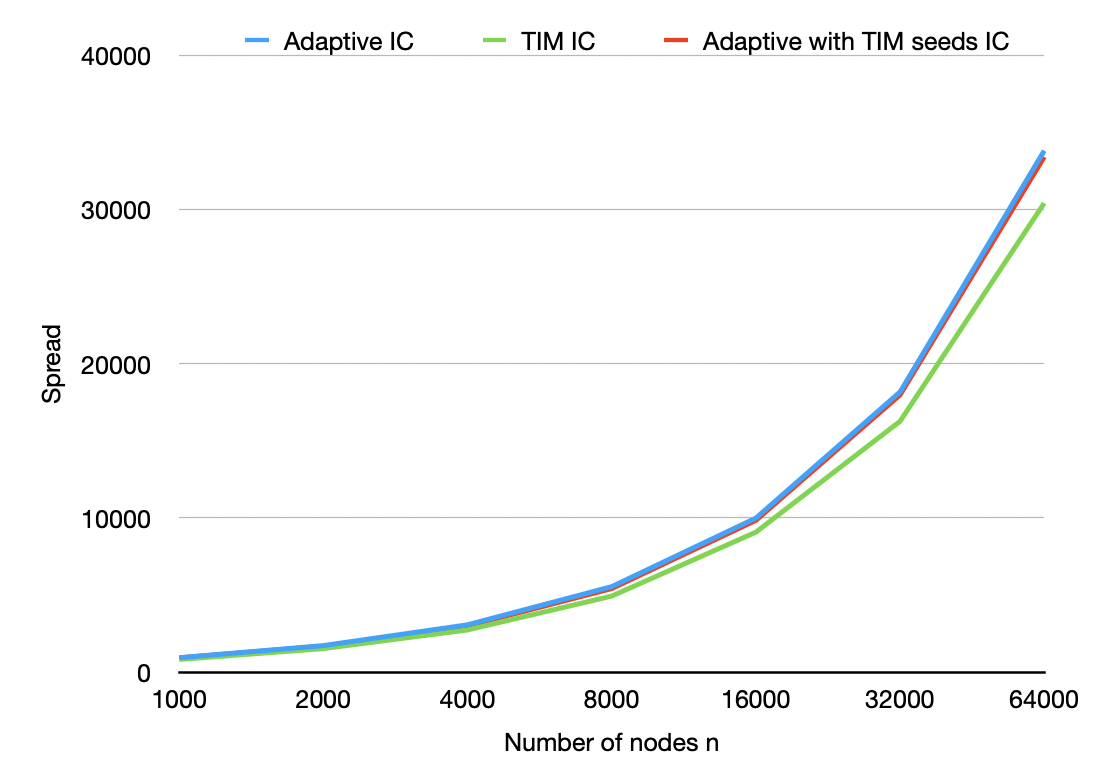
\includegraphics[width=1\linewidth]{GSSI_thesisProposal/figures/ER_IC.png}
    \caption{ER graph; $k=198$}
    \label{fig:first}
\end{subfigure}
\hfill
\begin{subfigure}{0.4\textwidth}
    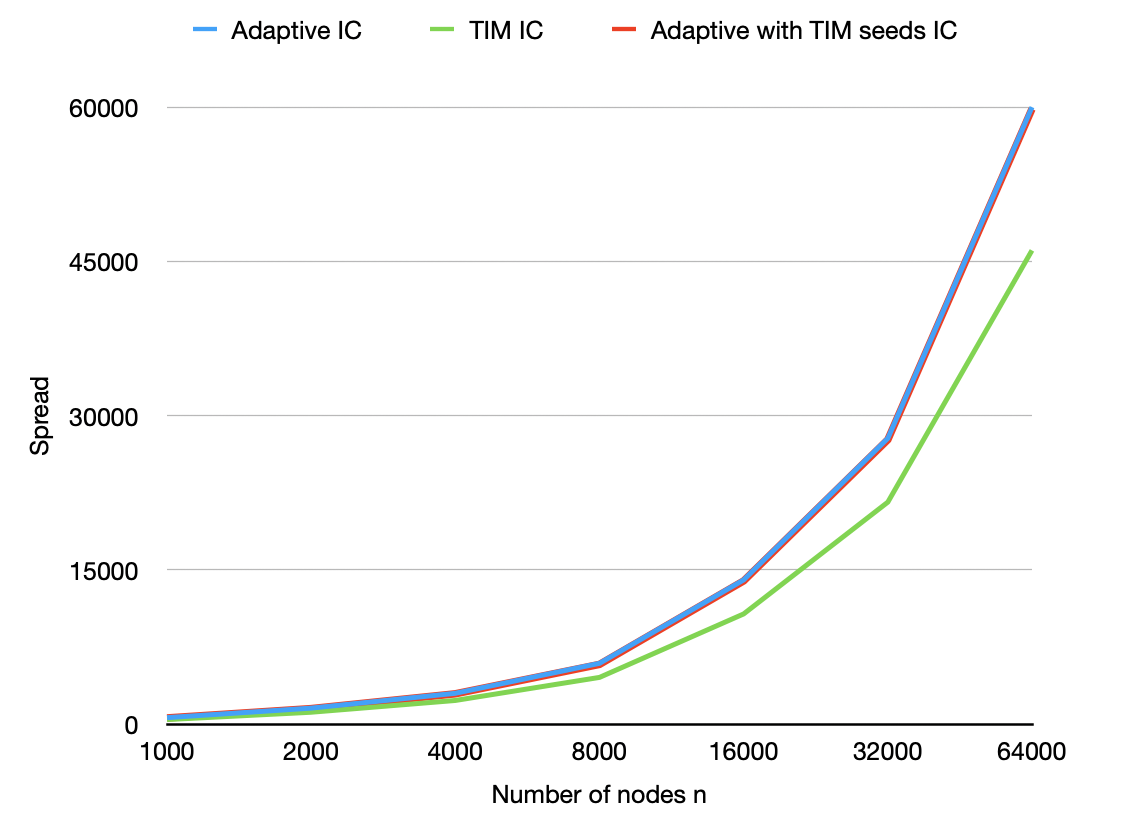
\includegraphics[width=1\linewidth]{GSSI_thesisProposal/figures/WS_IC.png}
    \caption{WS graph; $k=10$}
    \label{fig:second}
\end{subfigure}
\hfill
\begin{subfigure}{0.4\textwidth}
    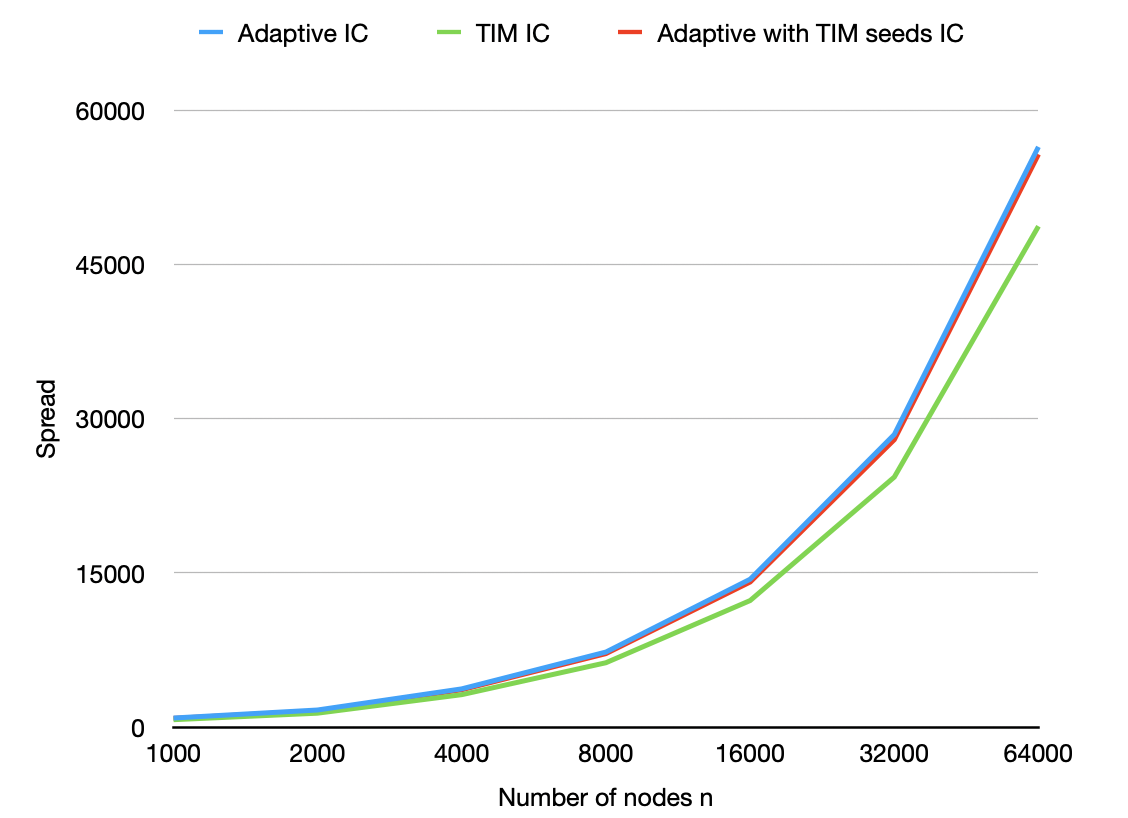
\includegraphics[width=1\linewidth]{GSSI_thesisProposal/figures/BA_IC.png}
    \caption{BA graph; $k=100$}
    \label{fig:third}
\end{subfigure}
\hfill
\begin{subfigure}{0.4\textwidth}
    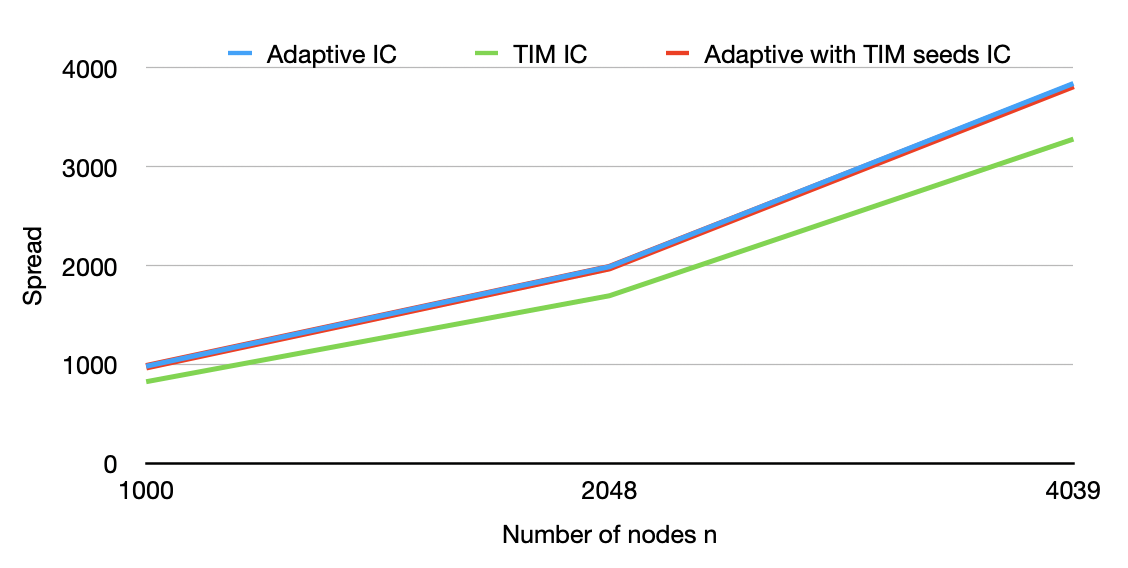
\includegraphics[width=1\linewidth]{GSSI_thesisProposal/figures/Fb_IC.png}
    \caption{Facebook network; $k=50$}
    \label{fig:fourth}
\end{subfigure}
        
\caption{Results under the Independent Cascade model with $p=[0.1,1.0]$.}
\label{fig:figure_IC}
\end{figure}


The figures in \ref{fig:figure_IC} represent the 4 different networks with the edge probability chosen at random between $[0.1,1.0]$. In general, the three generated graphs are comparable to each other with Barabasi-Albert having the best spread. From figure  \ref{fig:figure_IC} and table \ref{AG}, we observe that the seeds selected by the $TIM^+$ algorithm are nearly as good as the ones selected by the adaptive greedy TIM. For comparing the quality of selected seeds that the adaptive greedy TIM and $TIM^+$ produce, we introduce a new algorithm, called the adaptive greedy with TIM seeds, which take the seeds generated by $TIM^+$, but runs them on the same realisations generated by the adaptive greedy TIM. 


 \begin{table} [ht]
    \centering
    \begin{adjustbox}{width=1\textwidth}
    \begin{tabular}{ | c | c | c | c | }
    \hline
    \textit{Graph}& \textit{Greedy Adaptivity Gap}& \textit{Adaptive vs. greedy adaptive (TIM seeds)}& \textit{Greedy adaptive (TIM seeds) vs. $TIM+$}\\[2ex]
     \hline
    Erdős-Rényi& 1.2915& 1.00004& 1.2914\\ [2ex]
    Watts-Strogatz& 1.3024& 1.0031& 1.2983\\[2ex]
    Barabasi-Albert& 1.3155& 1.0068& 1.3067 \\[2ex]
    \hline
    \end{tabular}
    \end{adjustbox}
    \caption{Adaptive ratios with $n=64000$ and $k=10$ under the IC model for generated graphs.}
    \label{AG}
    \end{table}



    \begin{table} [ht]
    \centering
    \begin{adjustbox}{width=1\textwidth}
    \begin{tabular}{ | c | c | c | c | }
    \hline
    \textit{No.of nodes}& \textit{Greedy Adaptivity Gap}& \textit{Adaptive vs. greedy adaptive (TIM seeds)}& \textit{Greedy adaptive (TIM seeds) vs. $TIM+$}\\[2ex]
     \hline
    1000& 1.18872& 1.00497& 1.18285\\ [2ex]
    2048& 1.17294& 1.00458& 1.16759\\[2ex]
    4039& 1.17135& 1.00541& 1.16504\\[2ex]
    \hline
    \end{tabular}
    \end{adjustbox}
    \caption{Adaptive ratios for the Facebook network with $k=50$.}
    \label{FB}
    \end{table}

Table \ref{AG} represents the ratio of the synthetic networks with the three variants of the TIM algorithm, with the greedy adaptivity gap being the ratio between the adaptive greedy TIM and $TIM^+$. Table \ref{FB} shows the three sampled networks of the Facebook graph and their adaptive ratios of the spread, with $k=50$ generated via the TIM algorithms. The ratios are normally higher than $1$ because adaptive algorithms perform strictly better than the non-adaptive ones. The second column is the ratio between the adaptive greedy TIM and the adaptive greedy with the predetermined $TIM^+$ seeds. The ratios in this column tends to 1 which proves that the seeds selected by $TIM^+$ are capable of generating a spread close to its adaptive greedy equivalent. The third column is the column that is similar to the first one, where we compare the greedy adaptive with $TIM^+$ seeds and the $TIM^+$ algorithm. Notice that the values of this column is similar to the greedy adaptivity gap further proving that in this setting, $TIM^+$ seeds are almost as good as the seeds selected by the adaptive greedy policy.




We move on to Figure \ref{fig:figure_int} where we restrain the probability on edges between 0.1 and 0.2 to observe the spread obtained by the three algorithms. From the graph, we see that the seeds selected by $TIM^+$ has a coverage as good as the ones selected by the greedy adaptive policy for both, a synthetic ER graph and a real world Facebook network. We consider these two particular networks to show the difference in activation between a generated graph (ER has a low clustering coefficient which helps to understand the result for low activation probabilities), and the Facebook network represents a real world network. 



\begin{figure}
\centering
\begin{subfigure}{0.4\textwidth}
    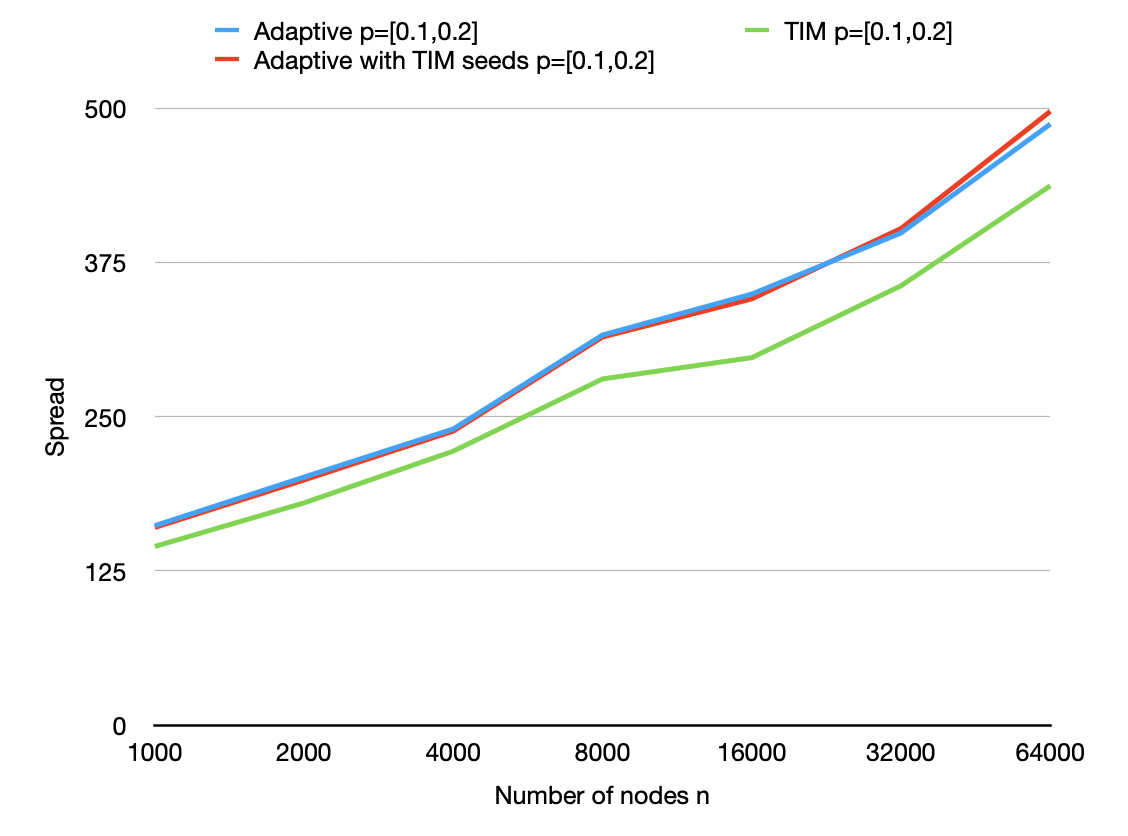
\includegraphics[width=1\linewidth]{GSSI_thesisProposal/figures/ER_int_IC.png}
    \caption{ER graph; $k=49$}
    \label{fig:first_int}
\end{subfigure}
\hfill
\begin{subfigure}{0.4\textwidth}
    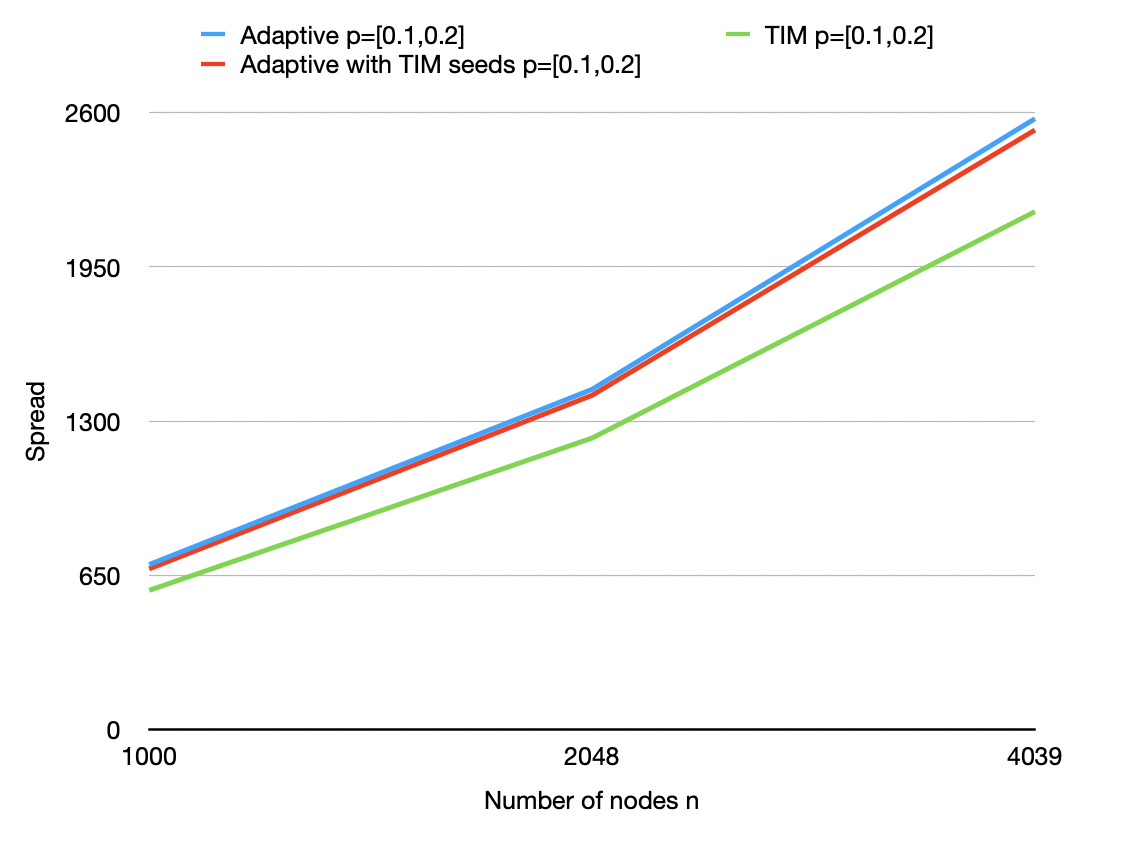
\includegraphics[width=1\linewidth]{GSSI_thesisProposal/figures/Fb_int_IC.png}
    \caption{Facebook network; $k=50$}
    \label{fig:second_int}
\end{subfigure}
\caption{Results under the Independent Cascade model with $p=[0.1,0.2]$.}
\label{fig:figure_int}
\end{figure}


%However, while running the programs, we used two different systems due to the overhead induced by the algorithms. While $TIM^+$ runs faster, the amount of memory required to generate around 200 seeds for a network of size 64000 nodes and 368160 edges (ER graph) is more or less equal to 50GB. Figure \ref{fig:tim_mem} shows the process being killed on a machine with 8GB RAM, when we try to find 30 seeds on a network of size 32000 nodes. Comparing that with figure \ref{fig:aim_mem}, observe that we can run two processes in parallel on a 8GB machine, when we are using the adaptive version of $TIM^+$. In terms of time, the adaptive algorithm with the same parameters took days to run, forcing us to add parallelism to the algorithm since the realisations are independent of each other. We could run three adaptive greedy algorithms in parallel on a machine with 8GB RAM, as shown in figure \ref{fig:aim_mem_er} for an ER graph with 32000 nodes, thus showing us that the adaptive greedy is memory efficient, unlike $TIM^+$.




In the end, since the results generated by the adaptive greedy TIM and $TIM^+$ almost converges, if we want a time efficient seed selection process, we will select $TIM^+$ but at a cost of huge memory overhead. On the other hand, if there is a constraint on the memory, and we need to use a personal computer to run huge networks, an adaptive greedy algorithm is what we want to use, but the time required to run such networks should be calculated in weeks, even when the realisations are run in parallel. 









\subsection{Linear Threshold}

Since the BA graph and the Facebook network have high clustering coefficients, we considered just the same ER and WS graphs we generated for observing the behaviour of LT w.r.t IC. Again, the values of $n$ range from 1000 to 64000. However, the generation of realisations for LT to run the adaptive greedy TIM differs from the IC. 

\paragraph{Parameters.}

The BA graph and most other real world networks are power-law networks, and we observed that the LT model doesn't perform well with these graphs under the adaptive setting. So we consider just ER and WS graphs for the LT. The parameters are the same as in independent cascade with the error parameter $\epsilon = 0.05$. The probability on edges is in between $[0.1,1.0]$ and $k=198$ for ER and $k=10$ for WS, since the WS graph has a high clustering coefficient, which helps in activating almost the entire network with a lesser $k$ value than that of ER. Separate realisations for adaptive TIM are generated according to the underlying LT diffusion model.

\paragraph{Results.}

From figure \ref{fig:second_LT} we immediately notice in the WS graph plot that the $TIM^+$ seeds do not perform as well as it was doing in the IC model. Table \ref{WS} compares the greedy adaptivity gap under both the diffusion models with the same parameters. We observe from the table that the greedy adaptivity gap on average increases by $\approx 65\%$ for the WS network under LT with 10 seeds.


The ER graph plot shows a slight convergence between the red and blue lines representing the spread of adaptive greedy and the adaptive greedy with $TIM^+$ seeds, but the seeds selected by $TIM^+$ still perform quite well when compared to that of WS. To understand why we notice such a deviation can be attributed to the fact that the adaptive greedy TIM is no longer submodular in the LT model, but the theory is not yet proven. The question remains, that experimentally, we see that both models with a high and low clustering coefficient performs better in the LT model as compared to its IC counter part, so is there a way to pass the submodularity requirement in order to reach better theoretical bounds on the adaptivity gap of the linear threshold model with the full-adoption feedback?   


  \begin{table} [ht]
    \centering
    \begin{adjustbox}{width=1\textwidth}
    \begin{tabular}{ | c | c | c | }
    \hline
    \textit{No.of nodes}& \textit{Greedy Adaptivity Gap (IC)}& \textit{Greedy Adaptivity Gap (LT)}\\[2ex]
     \hline
    1000& 1.41086& 2.45217\\ [2ex]
    2000& 1.34130& 3.37854\\[2ex]
    4000& 1.30168& 3.38854\\[2ex]
    8000& 1.30027& 3.51286\\[2ex]
    16000& 1.30840& 4.28206\\[2ex]
    32000& 1.28733& 4.45013\\[2ex]
    64000& 1.30238& 4.32444\\[2ex]
    \hline
    \end{tabular}
    \end{adjustbox}
    \caption{Greedy adaptivity gap for the WS network under IC and LT with $k=10$.}
    \label{WS}
    \end{table}



\begin{figure}
\centering
\begin{subfigure}{0.4\textwidth}
    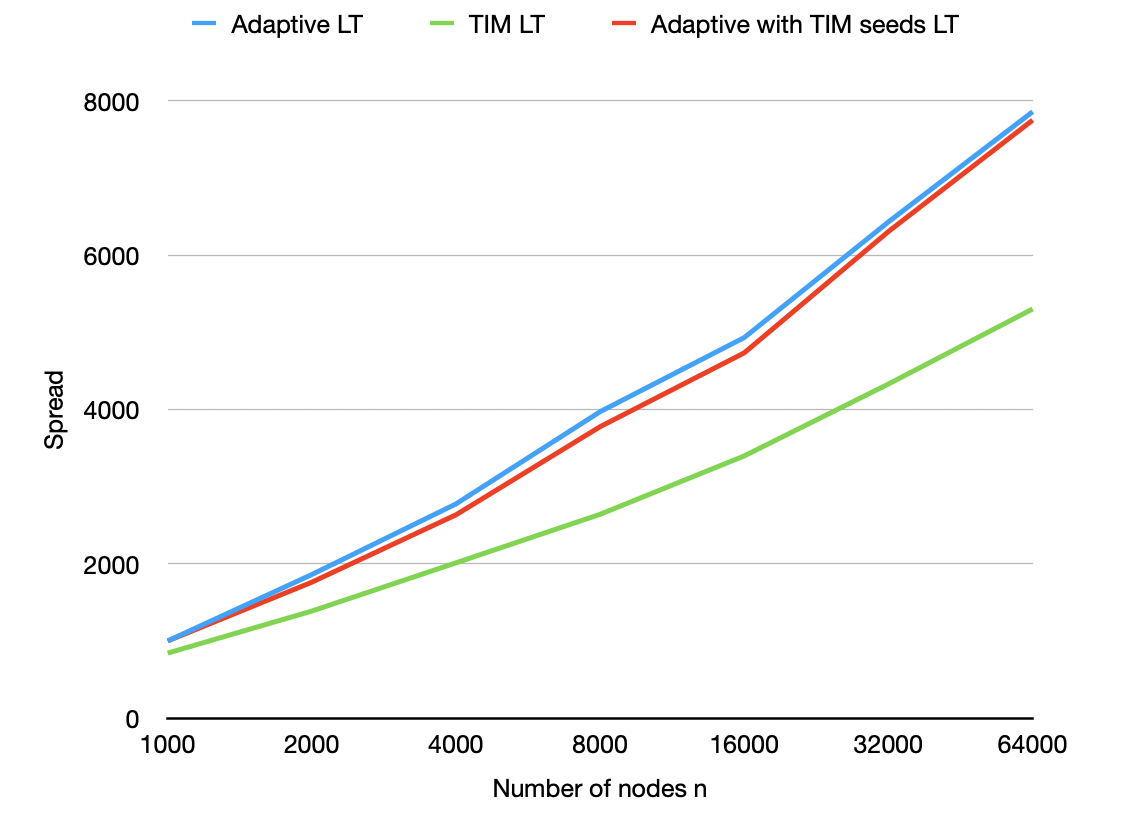
\includegraphics[width=1\linewidth]{GSSI_thesisProposal/figures/ER_LT.png}
    \caption{ER graph; $k=198$}
    \label{fig:first_LT}
\end{subfigure}
\hfill
\begin{subfigure}{0.4\textwidth}
    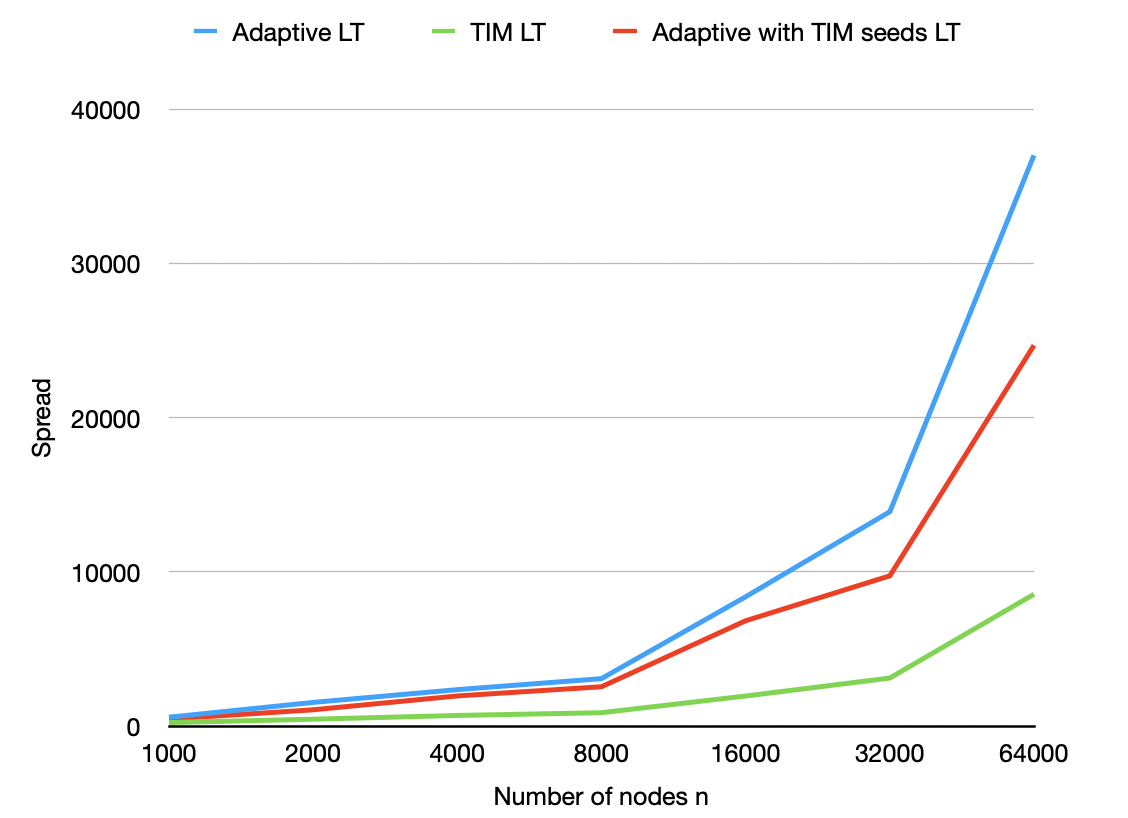
\includegraphics[width=1\linewidth]{GSSI_thesisProposal/figures/WS_LT.png}
    \caption{WS graph; $k=10$}
    \label{fig:second_LT}
\end{subfigure}
\caption{Results under the Linear Threshold model with $p=[0.1,1.0]$.}
\label{fig:figure_LT}
\end{figure}


\section{Summary}\label{sec_future_0}

This chapter studies the adaptivity gap of the independent cascade model with full-adoption feedback. We introduce a new technique to bridge the non-adaptive optimal and the adaptive optimal solution. Our technique directly builds the connection through defining the marginals related to the size $t-1$ non-optimal solution. 

First, we improve on the upper bound of the adaptivity gap for in-arborescences from $2e/(e-1)$ to $2e^2/(e^2-1)$. Second, we give an upper bound of $\lceil n^{1/3} \rceil$ for general graphs, which is the first sub-linear result on general graphs. Third, we show that for a class of $\alpha$-bounded graphs, the adaptivity gap is upper bounded by $\sqrt{\alpha}+O(1)$. Fourth, we prove that for a class of $(\beta,\gamma)$-bounded-activation graphs, we have an adaptivity gap of $\sqrt{\beta}+\frac{1}{1-\gamma}$. All the above results are based on our new technique.

We conduct some experiments on different type of synthetic and real world networks to understand the effect of adaptive greedy with the non-adaptive greedy algorithms. We give an overview of the greedy adaptivity gap to realize that even though the greedy adaptive algorithm is strictly better than the greedy non-adaptive policy, the adaptive greedy policy is not much better than the latter in both the IC and LT diffusion model. The adaptive greedy is memory efficient, whereas the non-adaptive greedy has a better efficiency in time. 
%----------------------------------------------------------------------------------------
%	ICALP
%----------------------------------------------------------------------------------------


\chapter{Improved Approximation Factor for Adaptive Influence Maximization via Simple greedy Strategies}\label{chap:sota}
\fancyhead[L]{\textit{Chapter 4. Improved Approximation via Greedy Strategies}}

In this chapter, we focus on the myopic model and analyze the approximation factor of the non-adaptive greedy algorithm without passing through the adaptivity gap [\ref{ag}]. We show that the algorithm achieves at least a fraction of $\frac{1}{2}\left(1-\frac{1}{e}\right)\approx 0.316$ of the adaptive optimum (Theorem \ref{thm1}). By definition, this implies that the adaptivity gap is at most $\frac{2e}{e-1}\approx 3.164$ (Remark \ref{adgapcor}). For both approximation ratio and adaptivity gap we obtain a substantial improvement with respect to the upper bounds obtained in \cite{Peng2019}, which are $\frac{1}{4}\left(1-\frac{1}{e}\right)\approx 0.158$ and $4$, respectively. 

Non-adaptive policies are strictly weaker than adaptive ones, since the latter can implement the former by simply ignoring any kind of feedback. On the other hand, adaptive policies are difficult to implement as they require to probe suitable seeds and to observe the corresponding feedback, which can be expensive and error-prone. Moreover, they may consist of exponentially-large decision trees that are hard to compute and store. In contrast, non-adaptive policies are easy to design and implement and are independent from the feedback. In particular, the non-adaptive greedy algorithm has been extensively studied and successfully applied in the field of influence maximization. For the non-adaptive setting, several efficient implementation of the greedy algorithm have been devised that allows us to use it in large real-world networks~\cite{Cohen14,Goyal11,Leskovec2007,Nguyen16,Tang15,Tang2014}. Our results show that the simple non-adaptive greedy algorithm performs well, even in the adaptive setting where we compare it with the adaptive optimum.

To show our bounds, we introduce a new approach that relate the non-adaptive greedy policy to an optimal adaptive solution. The new approach is not based on multilinear extensions and Poisson processes (like, e.g.~\cite{Asadpour16,Calinescu11,CVZ14,Chen2019}) neither on random walks on the optimal decision trees (like, e.g.~\cite{Bradac19,Gupta2016,Gupta2017,Peng2019}), which are the main tools used so far to relate adaptive and non-adaptive policies, and to bound the adaptivity gaps. Previous techniques derive adaptive approximation factors by combining non-adaptive approximation ratios with a bound on the adaptivity gap which is obtained by showing the existence of a ``good'' non-adaptive policy. However such a policy is hard to compute as it is usually  constructed by using an optimal adaptive policy. Our approach, instead, directly analyzes a non-adaptive policy and therefore provides the exact policy that gives the desired adaptivity gap and adaptive approximation factor. We believe that our approach is of independent interest and may be used to bound approximation factors and adaptivity gaps of different adaptive optimization problems. 

Our new approach consists in defining a simple randomized non-adaptive policy whose performance is not higher than that guaranteed by the greedy algorithm, and to relate such randomized non-adaptive policy with the optimal adaptive policy. In order to recover good properties of the objective function (like, e.g. submodularity) that usually guarantee good approximations when adopting  greedy strategies, we introduce an artificial diffusion process in which each seed has two chances to influence its neighbours. A similar process was introduced by Peng and Chen~\cite{Peng2019}, who consider a diffusion model in which the seeds appear in multiple copies of the influence graphs, so that, roughly speaking, each node has several chances to influence the neighbours, and the main machinery they consider to relate the optimal adaptive strategies with optimal non-adaptive ones are from Bradac et al.~\cite{Bradac19}.
Our direct and more refined analysis of the non-adaptive greedy algorithm improves, at the same time, both the approximation ratio and the adaptivity gap. 

To illustrate our approach, in Section~\ref{sec_example} we first apply our machinery to the simpler setting of adaptive monotone submodular maximization under cardinality constraint. As observed by Asadpour and Nazerzadeh~\cite{Asadpour16}, a constant factor approximation of the non-adaptive greedy policy applied to such setting can be obtained by combining the approximation ratio over the non-adaptive optimum and the adaptivity gap (which is equal to $\left(1-\frac{1}{e}\right)$~\cite{Asadpour16}); this leads to an approximation guarantee of $\left(1-\frac{1}{e}\right)^2\approx 0.399$. We give a more refined analysis of the non-adaptive greedy policy and show that its approximation ratio is at least $\frac{1}{2}\left(1-\frac{1}{e^2} \right)\approx 0.432$. Asadpour and Nazerzadeh \cite{Asadpour16} also showed that a so-called continuous greedy policy \cite{Calinescu11,CVZ14} achieves an approximation ratio of $1-\frac{1}{e}-\epsilon$ (in polynomial time w.r.t.~$\frac{1}{\epsilon}$). Since the continuous greedy policy is a non-adaptive policy, this bound is strictly better than ours. However, the non-adaptive greedy policy is simpler and deterministic, while the continuous greedy policy is randomized and more complex. 


Finally, in Section \ref{ad-sec}, we analyze the adaptive version of the greedy algorithm applied to the adaptive influence maximization problem. Again by resorting to an artificial diffusion process, we show that such adaptive algorithms guarantees an approximation ratio of $1-\frac{1}{\sqrt{e}} ~\approx~0.393$. Thus, we further improve the upper bound shown for the non-adaptive greedy algorithm, and we also give a more refined analysis of the adaptive greedy algorithm than that of Peng and Chen \cite{Peng2019}, who showed a $\frac{1}{4}\left(1-\frac{1}{e}\right)\approx 0.158$ approximation factor. 



\subsection*{Related Work.}
Golovin and Krause~\cite{Golovin2011a} conjectured that the influence maximization problem under the myopic feedback model admits a constant approximation algorithm and a constant adaptivity gap, despite the missing adaptive submodularity under such a feedback model. Since then, several studies have been conducted on the myopic feedback model. Some recent works include that of Salha et al.~\cite{Salha2018}, in which they consider a modified version of the independent cascade model which gives multiple chances to the seeds to activate their  neighbours, and  consider a different utility function which needs to be maximized. They demonstrate that the myopic feedback model is adaptive submodular under such modified diffusion model, and provide an adaptive greedy policy that achieves a $1-1/e$ approximation ratio for the problem of finding the best adaptive policy. The work of Peng and Chen~\cite{Peng2019} is the first to provide a constant upper bound on the adaptivity gap under the myopic feedback model. They introduce a policy in which each seed appears in multiple copies of the original graph; furthermore, this hybrid policy connects the adaptive and the non-adaptive policies via a  machinery used by \cite{Gupta2016,Gupta2017,Bradac19} in the context of stochastic probing. Peng and Chen~\cite{Peng2019} prove that the adaptivity gap lies in between $\left[e/(e-1),4\right]$, and by extension has a $(1-1/e)/4$ approximation factor. 

Singer et al.~\cite{Badanidiyuru2016,Rubinstein2015, Seeman2013, Singer2016}, in their line of research on adaptivity gaps, studied a two-stage process called adaptive seeding, that exhibits some similarities with the influence maximization problem under the myopic feedback model. Beyond influence maximization problems, adaptive optimization and adaptivity gaps has been generally studied for many other stochastic settings~\cite{DBLP:conf/stacs/AdamczykSW14,Asadpour16, DBLP:conf/wine/AsadpourNS08, Bradac19,DBLP:journals/mor/ChanF09,   DBLP:conf/soda/DeanGV05, DBLP:journals/mor/DeanGV08,DBLP:conf/latin/GoemansV06,   Golovin2011a,DBLP:conf/icml/GuilloryB10, Gupta2016,Gupta2017,DBLP:conf/ciac/HellersteinKL15,DBLP:journals/corr/abs-1803-07639,Bradac19}.

A general adaptive optimization framework deals with the fact that an item will reveal its actual state only when it has been irrevocably included in the final solution, and the main goal is to optimize an objective function under such uncertainty. Stochastic variants of packing integer programs, 0/1 knapsack, and covering problems, have been studied under the perspective of adaptive optimization in \cite{DBLP:conf/soda/DeanGV05, DBLP:journals/mor/DeanGV08,DBLP:conf/latin/GoemansV06}, respectively.

Asadpour et al.~\cite{Asadpour16, DBLP:conf/wine/AsadpourNS08} study the adaptivity gap of the stochastic submodular maximization problem under a matroid constraint, in which the goal is to select a subset of items satisfying a matroid constraint, that maximizes the value of a monotone submodular value function defined on the random states of the selected items. In~\cite{Asadpour16}, the authors consider an adaptive greedy policy (often denoted as the myopic policy) to approximate the optimal value of the best adaptive policy. They show that it achieves a $1/2$ approximation ratio under general matroid constraint, and a $1-\frac{1}{e}$ approximation ratio  under cardinality constraint. Interesting variants or extensions of the above optimization problem have been  considered in \cite{Bradac19,Gupta2016,Gupta2017}.

Chan and Farias~\cite{DBLP:journals/mor/ChanF09} study the efficiency of adaptive greedy policies applied to a general class of stochastic optimization problems, called stochastic depletion, in which the adaptive policy, at each step, chooses an action that generates a reward and depletes some of the items. They show that, under certain structural properties, a simple adaptive greedy policy guarantees a constant factor approximation of the best adaptive policy. Hellerstein et al.~\cite{DBLP:conf/ciac/HellersteinKL15} use an optimal decision tree to build a connection between the adaptive and the non-adaptive policies, and show that the adaptivity gap of stochastic submodular maximization under cardinality constraint is $1-\frac{1}{e^\tau}$, where $\tau$ is the minimum value of the probability that an  item is in some state. 

\subsection*{Contribution.}

The main contributions of this chapter lies in the new technique that we use to bound the approximation factor of the non-adaptive greedy algorithm, resulting in an improved bound of $\frac{1}{2}\left(1-\frac{1}{e}\right) \approx 0.316.$ The result is extended to also improve on the adaptivity gap to 3.164 from 4 for the myopic feedback under the independent cascade model. Finally, we also analyze the adaptive greedy algorithm, and show that it guarantees an improved approximation factor of  $1-\frac{1}{\sqrt{e}}\approx 0.393$.

\subsection*{Organization of the Chapter.}

In section Section~\ref{sec_example} we introduce our new approach by applying it to a simpler setting. We apply our technique to the stochastic submodular maximization problem and introduce the necessary notation and definitions. Section \ref{prel_myo} defines the AIM problem under the IC model with myopic feedback. In Section~\ref{sec_nag} we give the main results of this chapter, that is the improved approximation factor for the non-adaptive greedy algorithm and the upper bound on adaptivity gap for the adaptive influence maximization problem under myopic feedback. Finally, in Section~\ref{ad-sec} we show an improved approximation ratio for the adaptive greedy algorithm.  



\section{Stochastic Submodular Maximization} \label{sec_example}

In this section, we illustrate our machinery by applying part of it to the problem of maximizing a stochastic submodular set function under cardinality constraints~\cite{Asadpour16}. 

For two integers $h$ and $k$, $h\leq k$, let $[k]_h:=\{h,h+1,\ldots, k\}$ and $[k]:=[k]_1$. A function $f:\RP^n\rightarrow \RP$ is {\em a monotone submodular value function} if, for any vectors $x,y\in \RP$, we get $f(x\vee y)+f(x\wedge y)\leq f(x)+f(y)$, where $x\wedge y$ denotes the componentwise minimum and $x\vee y$ denotes the componentwise maximum.

Let $[n]$ be a finite set of $n$  items, and let $\bm \theta=(\bm \theta_1,\ldots, \bm \theta_n)$ be a vector of $n$ real, non-negative, and independent {\em state} random variables, where each $\bm \theta_i$ returns the state $\theta_i\in \RP$ associated to each item $i$ following a certain probability distribution. Let $f:\RP^n\rightarrow \RP$ be the {\em objective function}, that is a monotone submodular value function. For any $S\subseteq [n]$, let $\bm \theta(S):=(\bm \theta_1(S),\ldots, \bm \theta_n(S))$ be the {\em partial state} random variable, that is a random vector defined as $\bm \theta_i(S)=\bm \theta_i$ if $i\in S$, $\bm \theta_i(S)=0$ otherwise. With a little abuse of notation, we assume that vector $\bm \theta(S)$ gives also information on the set $S$ which $\bm \theta(S)$ is based on.

For a given integer $k\geq 0$, we aim at selecting a subset $S\subseteq [n]$ subject to cardinality constraint $|S|=k$, that maximizes the expected value $\E_{\bm \theta}[f(\bm \theta(S))]$. To guarantee a (possibly) better solution we can resort to an {\em adaptive policy}, that, at each step, observes the partial state $\xi\sim\bm \theta(U)$, where $U$ denotes the set of items previously selected, and selects another further item $\pi(\xi)\in [n]\setminus U$;  after $k$ iterations, the policy returns a set $U_{\bm\theta,k}(\pi)\subseteq [n]$ with $|U_{\bm\theta,k}(\pi)|=k$, which is a random set depending on the state of $\bm \theta$. The {\em stochastic monotone submodular maximization problem} (SMSM) takes as input a set of items $[n]$, a random vector~$\bm \theta$, a monotone submodular value function $f$, and an integer $k\in [n]$, and asks to find an adaptive policy $\pi$ that maximizes the expected value $\E_{\bm \theta}[f(\bm \theta(U_{\bm\theta,k}(\pi)))]$. 

In general, computing an optimal adaptive strategy is a computationally hard problem. Furthermore, in many contexts it is difficult to implement adaptive strategies, and non-adaptive strategies (in which the solution is chosen without observing the states of the random variables) is a more feasible choice. Asadpour and Nazerzadeh \cite{Asadpour16} show that a non-adaptive randomized continuous greedy algorithm guarantees a $\left(1-\frac{1}{e}-\epsilon\right)$ approximation for the SMSM problem (in polynomial time w.r.t. $1/\epsilon$); however, the proposed approach resorts to a quite sophisticated randomized algorithm. They also consider a simpler and deterministic {\em non-adaptive greedy algorithm} as approximation algorithm, that starts from an empty set $S:=\emptyset$ and, at each iteration $t\in [k]$, adds in $S$ the item $i\in [n]\setminus S$ maximizing $\E_{\bm \theta}[f(\bm \theta(S\cup\{i\}))]$. They show that the greedy algorithm guarantees an approximation factor of $\frac{1}{2}\left(1-\frac{1}{e}\right)\approx 0.316$ if the chosen subsets are subject to a matroid constraint, that can be reduced to $\left(1-\frac{1}{e}\right)^2\approx 0.399$ when considering a cardinality constraint $|S|\leq k$ only (i.e., uniform matroid constraint). 

In the following theorem, we give a better analysis of the greedy algorithm under cardinality constraints, and we show that the approximation factor increases to $\frac{1}{2}\left(1-\frac{1}{e^2}\right)\approx 0.432$. 

\begin{theorem}\label{thm0}
The non-adaptive greedy algorithm is a $\frac{1}{2}\left(1-\frac{1}{e^2}\right)$ approximation algorithm for the SMSM problem. 
\end{theorem}
For the proof of Theorem \ref{thm0} we relate the non-adaptive greedy solution with the optimal adaptive solution. We assume w.l.o.g that $k\geq 2$, otherwise the approximation ratio is equal to~$1$. For any $t\in [k]_0$, let $S_t$ be the set of $t$ items computed by the greedy algorithm at iteration $t$ (where $S_0:=\emptyset$). Let $ \pi$ be an optimal adaptive policy, and let $x=(x_1,\ldots, x_n)\in [0,1]^n$ be the vector such that $x_i$ is the probability that node $i\in [n]$ is selected by policy $\pi$. Let $OPT_A(k)$ denote the value of policy $\pi$ (i.e., the optimal value of the problem). Given $i\in [n]$, let $\bm e^{i}:=(\bm e^{i}_1,\ldots, \bm e^{i}_n)$ be a random vector where $\bm e^{i}_j$ has the same distribution of $\bm\theta_i$ if $i=j$, and $\bm e^{i}_j=0$ otherwise; given a partial state $\xi$, let $\Delta(i|\xi):=\E_{\bm e^i}[f(\xi \vee \bm e^{i})-f(\xi)],$ i.e., the expected increment of the objective function when adding an item $i$ under partial state $\xi$.

For any $t\in [k-1]_0$, as intermediate step of our analysis, we consider a {\em randomized non-adaptive policy} ${\sf Rand}_t$ that, starting from the greedy solution $S_{t}$, computes a random set $S_{\bm\rho,t}:=S_{t}\cup\{\bm \rho\}$, where $\bm\rho\in [n]$ is a random item such that $\mathbb{P}[\bm\rho=i]=x_i/k$ for any $i\in [n]$ and selected independently from any other event. Observe that the above random variable is well-defined, as $\sum_{v\in V}(x_v/k)=k/k=1$; furthermore, we observe that the expected value of $f$ under ${\sf Rand}_{t}$ is $\E_{\bm\theta,\bm\rho}[f(\bm \theta(S_{\bm\rho,t})]$. Furthermore, for any $t\in [k-1]_0$, we consider a {\em hybrid adaptive policy} ${\sf Hyb}_{t}$, that first runs the adaptive policy $\pi$, and then merges the items of $S_t$ with the items of $U_{\hat{\bm\theta},k}(\pi)$ selected by $\pi$, where $\hat{\bm \theta}$ is a random state that follows the same distribution of $\bm \theta$ but is  independent from $\bm \theta$; finally, the expected value of $f$ under ${\sf Hyb}_{t}$ is defined as $\E_{\bm\theta,\hat{\bm \theta}}[f(\bm\theta(S_t)\vee\hat{\bm \theta}(U_{\hat{\bm\theta},k}(\pi)\cup S_t))].$

A similar hybrid adaptive policy has been also considered by Asadpour and Nazerzadeh \cite{Asadpour16}, but in place of the randomized non-adaptive policy considered in our work, they resort to a non-adaptive strategy defined by a Poisson process based on the multilinear extension of the expected value function $\E_{\bm \theta}[f(*)]$. Before showing the theorem, we give some preliminary lemmas, which relate the randomized non-adaptive policy with the hybrid adaptive policy.

\begin{lemma}\label{lemprel1}
We have that $\E_{\bm \theta,\bm \rho}[f(\bm\theta(S\cup\{\bm \rho\}))]-\E_{\bm \theta}[f(\bm\theta(S))]= \sum_{i\in [n]\setminus S}x_i\cdot \E_{\bm\theta}[\Delta(i|\bm\theta(S))]$ for any $S\subseteq [n]$.
\end{lemma}
\begin{proof}
As $\mathbb{P}[\bm \rho=i]=\frac{x_i}{k}$ for any $i\in [n]$, we have that 
\begin{align*}
&\E_{\bm \theta,\bm \rho}[f(\bm\theta(S\cup\{\bm \rho\}))]-\E_{\bm \theta}[f(\bm\theta(S))]\\
&=k\cdot \E_{\bm \rho}[\E_{\bm\theta}[f(\bm\theta(S\cup{\bm \rho}))-f(\bm\theta(S))]]\\
&=k\cdot \sum_{i\in [n]\setminus S} \mathbb{P}[{\bm \rho}=i]\cdot \E_{\bm\theta}[\Delta(i|\bm\theta(S))]\\
&=k\cdot \sum_{i\in [n]\setminus S} \frac{x_i}{k}\cdot \E_{\bm\theta}[\Delta(i|\bm\theta(S))]\\
&=\sum_{i\in [n]\setminus S} x_i\cdot \E_{\bm\theta}[\Delta(i|\bm\theta(S))].
\end{align*}
\end{proof}


\begin{lemma}\label{lemprel2}
For any $S\subseteq [n]$, we have $\E_{\bm\theta,\hat{\bm \theta}}[f(\bm\theta(S)\vee\hat{\bm \theta}(U_{\hat{\bm\theta},k}(\pi)\cup S))]\\
\leq \E_{\bm\theta,\hat{\bm \theta}}[f( \bm\theta(S)~\vee~\hat{\bm \theta}(S)]+\sum_{i\in [n]\setminus S}x_i\cdot \E_{\bm\theta}[\Delta(i|\bm\theta(S))]$.
\end{lemma}

\begin{proof}
It is sufficient to show that $\E_{\hat{\bm \theta}}[f(\xi\vee\hat{\bm \theta}(U_{\hat{\bm\theta},k}(\pi)\cup S))]\leq \E_{\hat{\bm \theta}}[f(\xi\vee\hat{\bm \theta}(S)]+\sum_{i\in [n]\setminus S}x_i\cdot \Delta(i|\xi)$ for any partial state $\xi\sim \bm\theta(S)$, so that, by doing the expectation on $\xi\sim\bm\theta(S)$, the claim follows. 

We observe that $\E_{\hat{\bm \theta}}[f(\xi\vee\hat{\bm \theta}(U_{\hat{\bm\theta},k}(\pi)\cup S))]$ can be rewritten as the expected value $\E_{\hat{\bm \theta}}[f(\xi\vee\hat{\bm \theta}(S))]$ coming from the selection of $S$, plus the sum of expected increments of $f$ caused by all the nodes $i\in [n]\setminus S$ selected by policy $\pi$, when observing partial states from $\hat{\bm \theta}$. We have that the second sum can be written as  $$\sum_{i\in [n]\setminus S}\sum_{\hat{\xi}}\chi(i|\hat{\xi})\cdot \Delta(i|\xi\vee \hat{\xi}),$$ where $\chi(i|\hat{\xi})\in \{0,1\}$ is the indicator random variable that is equal to $1$ if policy $\pi$ visits state $\hat{\xi}$ at some step of the execution and then selects node $i$ (i.e., $i=\pi(\hat{\xi})$), and $\chi(i|\hat{\xi})=0$ otherwise. Thus,
\begin{align}
&\E_{\hat{\bm \theta}}[f(\xi\vee\hat{\bm \theta}(U_{\hat{\bm\theta},k}(\pi)\cup S))]\nonumber\\
&=\E_{\hat{\bm \theta}}[f(\xi\vee\hat{\bm \theta}(S))]+\sum_{i\in [n]\setminus S}\sum_{\hat{\xi}}\chi(i|\hat{\xi})\cdot \Delta(i|\xi\vee \hat{\xi}).\label{xi1}
\end{align}
For any partial state $\hat{\xi}$ we have that
\begin{align}
&\Delta(i|\xi\vee \hat{\xi})]\nonumber\\
&=\E_{\bm e^i}[f(\xi \vee \hat{\xi}\vee \bm e^{i})-f(\xi\vee \hat{\xi})]\nonumber\\
&=\E_{\bm e^i}[f((\xi \vee \hat{\xi})\vee (\xi\vee \bm e^{i}))-f(\xi\vee \hat{\xi})]\nonumber\\
&\leq \E_{\bm e^i}[f(\xi \vee \bm e^{i})-f((\xi\vee \hat{\xi})\wedge (\xi\vee \bm e^{i}))]\label{xi1.1}\\
&\leq  \E_{\bm e^i}[f(\xi \vee \bm e^{i})-f(\xi)]\nonumber\\
&=\Delta(i|\xi),\label{xi2}
\end{align}
where \eqref{xi1.1} holds since $f$ is a monotone submodular value function: indeed, we have that $f(x\vee y)+f(x\wedge y)\leq f(x)+f(y)$ with $x:=(\xi \vee \hat{\xi})$ and $y:= (\xi\vee \bm e^{i})$, thus showing \eqref{xi1.1}. Furthermore, by exploiting the fact that $x_i$ is the probability that an item $i$ is selected in some step of policy $\pi$, we get
\begin{equation}\label{xi3}
\sum_{\hat{\xi}}\chi(i|\hat{\xi})=x_i.
\end{equation}
Finally, by combining \eqref{xi1}, \eqref{xi2}, and \eqref{xi3}, we get
\begin{align*}
&\E_{\hat{\bm \theta}}[f(\xi\vee\hat{\bm \theta}(U_{\hat{\bm\theta},k}(\pi)\cup S))]\\
&=\E_{\hat{\bm \theta}}[f(\xi\vee\hat{\bm \theta}(S))]+\sum_{i\in [n]\setminus S}\sum_{\hat{\xi}}\chi(i|\hat{\xi})\cdot \Delta(i|\xi\vee \hat{\xi})\\
&\leq \E_{\hat{\bm \theta}}[f(\xi\vee\hat{\bm \theta}(S))]+\sum_{i\in [n]\setminus S}\sum_{\hat{\xi}}\chi(i|\hat{\xi})\cdot \Delta(i|\xi)\\
&=\E_{\hat{\bm \theta}}[f(\xi\vee\hat{\bm \theta}(S))]+\sum_{i\in [n]\setminus S}\left(\sum_{\hat{\xi}}\chi(i|\hat{\xi})\right)\cdot \Delta(i|\xi)\\
&=\E_{\hat{\bm \theta}}[f(\xi\vee\hat{\bm \theta}(S))]+\sum_{i\in [n]\setminus S}x_i\cdot \Delta(i|\xi),
\end{align*}
thus showing the claim. 
\end{proof}

\begin{lemma}\label{lemprel3}
We have that $OPT_A(k)\leq \E_{\bm\theta,\hat{\bm \theta}}[f(\bm\theta(S)\vee \hat{\bm \theta}(U_{\hat{\bm\theta},k}(\pi)\cup S))]$ for any $S\subseteq [n]$.
\end{lemma}

\begin{proof}
The claim easily follows from the fact that $\hat{\bm \theta}(U_{\hat{\bm\theta},k}(\pi))$ is componentwise non-higher than $\bm\theta(S)\vee \hat{\bm \theta}(U_{\hat{\bm\theta},k}(\pi)\cup S)$, thus, as $f$ is monotone we get $OPT_A(k)=\E_{\hat{\bm \theta}}[f(\hat{\bm \theta}(U_{\hat{\bm\theta},k}(\pi)))]\leq \E_{\bm\theta, \hat{\bm \theta}}[f(\bm\theta(S)\vee \hat{\bm \theta}(U_{\hat{\bm\theta},k}(\pi)\cup S))].$ 
\end{proof}

Armed with the above lemmas, we can prove Theorem \ref{thm0}.
\begin{proof}[Proof of Theorem \ref{thm0}]
For any $t\in [k]_0$, let $GR_N(t):=\E_{\bm \theta}[f(\bm \theta(S_t))]$ denote the expected value of $f$ obtained at the $t$-th iteration of the non-adaptive greedy algorithm. We have that
\begin{align}
&GR_N(t+1)-GR_N(t)=\max_{v\in V}\left[\E_{\bm \theta}[f(\bm\theta(\{v\}\cup S_t))]\right]-\E_{\bm \theta}[f(\bm\theta(S_t))]\label{equ0prel}\\
&\geq \overbrace{\E_{\bm \theta,\bm \rho}[f(\bm\theta(S_{t}\cup\{\bm \rho\}))]}^{\text{Exp. value of }{\sf Rand}_t}-\E_{\bm \theta}[f(\bm\theta(S_t))]\nonumber\\
&\geq \frac{1}{k}\cdot \sum_{i\in [n]\setminus S_t}x_i\cdot \E_{\bm\theta}[\Delta(i|\bm\theta(S_t))]\label{equ1prel}\\
&\geq \frac{1}{k}\cdot\left(\overbrace{\E_{\bm\theta,\hat{\bm \theta}}[f(\bm\theta(S_t)\vee \hat{\bm \theta}(U_{\hat{\bm\theta},k}(\pi)\cup S_t))]}^{\text{Exp. value of }{\sf Hyb}_t}-\E_{\bm\theta,\hat{\bm \theta}}[f( \bm\theta(S_t)\vee\hat{\bm \theta}(S_t))]\right)\label{equ2prel}\\
&\geq \frac{1}{k}\cdot\left(OPT_A(k)-\E_{\bm\theta,\hat{\bm \theta}}[f( \bm\theta(S_t)\vee\hat{\bm \theta}(S_t))]\right)\label{equ3prel}\\
&\geq \frac{1}{k}\cdot OPT_A(k)-\frac{1}{k}\cdot \left(\E_{\bm\theta,\hat{\bm \theta}}[f( \bm\theta(S_t))+f( \hat{\bm\theta}(S_t))]\right)\label{equ4prel}\\ 
&\geq \frac{1}{k}\cdot OPT_A(k)-\frac{1}{k}\cdot \left(\E_{\bm\theta}[f( \bm\theta(S_t))]+\E_{\hat{\bm \theta}}[f( \hat{\bm\theta}(S_t))]\right)\nonumber\\
&= \frac{1}{k}\cdot OPT_A(k)
-\frac{2}{k}\cdot \E_{\bm\theta}[f(\bm\theta(S_t)]\nonumber\\
&=\frac{1}{k}\cdot OPT_A(k)-\frac{2}{k}\cdot GR_N(t),\label{equfundprel}
\end{align}
where \eqref{equ0prel} comes from the fact that the greedy strategy, at iteration $t+1$, adds to $S_t$ the item $i$ guaranteeing the best expected value of $f$, \eqref{equ1prel} comes from Lemma \ref{lemprel1}, \eqref{equ2prel} comes from Lemma \ref{lemprel2}, \eqref{equ3prel} comes from Lemma \ref{lemprel3}, and \eqref{equ4prel} holds since $f$ is a monotone submodular value function (as $f(\bm\theta(S_t)\vee\hat{\bm \theta}(S_t))\leq f(\bm\theta(S_t)\vee\hat{\bm \theta}(S_t))+f(\bm\theta(S_t)\wedge\hat{\bm \theta}(S_t))\leq f( \bm\theta(S_t))+f( \hat{\bm\theta}(S_t))$). Thus, by \eqref{equfundprel} and some manipulations, we get $
{GR}_N(t+1)\geq \frac{1}{k}\cdot OPT_A(k)+\left(1-\frac{2}{k}\right)\cdot {GR}_N(t)$ for any $t\in [k-1]_0.$ By applying iteratively the above inequality, we get $
{GR}_N(k)\geq \frac{1}{k}\cdot \sum_{t=0}^{k-1}\left(1-\frac{2}{k}\right)^{t}\cdot OPT_A(k)=\frac{1}{2}\left(1-\left(1-\frac{2}{k}\right)^{k}\right)\cdot OPT_A(k),$ that leads to $\frac{{GR}_N(k)}{OPT_A(k)}\geq \frac{1}{2}\left(1-\left(1-\frac{2}{k}\right)^{k}\right) \geq \frac{1}{2}\left(1-\frac{1}{e^2}\right),$ and this shows the claim. 
\end{proof}


\section{Adaptive Influence Maximization under the Myopic Feedback Model: Preliminaries}\label{prel_myo}


\subparagraph*{Non-adaptive Influence Maximization.} Defined in Chapter \ref{chap:background}. Refer to Chapter \ref{chap:lit}, Sections \ref{main}--\ref{nonada_sec} for a more detailed overview. 


\subparagraph*{Adaptive Influence Maximization.} Differently from the non-adaptive setting, in which all the seeds are selected at the beginning, an {\em adaptive policy} activates the seeds sequentially in $k$ steps,
one seed at each step, and the decision on the next seed to select is based on the feedback resulting from the observed spread of previously selected nodes. The feedback model considered in this work is {\em myopic}: when a node is selected, the adaptive policy observes the state of its neighbours. 

An adaptive policy under the myopic feedback model is formally defined as follows. Given $L\subseteq E$, the {\em realisation} $\phi_L:V\rightarrow 2^V$ associated to $L$ assigns to each node $v\in V$ the value $\{z\in V:(v,z)\in L\}\cup\{v\}$, i.e., the set containing $v$ and the neighbours activated by seed $v$ when $\bm L=L$. Let $\Phi$ denote the {\em random realisation}, i.e., the random variable such that $\mathbb{P}[\Phi=\phi_L]=\mathbb{P}[\bm L=L]$ for any $L\subseteq E$. Given a set $S\subseteq V$, a {\em partial realisation} $\psi:S\rightarrow 2^V$ is the restriction to $S$ of the domain of some realisation, i.e., there exists $L\subseteq E$ such that $\psi(v)=\phi_L(v)$ for any $v\in S$. Given a partial realisation $\psi:S\rightarrow 2^V$, let $dom(\psi):=S$, i.e., $dom(\psi)$ is the domain of partial realisation $\psi$, and let $Im(\psi):=\bigcup_{v\in dom(\psi)}\psi(v)$. A~partial realisation $\psi'$ is a {\em sub-realisation} of a partial realisation $\psi$ (or, equivalently,  $\psi'\subseteq \psi$), if $dom(\psi')\subseteq dom(\psi)$ and $\psi'(v)=\psi(v)$ for any $v\in dom(\psi')$. We observe that any partial realisation $\psi$ can be equivalently represented as $\{(v,\phi_L(v)):v\in dom(\psi)\}$ for some $L\subseteq E$. 


An adaptive policy $\pi$ takes as input a partial realisation $\psi$ and, either returns a node $\pi(\psi)\in V$ and activates it as seed, or interrupts the activation of new seeds, e.g., by returning a string $\pi(\psi):=STOP$. In particular, an adaptive policy $\pi$ can be run as follows: (i) start from an empty realisation $\psi:=\emptyset$; (ii) if $\pi(\psi)\neq STOP$ set $\psi\leftarrow \psi\cup \{(v,\phi_L(v))\}$ and repeat (ii) until $\pi(\psi)=STOP$; (iii) at the end,  return $\psi_{\pi}:=\psi$. Let $\Psi_{\pi}$ be the random partial realisation returned by the execution of policy $\pi$. The {\em expected influence spread} of an adaptive policy $\pi$ is defined as $\sigma(\pi):=\mathbb{E}_{\bm L}[\sigma_{\bm L}(dom(\Psi_{\pi}))]$, i.e., it is the expected value of the number of nodes reached by the diffusion process at the end of the execution of policy $\pi$. We say that $|\pi|=k$ if policy $\pi$ always return a partial realisation $\psi_{\pi}$ with $|dom(\psi_{\pi})|=k$. The {\em adaptive influence maximization problem (under IC and myopic feedback)} is the computational problem that, given an influence graph $G$ and $k\in [n]$, asks to find an adaptive policy $\pi$ subject to $|\pi|=k$ that maximizes the expected influence spread $\sigma(\pi)$. 

The adaptive influence maximization defined above is analogous to the definition in chapter \ref{chap:background} section \ref{sec_prel}, however, we need new notations to cope with the new proof arguments for the myopic feedback. We redefine the AIM scenario again in this chapter for the sake of clarity and completeness.

\subparagraph*{Adaptivity Gap.} Defined formally in Section \ref{ag} Chapter \ref{chap:background}.


\section{Efficiency of Non-Adaptive Greedy algorithm} \label{sec_nag}
In this section, we show that a simple non-adaptive algorithm guarantees an approximation ratio of $\frac{1}{2}\left(1-\frac{1}{e}\right)\approx 0.316$ for the adaptive influence maximization problem, thus improving the approximation ratio of $\frac{1}{4}\left(1-\frac{1}{e}\right)\approx 0.158$ given in~\cite{Peng2019}. The algorithm provided by~\cite{Peng2019} is the usual {\em non-adaptive greedy algorithm} given in~\cite{Kempe2015} and reported in the previous section.

We observe that such algorithm is non-adaptive, i.e., despite it is used for adaptive optimization, does not resort to the use of any adaptive policy and all the seeds are selected without observing any partial realisation. 
\begin{theorem}\label{thm1}
Given an influence graph $G$ with $n$ nodes and $k\in [n]_2$, the non-adaptive greedy algorithm is a $\frac{1}{2}\left(1-\left(1-\frac{1}{k}\right)^{k}\right)\geq \frac{1}{2}\left(1-\frac{1}{e}\right)$ approximation algorithm for the adaptive influence maximization problem (under IC and myopic feedback) applied to $(G,k)$. 
\end{theorem}
In the proof of Theorem~\ref{thm1} (see Subsection \ref{proofthm1}) we relate the expected influence spread coming from the non-adaptive greedy algorithm with that of the optimal adaptive policy. We first need some notation and preliminary results. Let $G=(V=[n],E,(p_{uv})_{(u,v)\in E})$ be an influence graph, and let $k\in [n]_2$. For any $t\in [k]_0$, let $S_t$ denote the set of the first $t$ seeds selected by the greedy algorithm, so that $\sigma(S_k)$ is the expected influence spread of the solution returned by the algorithm. Let $\pi$ be an optimal adaptive policy, and let $x=(x_1,\ldots, x_n)$ be the vector such that $x_i$ is the probability that node $i$ is selected by $\pi$. As in Section~\ref{sec_example}, we resort again to a randomized non-adaptive policy to relate the expected influence spread of the greedy algorithm with that of the adaptive policy.

\subparagraph*{Randomized Non-adaptive Policy.} For any $t\in [k-1]_0$, as intermediate step of our analysis, we consider again the randomized non-adaptive policy ${\sf Rand}_t$ defined in Section~\ref{sec_example}: starting from the greedy solution $S_{t}$, we compute a random set $S_{\bm\rho,t}:=S_{t}\cup\{\bm \rho\}$, where $\bm\rho\in [n]$ is a random item such that $\mathbb{P}[\bm\rho=i]=x_i/k$ for any $i\in [n]$ and selected independently from any other event. We observe that the expected value of $f$ under ${\sf Rand}_{t}$ is $\E_{\bm \rho}[\sigma(S_{\bm\rho,t})]$. 

As a support of our analysis, we also define a new diffusion model and a hybrid adaptive policy. In particular, the new diffusion model will be used to recover certain properties connected with the submodularity that, as in Section~\ref{sec_example}, will allow us to relate the expected influence spread of the randomized non-adaptive policy with that of the hybrid adaptive policy. Furthermore, following again the approach of Section \ref{sec_example}, the hybrid adaptive policy is obtained by combining the greedy (non-adaptive) solution and the optimal adaptive one, and it will be used in our analysis to get an upper bound on the optimal adaptive spread. 



\subparagraph*{2-level Diffusion Model.} In the 2-level diffusion model each selected seed $u\in V$ has two chances to influence its neighbours, and all the non-seeds have one chance only, i.e., the activation probability for all the edges $(u,v)$ is $1-(1-p_{u,v})^2$ if $u$ is a seed, and $p_{u,v}$ otherwise. More formally, let $ \hat{\bm L}$ be a live-edge graph distributed as $\bm L$ and independent from $\bm L$. Given a set of seeds $S$, the {\em 2-level live-edge graph} can be defined as $\bm L^2(S):=\bm L\cup \{\hat{\bm L}\cap \{(u,v)\in E:u\in S\}\}$. Given a set of nodes $S$, let $\sigma^2_{\bm L,\hat{\bm L}}(S):=\sigma_{\bm L^2(S)}(S)$ denote the influence spread induced by $S$ in live-edge graph $\bm L^2(S)$, and let $\sigma^2(S):=\mathbb{E}_{\bm L,\hat{\bm L}}[\sigma^2_{\bm L,\hat{\bm L}}(S)]$ denote the expected influence spread induced by $S$ under the $2$-level diffusion model. Let $ \Phi$ and $\hat{\Phi}$ denote the random realisations associated to live-edge graphs $\bm L$ and $\hat{\bm L}$, respectively.

\subparagraph*{2-Level Hybrid Adaptive Policy.}  For any $t\in [k-1]_0$, let ${\sf Hyb}^2_{t}$ be a hybrid adaptive policy defined as follows: (i) ${\sf Hyb}^2_{t}$ selects all the nodes in $S_t$ as seeds; (ii) then, ${\sf Hyb}^2_{t}$ adds to $S_t$ all the nodes that the optimal adaptive policy $\pi$ would have select when starting from the empty realisation, and observing, at each step, partial realisations coming from the live-edge graph $\hat{\bm L}$ only; in other words, for any seed $v\in V$ selected by the policy, the new set of nodes that the policy observes (to choose the next seed) is $\hat{\Phi}(v)$; (iii) finally, denoting with $\hat{\Psi}_{\pi}$ the random realisation returned by $\pi$, the expected influence spread of ${\sf Hyb}^2_{t}$ is defined as $\E_{\bm L,\hat{\bm L}}[\sigma^2_{\bm L,\hat{\bm L}}(dom(\hat{\Psi}_{\pi})\cup S_t)]$, i.e., it is the expected influence spread determined $dom(\hat{\Psi}_{\pi})\cup S_t$, according to the 2-level live-edge graph $\bm L^2(dom(\hat{\Psi}_{\pi})\cup S_t)$.

In what follows we give some technical results which are based on the above definitions and will be used in Subsection \ref{proofthm1} to show the main theorem. In particular, we show that the 2-level diffusion model satisfies certain properties connected with submodular set functions (see Subsection \ref{sub1}); then, we use such properties to relate the expected influence spread in the ordinary diffusion model to that of the 2-level diffusion model (see Subsection \ref{sub2}); finally, by using a similar approach as in Section \ref{sec_example}, we use the above relations to relate the efficiency of the randomized non-adaptive policy with that of the optimal adaptive policy, via the 2-level hybrid adaptive policy (see Subsection \ref{sub3}). 

\subsection{Adaptive Submodularity in the 2-Level Diffusion Model}\label{sub1} The adaptive submodularity \cite{Golovin2011a} is a property that extends  the well-known concept of submodularity to the adaptive framework, and allows us to design efficient adaptive approximation algorithms. In particular, the adaptive submodularity states that, given two subrealisations $\psi\subseteq \psi'$ and a node $v\in V$, adding node $v$ under partial realisation $\psi'$ causes an expected increment of the influence spread that is not higher than that caused under partial realisation $\psi$. Unfortunately, as shown in  the arXiv version of \cite{Golovin2011a}, the myopic feedback model, in general, does not satisfy the adaptive submodularity. 

Anyway, by resorting to the 2-level diffusion model, we can recover a similar property as the adaptive submodularity. Given $S\subseteq V$, a partial realisation $\hat{\psi}$, and $v\in V$, let 
\begin{multline*}
{\Delta}^2_{S}(v|\hat{\psi}):=\nonumber\\
\E_{\bm L,\hat{\bm L}}\left[\sigma_{\bm L^2(\{v\}\cup dom(\hat{\psi})\setminus S)}(\{v\}\cup S\cup dom(\hat{\psi}))-\sigma_{\bm L^2(dom(\hat{\psi})\setminus S)}(S\cup dom(\hat{\psi}))|\hat{\psi}\subseteq \hat{\Phi}\right]
\end{multline*}
denote the expected increment of the influence spread w.r.t. the $2$-level diffusion model when adding seed $v$ to the set of nodes $S\cup dom(\hat{\psi})$, but assuming that the nodes in $S$ have a unique chance to influence their neighbors, and that partial realisation $\hat{\psi}$ has been observed. We say that the 2-level diffusion model is {\em adaptive submodular} if, for any $S\subseteq V$, any partial realisations $\hat{\psi},\hat{\psi}'$ with $\hat{\psi}\subseteq \hat{\psi}'$, and any $v\in V$, we have that $\Delta^2_S(v|\hat{\psi})\geq {\Delta}^2_S(v|\hat{\psi}')$.
\begin{lemma}\label{cla3}
The 2-level diffusion model is adaptive submodular. 
\end{lemma}

\begin{proof}
To show the lemma, we connect the adaptive submodularity of the 2-level diffusion model, with the (non-adaptive) submodularity of the ordinary diffusion model shown by Kempe~et~al.~\cite{Kempe2015}. They observed that, for any live-edge graph $L$,  the expected influence spread function $\sigma_L$ is a submodular set function: for any $U,Y,Z\subseteq V$ such that $U\subseteq Y$ we have that 
\begin{equation}\label{submod}
\sigma_L(U\cup Z)-\sigma_L(U)\geq \sigma_L(Y\cup Z)-\sigma_L(Y).
\end{equation}
Fix $S\subseteq V$, two partial realisations $\hat{\psi},\hat{\psi}'$ with $\hat{\psi}\subseteq \hat{\psi}'$, and $v\in V$. Given a partial realisation $\overline{\psi}$, let $\overline{\psi}_{\setminus S}$ denote the subrealisation of $\overline{\psi}$ with $dom(\overline{\psi}_{\setminus S})=dom(\overline{\psi})\setminus S$. We~get
\begin{align}
&\Delta^2_S(v|\hat{\psi})\nonumber\\
&=\E_{\bm L,\hat{\bm L}}\left[\sigma_{\bm L^2(\{v\}\cup dom(\hat{\psi})\setminus S)}(\{v\}\cup S\cup dom(\hat{\psi}))-\sigma_{\bm L^2(dom(\hat{\psi})\setminus S)}(S\cup dom(\hat{\psi}))|\hat{\psi}\subseteq \hat{\Phi}\right]\nonumber\\
&=\E_{\hat{\Phi}(v)}\left[\E_{\bm L}[\sigma_{\bm L}(\hat{\Phi}(v)\cup S\cup Im(\hat{\psi}_{\setminus S}))-\sigma_{\bm L}(S\cup  Im(\hat{\psi}_{\setminus S}))]\right]\nonumber\\
&\geq \E_{\hat{\Phi}(v)}\left[\E_{\bm L}[\sigma_{\bm L}(\hat{\Phi}(v)\cup S\cup Im(\hat{\psi}'_{\setminus S}))-\sigma_{\bm L}( S\cup Im(\hat{\psi}'_{\setminus S}))]\right]\label{adsub}\\
&=\Delta_S^2(v|\hat{\psi}'),\nonumber
\end{align}
where \eqref{adsub} holds by non-adaptive submodularity: for $U:=S\cup Im(\hat{\psi}_{\setminus S})$, $Y:=S\cup Im(\hat{\psi}'_{\setminus S})$, and $Z:=\hat{\Phi}(v)$, we have that $U\subseteq Y$, thus we can apply \eqref{submod} to derive \eqref{adsub}. 
\end{proof}



\subsection{From the Ordinary to the 2-level Diffusion Model}\label{sub2}
In this subsection, we see how to relate the 2-level diffusion model to the ordinary one.
\begin{lemma}\label{cla1}
We have that $\sigma^2(S)\leq 2\cdot \sigma(S)$ for any $S\subseteq V$.
\end{lemma}

\begin{proof}
By using the fact that the random graphs $\bm L$ and $\hat{\bm L}$ are independent and identically distributed, we have that 
\begin{align*}
&\sigma^2(S)=\mathbb{E}_{\bm L^2(S)}[\sigma_{\bm L^2(S)}(S)]\\
&\leq \mathbb{E}_{\bm L,\bm \hat{\bm L}}[\sigma_{\bm L}(S)+ \sigma_{\{{\bm L}\setminus \{(u,v)\in E:u\in S\}\}\cup \{{\hat{\bm L}}\cap \{(u,v)\in E:u\in S\}\}}(S)]\\
&\leq \mathbb{E}_{\bm L}[\sigma_{\bm L}(S)]+\mathbb{E}_{\bm \hat{\bm L}}[\sigma_{\hat{\bm L}}(S)]=2\cdot \sigma(S).
\end{align*}
\end{proof}




Now, given a set $S\subseteq V$ and $v\in V$, let $\Delta_S(v):=\sigma(S\cup\{v\})-\sigma(S)$, that is the expected increment under the ordinary diffusion model when adding a new node to a set $S$, and let $\Delta^2_S(v):=\E_{\bm L,\hat{\bm L}}[\sigma_{\bm L^2(\{v\})}(S\cup\{v\})-\sigma_{\bm L}(S)]$, that is the above expected increment, with the further assumption that $v$ has two chances to influence its neighbors.

\begin{lemma}\label{cla.1}
We have that $\Delta^2_S(v)\leq 2\cdot \Delta_S(v)$ for any $S\subseteq V$ and $v\in V$. 
\end{lemma}

\begin{proof}
Let $S\subseteq V$ and $v\in V$. Given a live-edge graph $L$ and a set $S\subseteq [n]$, let $L_{\setminus S}$ be another live edge graph obtained from $L$ after removing all the nodes that would have been activated if $S$ was the set of seeds, and after removing all the edges adjacent to such activated nodes (we observe that, if $v\notin L_{\setminus S}$, then $\sigma_L(\{v\})=0$). We have that 
\begin{align}
&\Delta^2_S(v)\nonumber\\
&= \E_{\bm L^2(\{v\})_{\setminus S}}[\sigma_{\bm L^2(\{v\})_{\setminus S}}(\{v\})]\nonumber\\
&\leq 2\cdot \E_{\bm L_{\setminus S}}[\sigma_{\bm L_{\setminus S}}(\{v\})]\label{double}\\
&=2\cdot \Delta_S(v),\nonumber
\end{align}
where \eqref{double} can be shown by using analogous arguments as in the proof of Lemma \ref{cla1}. 
\end{proof}






\subsection{From the Adaptive to the Randomized Non-adaptive Policy}\label{sub3}
The following three lemmas (Lemma \ref{lem2}, Lemma \ref{lem1}, and \ref{cla0}) relate the randomized non-adaptive policy with the 2-level hybrid adaptive policy, and then with the optimal adaptive policy of the ordinary diffusion model. In particular, the proofs of Lemma \ref{lem2}, Lemma \ref{lem1}, and \ref{cla0}, resort to a similar approach of the proofs of Lemma \ref{lemprel1}, Lemma \ref{lemprel2}, and Lemma \ref{lemprel3} of Section \ref{sec_example}.


\begin{lemma}\label{lem2}
For any $S\subseteq V$, we have that $k \cdot (\E_{\bm \rho}[\sigma(\{\bm \rho\}\cup S)]-\sigma(S))\geq \sum_{v\in V\setminus S}x_v\cdot \Delta_S(v).$
\end{lemma}

\begin{proof}
We have
\begin{align}
&k \cdot (\E_{\bm \rho}[\sigma(\{\bm \rho\}\cup S)]-\sigma(S))\nonumber\\
&=k \cdot (\E_{\bm \rho}[\E_{\bm L}[\sigma(\{\bm \rho\}\cup S)-\sigma(S)]])\nonumber\\
& =k\cdot \E_{\bm \rho}[\Delta_S(\bm \rho )]\nonumber\\
&=k\cdot \sum_{v\in V\setminus S}\frac{x_v}{k} \cdot \Delta_S(v)\nonumber\\
&= \sum_{v\in V\setminus S}{x_v}\cdot \Delta_S(v)\nonumber.
\end{align}
\end{proof}





The following lemma relates the adaptive setting with the non-adaptive one, and its proof resorts to the adaptive submodularity defined in Subsection \ref{sub1}. 
\begin{lemma}\label{lem1}
We have $\E_{\bm L,\hat{\bm L}}[\sigma^2_{\bm L,\hat{\bm L}}(dom(\hat{\Psi}_{\pi})\cup S)]\leq \sigma^2(S)+\sum_{v\in V\setminus S}x_v\cdot \Delta^2_S(v)$ for any $S\subseteq V$. 
\end{lemma}

\begin{proof}
We observe that $\E_{\bm L,\hat{\bm L}}[\sigma^2_{\bm L,\hat{\bm L}}(dom(\hat{\Psi}_{\pi})\cup S)]$ can be rewritten as the expected influence spread $\sigma^2(S)$ coming from the selection of $S$ under the $2$-level diffusion model, plus the sum of the expected increments of the influence spread under the $2$-level diffusion model caused by all the nodes $v\in V\setminus S$ selected by policy $\pi$, when observing partial realisations distributed according to $\hat{\Phi}$. We observe that the second sum is at most equal to $$\sum_{v\in V\setminus S}\sum_{\hat{\psi}'}\chi(v|\hat{\psi}')\cdot \Delta^2_S(v|\hat{\psi}'),$$ where $\chi(v|\hat{\psi}')\in \{0,1\}$ is the indicator random variable that is equal to $1$ if and only if policy $\pi$ visits partial realisation $\hat{\psi}'$ at some step of the execution and then selects node $i$ (i.e., $i=\pi(\hat{\psi}')$). Thus, we have that
\begin{align}
\E_{\bm L,\hat{\bm L}}[\sigma^2_{\bm L,\hat{\bm L}}(dom(\hat{\Psi}_{\pi})\cup S)]\leq \sigma^2(S)+\sum_{v\in V\setminus S}\sum_{\hat{\psi}'}\chi(v|\hat{\psi}')\cdot \Delta^2_S(v|\hat{\psi}').\label{ciao1}
\end{align}
As the probability that each node $v\in V$ is selected by policy $\pi$ is $x_v$, we have that 
\begin{equation}\label{ciao2}
\sum_{\hat{\psi}'}\chi(v|\hat{\psi}')=x_v.
\end{equation}
We have that,
\begin{align}
&\sum_{v\in V\setminus S}\sum_{\hat{\psi}'}\chi(v|\hat{\psi}')\cdot \Delta^2_S(v|\hat{\psi}')\nonumber\\
&\leq \sum_{v\in V\setminus S}\sum_{\hat{\psi}'}\chi(v|\hat{\psi}')\cdot \Delta^2_S(v|\emptyset)\label{ciao3}\\
&\leq \sum_{v\in V\setminus S}\left(\sum_{\hat{\psi}'}\chi(v|\hat{\psi}')\right)\cdot \Delta^2_S(v|\emptyset)\nonumber\\
&=\sum_{v\in V\setminus S}x_v\cdot \Delta^2_S(v),\label{ciao4}
\end{align}
where (\ref{ciao3}) follows from Lemma \ref{cla3} (i.e., from the adaptive submodularity, and $\hat{\psi}:=\emptyset$ is the empty partial realisation), and \eqref{ciao4} holds by \eqref{ciao2}.
By applying \eqref{ciao4} to \eqref{ciao1}, we get
\begin{align*}
&\E_{\bm L,\hat{\bm L}}[\sigma^2_{\bm L,\hat{\bm L}}(dom(\hat{\Psi}_{\pi})\cup S)]\\
&\leq\sigma^2(S)+\sum_{v\in V\setminus S}\sum_{\hat{\psi}'}\chi(v|\hat{\psi}')\cdot \Delta^2_S(v|\hat{\psi}')\\
&\leq \sigma^2(S)+\sum_{v\in V\setminus S}x_v\cdot \Delta^2_S(v),
\end{align*}
and this concludes the proof. 
\end{proof}



The following lemma shows that the optimal adaptive influence spread is upper bounded by that expected influence spread of the 2-level hybrid adaptive policy. 
\begin{lemma}\label{cla0}
We have $OPT_A(G,k)\leq \E_{\bm L,\hat{\bm L}}[\sigma^2_{\bm L,\hat{\bm L}}(dom(\hat{\Psi}_{\pi})\cup S)]$ for any $S\subseteq V$. 
\end{lemma}

\begin{proof}
We have that $OPT_A(G,k)=\E_{\bm L,\hat{\bm L}}[\sigma^2_{\bm L,\hat{\bm L}}(dom(\hat{\Psi}_{\pi}))]\leq \E_{\bm L,\hat{\bm L}}[\sigma^2_{\bm L,\hat{\bm L}}(dom(\hat{\Psi}_{\pi})\cup S)].$
\end{proof}

\subsection{Proof of Theorem \ref{thm1}}\label{proofthm1}
Armed with the above results, we can now prove Theorem~\ref{thm1}. For any $t\in [k]_0$, let $GR_N(G,t):=\sigma(S_t)$ denote the expected influence spread $\sigma(S_t)$ obtained when the first $t$ seeds have been selected by the greedy algorithm. We have that 
\begin{align}
&GR_N(G,t+1)-GR_N(G,t)\nonumber\\
&=\max_{v\in V}\left[\sigma(\{v\}\cup S_{t})\right]-\sigma(S_{t})\nonumber\\
&\geq \overbrace{\E_{\bm \rho}[\sigma(\{\bm \rho\}\cup S_{t})]}^{\text{Exp. value of }{\sf Rand}_t}-\sigma(S_{t})\label{equ1}\\
&\geq \frac{1}{k}\sum_{v\in V\setminus S_{t}}x_v\cdot \Delta_{S_t}(v)\label{equ2}\\
&\geq \frac{1}{2k}\sum_{v\in V\setminus S_t}x_v\cdot  \Delta^2_{S_t}(v)\label{equ2.0}\\
&\geq \frac{1}{2k} (\overbrace{\E_{\bm L,\hat{\bm L}}[\sigma^2_{\bm L,\hat{\bm L}}(dom(\hat{\Psi}_{\pi})\cup S_t)]}^{\text{Exp. value of ${\sf Hyb}^2_t$}}-\sigma^2(S_t))\label{equ3}\\
&\geq \frac{1}{2k} (OPT_A(G,k)-\sigma^2(S_t))\label{equ4}\\
&\geq \frac{1}{2k}\left(OPT_A(G,k)-2\cdot \sigma(S_t)\right)\label{equ5}\\
&=\frac{1}{2k}OPT_A(G,k)-\frac{1}{k}GR_N(G,t),\label{equfund}
\end{align}
where \eqref{equ1} holds since the greedy strategy adds to $S_t$ the node $v$ maximizing $\sigma(S_t\cup\{v\})$, \eqref{equ2} comes from Lemma \ref{lem2}, \eqref{equ2.0} comes from Lemma \ref{cla.1}, \eqref{equ3} comes from Lemma \ref{lem1}, \eqref{equ4} comes from Lemma \ref{cla0}, and  \eqref{equ5} comes from Lemma \ref{cla1}.
Thus, by \eqref{equfund} and some manipulations we get the following recursive relation: $
{GR}_N(G,t+1)\geq \frac{1}{2k}\cdot OPT_A(G,k)+\left(1-\frac{1}{k}\right)\cdot {GR}_N(G,t)$ for any $t\in [k-1]_0.$ By applying iteratively the above inequality, we get
$
{GR}_N(G,k)\geq \frac{1}{2k}\cdot \sum_{t=0}^{k-1}\left(1-\frac{1}{k}\right)^{t}\cdot OPT_A(G,k)=\frac{1}{2}\left(1-\left(1-\frac{1}{k}\right)^{k}\right)\cdot OPT_A(G,k),
$
that leads to $
\frac{{GR}_N(G,k)}{OPT_A(G,k)}\geq \frac{1}{2}\left(1-\left(1-\frac{1}{k}\right)^{k}\right) \geq \frac{1}{2}\left(1-\frac{1}{e}\right),$
and this shows the claim. \qed

\begin{remark}\label{adgapcor}
By Theorem \ref{thm1}, we can easily show that, for any influence graph $G$ with $n$ nodes, the $k$-adaptivity gap of $G$ is at most $2\left(1-\left(1-\frac{1}{k}\right)^{k}\right)^{-1}\leq \frac{2e}{e-1}\approx 3.164$. 
\end{remark}

\section{The Efficiency of the Adaptive Greedy Algorithm}\label{ad-sec}
We show that the adaptive version of the greedy algorithm guarantees an even better approximation ratio of $1-\frac{1}{\sqrt{e}}\approx 0.393$ for the adaptive influence maximization problem. The {\em adaptive greedy algorithm} is an adaptive policy $\pi^{GR}_{k}$ that selects $k$ seeds in $k$ steps, and at each step $t$ selects the $t$-th seed that maximizes the expected influence spread conditioned by the observed realisation. 
\begin{theorem}\label{thm2}
Given an influence graph $G$ with $n$ nodes and $k\in [n]_2$, the adaptive greedy algorithm is a $1-\left(1-\frac{1}{2k}\right)^{k}\geq 1-\frac{1}{\sqrt{e}}$ approximation algorithm for the adaptive influence maximization problem (under IC and  myopic feedback) applied to $(G,k)$. 
\end{theorem}
In the proof of Theorem \ref{thm2} we relate the expected influence spread coming from the adaptive greedy algorithm with that of the optimal adaptive policy, passing trough a new hybrid adaptive policy. In the same spirit of Theorem~\ref{thm1}, we also consider a new diffusion model and a new notion of adaptive submodularity (slightly different from that of Subsection \ref{sub1}). To show the main theorem (see Subsection \ref{proofthm2}) we need some notation and preliminary results. Let $G=(V=[n],E,(p_{uv})_{(u,v)\in E})$ be an influence graph, and let $k\in[n]_2$. Let $\pi$ be an optimal adaptive policy, and let $x=(x_1,\ldots, x_n)$ be the vector such that $x_i$ is the probability that node $i$ is selected by $\pi$. 

\subparagraph*{Strong 2-level Diffusion Model.} We define $\bm L$, $\hat{\bm L}$, ${\bm L}^2(S)$, $\Phi$, $\hat{ \Phi}$ as in the 2-level diffusion model considered in Section \ref{sec_inarb}. Given a partial realisation $\psi$ and a set $S\subseteq V$, let $\sigma^{2}_{\bm L,\hat{\bm L},\psi}(S):=\sigma_{\bm L^2(S\setminus dom(\psi))}(S)$ denote the influence spread induced by $S$ in live-edge graph $\bm L^2(S\setminus dom(\psi))$, and let $\sigma^{2}_{\psi}(S):=\mathbb{E}_{\bm L,\hat{\bm L}}[\sigma^{2}_{\bm L,\hat{\bm L},\psi}(S)|\psi\subseteq \Phi]$ denote the above influence spread in expectation, conditioned by partial realisation $\psi$. 

\subparagraph*{Strong 2-level Hybrid Adaptive Policy.} Given a partial realisation $\psi$, let ${\sf Hyb}_\psi^2$ be a hybrid adaptive policy defined as follows: (i) ${\sf Hyb}_\psi^2$ selects all the nodes in $dom(\psi)$ as seeds; (ii) then, ${\sf Hyb}_\psi^2$ adds to $dom(\psi)$ all the nodes that policy $\pi$ would have select when starting from the empty realisation, and observing, at each step, partial realisations coming from the live-edge graph $\hat{\bm L}$ only; (iii) finally, denoting with $\hat{\Psi}_{\pi}$ the random realisation returned by policy $\pi$, the expected influence spread of ${\sf Hyb}_\psi^2$ is defined as $\E_{\bm L,\hat{\bm L}}[\sigma^{2}_{\bm L,\hat{\bm L},\psi}(dom(\psi)\cup dom(\hat{\Psi}_{\pi}))|~\psi\subseteq~\Phi]$, i.e., it is the expected influence spread determined $dom(\psi)\cup dom(\hat{\Psi}_{\pi})$ in the strong 2-level diffusion model, conditioned by partial realisation $\psi$. Differently from the 2-level hybrid policy defined in Section \ref{sec_inarb}, the expected influence spread of the hybrid policy defined here is conditioned by partial realisation $\psi$ and the unique seeds that have two chances to influence their neighbors are those in $dom(\hat{\Psi}_{\pi})\setminus dom(\psi)$.

\subparagraph*{Strong Adaptive Submodularity of the Strong 2-level Diffusion Model.}Given two partial realisations $\psi,\hat{\psi}$  and $v\in V$, let
\begin{multline*}
{\Delta}_{\psi}^2(v|\hat{\psi})=\nonumber\\
\E_{\bm L,\hat{\bm L}}\left[\sigma^{2}_{\bm L,\hat{\bm L},\psi}(\{v\}\cup dom(\psi)\cup dom(\hat{\psi}))-\sigma^{2}_{\bm L,\hat{\bm L},\psi}(dom(\psi)\cup dom(\hat{\psi}))|\psi\subseteq \Phi,\hat{\psi}\subseteq \hat{\Phi}\right],
\end{multline*}
i.e., $\Delta^2_\psi(v|\hat{\psi})$ is the expected increment of the influence spread in the strong 2-level diffusion model when adding seed $v$ to the set of nodes $dom(\hat{\psi})\cup dom(\psi)$, conditioned by the observation of partial realisations $\hat{\psi}$ and $\psi$. We say that the strong 2-level diffusion model is {\em strongly adaptive submodular} if, for any partial realisations $\hat{\psi},\hat{\psi}'$ with $\hat{\psi}\subseteq \hat{\psi}'$, any partial realisation $\psi$, and any $v\in V$, we have that $\Delta^2_\psi(v|\hat{\psi})\geq {\Delta}^2_\psi(v|\hat{\psi}')$. 

\begin{lemma}\label{scla3}
The strong 2-level diffusion model is strongly adaptive submodular. 
\end{lemma}
\begin{proof}
This lemma can be shown analogously to Lemma \ref{cla3}. Fix two partial realisations $\hat{\psi},\hat{\psi}'$ with $\hat{\psi}\subseteq \hat{\psi}'$, a partial realisation $\psi$, and $v\in V$.  Given a partial realisation $\overline{\psi}$, let $\overline{\psi}_{\setminus \psi}$ denote the subrealisation of $\overline{\psi}$ with $dom(\overline{\psi}_{\setminus \psi})=dom(\overline{\psi})\setminus dom(\psi)$.We~get
\begin{align}
&{\Delta}_{\psi}^2(v|\hat{\psi})\nonumber\\
&=\E_{\hat{\Phi}(v)}\left[\E_{\bm L}[\sigma_{\bm L}(\hat{\Phi}(v)\cup Im(\hat{\psi}_{\setminus \psi})\cup dom(\psi))-\sigma_{\bm L}(Im(\hat{\psi}_{\setminus \psi})\cup dom(\psi))|\psi\subseteq \Phi]\right]\nonumber\\
&\geq \E_{\hat{\Phi}(v)}\left[\E_{\bm L}[\sigma_{\bm L}(\hat{\Phi}(v)\cup Im(\hat{\psi}'_{\setminus \psi})\cup dom(\psi))-\sigma_{\bm L}(Im(\hat{\psi}'_{\setminus \psi})\cup dom(\psi))|\psi\subseteq \Phi]\right]\label{snonsub}\\
&=\Delta^2_\psi(v|\hat{\psi}'),\nonumber
\end{align}
where \eqref{snonsub} holds since $\sigma_{\bm L}$ is a submodular set function. 
\end{proof}

\subparagraph*{From the Ordinary to the Strong 2-level Diffusion Model.}
Given a partial realisation $\psi$, and $v\in V$, let $\Delta_\psi(v):=\E_{\bm L}[\sigma_{\bm L}(\{v\}\cup dom(\psi))-\sigma_{\bm L}(dom(\psi))|\psi \subseteq \Phi]$, that is the expected increment under the ordinary diffusion model when adding a new node to the nodes in $dom(\psi)$ conditioned by partial realisation $\psi$, and let $\Delta^2_\psi(v):=\Delta^{2}_{\psi}(v|\emptyset)=\E_{\bm L,\hat{\bm L}}[\sigma_{\bm L,\hat{\bm L},\psi}(\{v\}\cup dom(\psi))-\sigma_{\bm L,\hat{\bm L},\psi}(dom(\psi))|\psi \subseteq  \Phi]$, that is the above conditional expectation, but w.r.t. the strong 2-level diffusion model. The following lemma can be shown analogously to Lemma \ref{cla.1}.
\begin{lemma}\label{scla.1}
We have that $\Delta^2_\psi(v)\leq 2\cdot \Delta_\psi(v)$ for any partial realisation $\psi$ and $v\in V$. 
\end{lemma}
\subparagraph*{From the Optimal to the Greedy Adaptive Policy.}
The following lemma will be used to relate the strong 2-level hybrid adaptive policy with the adaptive greedy policy; its proof is similar to that of Lemma \ref{lem1}, but uses the concept of strong adaptive submodularity.
\begin{lemma}\label{slem1}
For any partial realisation $\psi$, we have,
\begin{multline}
\E_{\bm L,\hat{\bm L}}[\sigma^{2}_{\bm L,\hat{\bm L},\psi}(dom(\psi)\cup dom(\hat{\Psi}_{\pi}))|~\psi\subseteq\Phi]\leq \E_{\bm L}[\sigma_{\bm L}(dom(\psi))|\psi~\subseteq~\Phi]\\
+\sum_{v\in V\setminus dom(\psi)}x_v\cdot \Delta^2_\psi(v).
\end{multline}
\end{lemma}

\begin{proof}
We observe that $\E_{\bm L,\hat{\bm L}}[\sigma^{2}_{\bm L,\hat{\bm L},\psi}(dom(\psi)\cup dom(\hat{\Psi}_{\pi}))|~\psi\subseteq\Phi]$ can be rewritten as the expected influence spread $\E_{\bm L}[\sigma_{\bm L}(dom(\psi))|\psi~\subseteq~\Phi]$ conditioned by $\psi$, plus the sum of expected increments of the influence spread under the strong $2$-level diffusion model caused by all the nodes $v\in V\setminus dom(\psi)$ selected by policy $\pi$, conditioned by $\psi$. We observe that the second sum can be written as $$\sum_{v\in V\setminus dom(\psi)}\sum_{\hat{\psi}'}\chi(v|\hat{\psi}')\cdot \Delta^2_\psi(v|\hat{\psi}'),$$ 
where $\chi(v|\hat{\psi}')\in \{0,1\}$ is the indicator random variable defined as in the proof of Lemma \ref{lem1} (i.e., equal to $1$ if and only if policy $\pi$ visits partial realisation $\hat{\psi}'$ at some step of the execution and then selects node $i$). 
Thus, we have that
\begin{align}
&\E_{\bm L,\hat{\bm L}}[\sigma^{2}_{\bm L,\hat{\bm L},\psi}(dom(\psi)\cup dom(\hat{\Psi}_{\pi}))|~\psi\subseteq\Phi]\nonumber\\
&=\E_{\bm L}[\sigma_{\bm L}(dom(\psi))|\psi~\subseteq~\Phi]+\sum_{v\in V\setminus dom(\psi)}\sum_{\hat{\psi}'}\chi(v|\hat{\psi}')\cdot \Delta^2_\psi(v|\hat{\psi}').\label{sciao1}
\end{align}
As the probability that each node $v\in V$ is selected by policy $\pi$ is $x_v$, we have that 
\begin{equation}\label{sciao2}
\sum_{\hat{\psi}'}\chi(v|\hat{\psi}')=x_v.
\end{equation}
Thus, we have that
\begin{align}
&\sum_{v\in V\setminus dom(\psi)}\sum_{\hat{\psi}'}\chi(v|\hat{\psi}')\cdot \Delta^2_\psi(v|\hat{\psi}')\nonumber\\
&\leq \sum_{v\in V\setminus dom(\psi)}\sum_{\hat{\psi}'}\chi(v|\hat{\psi}')\cdot \Delta^2_\psi(v|\emptyset)\label{sciao3}\\
&= \sum_{v\in V\setminus dom(\psi)}\left(\sum_{\hat{\psi}'}\chi(v|\hat{\psi}')\right)\cdot \Delta^2_\psi(v|\emptyset)\nonumber\\
&=\sum_{v\in V\setminus dom(\psi)}x_v\cdot \Delta^2_\psi(v),\label{sciao4}
\end{align}
where (\ref{sciao3}) follows from Lemma \ref{scla3} (i.e., from the strong adaptive submodularity), and \eqref{sciao4} holds by \eqref{sciao2}.
By applying \eqref{sciao4} to \eqref{sciao1}, we get
\begin{align*}
&\E_{\bm L,\hat{\bm L}}[\sigma^{2}_{\bm L,\hat{\bm L},\psi}(dom(\psi)\cup dom(\hat{\Psi}_{\pi}))|~\psi\subseteq\Phi]\nonumber\\
&=\E_{\bm L}[\sigma_{\bm L}(dom(\psi))|\psi~\subseteq~\Phi]+\sum_{v\in V\setminus dom(\psi)}\sum_{\hat{\psi}'}\chi(v|\hat{\psi}')\cdot \Delta^2_\psi(v|\hat{\psi}')\\
&\leq \E_{\bm L}[\sigma_{\bm L}(dom(\psi))|\psi~\subseteq~\Phi]+\sum_{v\in V\setminus dom(\psi)}x_v\cdot \Delta^2_\psi(v),
\end{align*}
thus the claim follows. 
\end{proof}

The following lemma shows that the optimal adaptive influence spread is upper bounded by that expected influence spread of the strong 2-level hybrid adaptive policy, and its proof is completely analogues to that of Lemma \ref{cla0}. 
\begin{lemma}\label{scla0}
We have $OPT_A(G,k)\leq \E_{\bm L,\hat{\bm L}}[\sigma^{2}_{\bm L,\hat{\bm L},\psi}(dom(\psi)\cup dom(\hat{\Psi}_{\pi}))|~\psi\subseteq\Phi]$ for any partial realisation $\psi$.
\end{lemma}
\subsection{Proof of Theorem \ref{thm2}}\label{proofthm2}
Armed with the above lemmas, and by using a similar approach as in the proof of Theorem~\ref{thm1}, we can prove Theorem~\ref{thm2}. Given $t\in [k]_0$, let $\bm S_{t}$ denote the (random) set of the first $t$ seeds selected by the adaptive greedy policy $\pi^{GR}_k$, and let $\Psi_t$ be the (random) partial realisation such that $dom(\Psi_t)=\bm S_t$ (i.e., the partial realisation observed by policy $\pi^{GR}_k$ at the end of step $t$); let $GR_A(G,t):=\E_{\bm L}[\sigma_{\bm L}(\bm S_t)]$ denote the expected influence spread of the adaptive greedy policy after selecting the first $t$ seeds. For any $t\in [k-1]_0$, we have that
\begin{align}
& GR_A(G,t+1)-GR_A(G,t)\makebox[0.618\textwidth][l]{}\nonumber\\
&=\E_{\bm L}[\sigma(\bm S_{t+1})-\sigma(\bm S_{t})]\nonumber\\
&= \E_{\Psi_t}\left[\max_{v\in V\setminus dom(\Psi_t)}\E_{\bm L}[\sigma_{\bm L}(\{v\}\cup dom(\Psi_t))-\sigma_{\bm L}(dom(\Psi_t))|\Psi_t]\right]\label{sequ1.0}\\
&\geq \E_{\Psi_t}\left[\sum_{v\in V\setminus dom(\Psi_t)}\frac{x_v}{k}\cdot \E_{\bm L}[\sigma_{\bm L}(\{v\}\cup dom(\Psi_t))-\sigma_{\bm L}(dom(\Psi_t))|\Psi_t]\right]\nonumber\\
&= \frac{1}{k}\cdot \E_{\Psi_t}\left[\sum_{v\in V\setminus dom(\Psi_t)}x_v\cdot \E_{\bm L}[\sigma_{\bm L}(\{v\}\cup dom(\Psi_t))-\sigma_{\bm L}(dom(\Psi_t))|\Psi_t]\right]\nonumber
\end{align}
\begin{align}
&= \frac{1}{k}\cdot \E_{\Psi_t}\left[\sum_{v\in V\setminus dom(\Psi_t)}x_v\cdot \Delta_{\Psi_t}(v)\right]\nonumber\\
&\geq \frac{1}{2k}\cdot \E_{\Psi_t}\left[\sum_{v\in V\setminus dom(\Psi_t)}x_v\cdot \Delta^2_{\Psi_t}(v)\right]\label{sequ2.0}\\
&\geq \frac{1}{2k}\cdot \E_{\Psi_t}\left[\E_{\bm L,\hat{\bm L}}[\sigma^{2}_{\bm L,\hat{\bm L},\Psi_t}(dom(\Psi_t)\cup dom(\hat{\Psi}_{\pi}))|\Psi_t]-\E_{\bm L}[\sigma_{\bm L}(dom(\Psi_t))|\Psi_t]\right]\label{sequ3}\\
&\geq \frac{1}{2k}\cdot \E_{\Psi_t}\left[OPT_A(G,k)-\E_{\bm L}[\sigma_{\bm L}(dom(\Psi_t))|\Psi_t]\right]\label{sequ4}\\
&\geq \frac{1}{2k}\cdot OPT_A(G,k)-\frac{1}{2k}\cdot \E_{\Psi_t}\left[\E_{\bm L}[\sigma_{\bm L}(dom(\Psi_t))|\Psi_t]\right]\nonumber\\
&=\frac{1}{2k}\cdot OPT_A(G,k)-\frac{1}{2k}\cdot \E_{\bm L}(\sigma_{\bm L}(\bm S_t))\nonumber\\
&=\frac{1}{2k}\cdot OPT_A(G,k)-\frac{1}{2k}\cdot GR_A(G,t),\label{sequfund}
\end{align}
where \eqref{sequ1.0} holds since the adaptive greedy strategy at each step adds the node maximizing the expected influence spread (conditioned by the partial realisation coming from the previous selected seeds), \eqref{sequ2.0} comes from Lemma \ref{scla.1}, \eqref{sequ3} comes from Lemma \ref{slem1}, \eqref{sequ4} comes from Lemma \ref{scla0}. 
Thus, by \eqref{sequfund} and some manipulations we get the following recursive relation:
\begin{equation}\label{sfundeqthm}
{GR}_A(G,t+1)\geq \frac{1}{2k}\cdot OPT_A(G,k)+\left(1-\frac{1}{2k}\right)\cdot {GR}_A(G,t),\quad \forall t\in [k-1]_0.
\end{equation}

By applying iteratively \eqref{sfundeqthm}, we get
\begin{equation*}
{GR}_A(G,k)\geq \frac{1}{2k}\cdot \sum_{t=0}^{k-1}\left(1-\frac{1}{2k}\right)^{t}\cdot OPT_A(G,k)=1-\left(1-\frac{1}{2k}\right)^{k}\cdot OPT_A(G,k),
\end{equation*}
that leads to 
\begin{equation*}
\frac{{GR}_A(G,k)}{OPT_A(G,k)}\geq 1-\left(1-\frac{1}{2k}\right)^{k} \geq 1-\frac{1}{\sqrt{e}},
\end{equation*}
and this shows the claim.

\section{Summary}\label{sec_future}
In this chapter, under the context of adaptive optimization, we have introduced a new approach to relate the solution provided by a simple non-adaptive greedy policy with the adaptive optimum. Our setting is based on the techniques used by Asadpour and Nazerzadeh \cite{Asadpour16}. Even though their results are strictly better than ours due to the usage of continuous non-adaptive randomized policy achieved by Poisson process and multilinear extension, our non-adaptive policy is simpler to design due to its deterministic nature and bypasses such complex calculations.

This new technique allowed us to establish better bounds for the adaptive influence maximization problem under the myopic feedback, specifically we improve both the approximation ratio of the non-adaptive greedy policy and the adaptivity gap from 4 to 3.164. We also show the approximation factor for the adaptive greedy under the same setting using our technique.
 
%conclusion

\chapter{Conclusion and Open Problems}\label{chap:proposal}

\fancyhead[L]{\textit{Chapter 5. Conclusion}}

In this thesis, we study the two feedback models of the Adaptive influence maximization problem focusing mainly on independent cascade. The adaptivity gap gives us a performance quantification of an optimal non-adaptive strategy when compared to an optimal adaptive one. The focus of the thesis is to bound the AG for different graph classes, feedbacks, diffusion models and to tighten that bound. Chapter \ref{chap:lit} exhaustively explains the background and problem definitions, along with the necessary literature review related to this thesis.

In this chapter, we conclude the thesis by giving a brief overview on the contents and the results. Section \ref{sec:app} discusses the applications related to the scope of the thesis to further motivate the study of adaptivity gaps and its implications. We move on to discussing the open problems and future directions in Section \ref{sec:prob}. For a more concise idea about the gaps that are still open and needs to be found or tightened, refer to Table \ref{bound}.


Chapter \ref{chap:background} of this thesis studies the full adoption feedback under the independent cascade model. Bypassing the requirements of multilinear extension and Poisson process, which are the commonly used techniques to link the non-adaptive spread with the adaptive one \cite{Chen2019}, we instead opt for introducing a hybrid policy and then use it to link the optimal non-adaptive and the adaptive policies. The hybrid adaptive policy ensures that at each step $t$ of the diffusion process, the number of selected seed node is t. Whereas, the non-adaptive policy in \cite{Chen2019} selects $X$ number of seed nodes and evaluates the expected spread on the random variable $X$. However, instead of the total number of selected seeds being equal to $k$, it is $k$ under expectation thus increasing the upper bound of AG for in-arborescences. We use this hybrid technique to improve the upper bound of in-arborescences, and bring it down to 2.31 from 3.16. We move on to give the first results on general graph and bound it to $\lceil n^{1/3}\rceil$, where $n$ is the number of nodes. We also study other graph classes such as the $\alpha$-bounded-degree, upper bounded to $\sqrt{\alpha}+ O(1)$, and $(\beta,\gamma)$-bounded-activation graphs, whose AG is bounded to $\sqrt{\beta}+\frac{1}{1-\gamma}$. In section \ref{full}, we state the open problems related to the results of this chapter.
The experimental part of is in Section \ref{exp}, where we use synthetic networks and a real world network. The purpose of the experiments is to study the state-of-the-art non-adaptive greedy algorithm called $TIM^+$ and compare it using its adaptive greedy equivalent using a measure called the greedy adaptivity gap. We use different parameters and graph types under the IC and LT models with full-adoption to understand the behaviour of the greedy algorithms. The experimental part, shows that the greedy adaptivity gap is close to 1, thus ensuring the efficiency of $TIM^+$.


Chapter \ref{chap:sota} focuses on the myopic model under IC, and its future directions are listed in Section \ref{myo}. Since the myopic feedback model is not adaptive submodular, bounding the AG becomes non-trivial. To recover from the adaptive non-submodularity, we resort to an artificial 2-level diffusion model, which gives a seed node two chances to activate its neighbours. We introduce a new technique to arrive at an improved upper bound for the AG, and omit the use of random walks on optimal decision trees and multilinear extension to relate the non-adaptive and adaptive policies. Instead, by using a simple randomized non-adaptive policy, we relate it with the optimal adaptive policy, and derive the approximation ratio of the non-adaptive greedy algorithm which improved from 0.158 \cite{Peng2019} to 0.316. We also notice an improvement in the adaptivity gap from 4 to 3.164 by extension. By using the same techniques, we also calculate the approximation factor for the adaptive greedy algorithm which is $\approx 0.393$.







    \begin{table} [h!]
    \centering
    \caption{Current bounds on AG and GAG for different models and feedback}
    \begin{adjustbox}{width=1\textwidth}
    \begin{tabular}{ | c | c | c | }
    \hline
    \textbf{Model}& \textbf{Adaptivity Gap}& \textbf{Greedy Adaptivity Gap} \\ [1ex]
     \hline
     \hline
     \begin{tabular}{@{}c@{}}Independent Cascade \\ Full-Adoption\end{tabular}&  \begin{tabular}{@{}c@{}}\textbf{Lower:}$e/(e-1)$ \cite{Chen2019} \\ \textbf{Upper:}\begin{tabular}{@{}c@{}}General:$\lceil n^{1/3}\rceil$ \cite{DAngelo} \\ In-arborescence:$2e^2/(e^2-1)$ \cite{DAngelo} \\ Out-arborescence:2 \cite{Chen2019}\\$\alpha$-bounded degree: $\sqrt{\alpha}+ O(1)$ \cite{DAngelo}\end{tabular}\\ 1-D Bipartite: $e/(e-1)$ (tight) \cite{Chen2019}\end{tabular}&  \begin{tabular}{@{}c@{}}\textbf{Lower:}$1-(1/e)$\cite{Chen2019a} \\ \textbf{Upper:}Open\end{tabular}\\ [1ex] \hline
     \begin{tabular}{@{}c@{}}Independent Cascade \\ Myopic\end{tabular}&  \begin{tabular}{@{}c@{}}\textbf{Lower:}$e/(e-1)$ \cite{Peng2019} \\ \textbf{Upper:}$2e/(e-1)$ \cite{DAngeloPV21}\end{tabular}&  \begin{tabular}{@{}c@{}}\textbf{Lower:}$1-(1/e)$ \cite{Chen2019a} \\ \textbf{Upper:}$2e^2/(e-1)^2$ \cite{DAngeloPV21}\end{tabular}\\ [1ex] \hline
      \begin{tabular}{@{}c@{}}Linear Threshold \\ Full-Adoption\end{tabular}&  \begin{tabular}{@{}c@{}}\textbf{Lower:}Open \\ \textbf{Upper:}Open\end{tabular}&  \begin{tabular}{@{}c@{}}\textbf{Lower:}$1-(1/e)$ \cite{Chen2019a} \\ \textbf{Upper:}Open\end{tabular}\\ [1ex] \hline
       \begin{tabular}{@{}c@{}}Linear Threshold \\ Myopic\end{tabular}&  \begin{tabular}{@{}c@{}}\textbf{Lower:}Open \\ \textbf{Upper:}Open\end{tabular}&  \begin{tabular}{@{}c@{}}\textbf{Lower:}$1-(1/e)$ \cite{Chen2019a} \\ \textbf{Upper:}Open\end{tabular}\\ [1ex] \hline
        \begin{tabular}{@{}c@{}}Triggering \\ Full-Adoption\end{tabular}&  \begin{tabular}{@{}c@{}}\textbf{Lower:}$\infty$ \cite{Chen2019a} \\ \textbf{Upper:}$\infty$ \cite{Chen2019a}\end{tabular}&  \begin{tabular}{@{}c@{}}\textbf{Lower:}$1-(1/e)$ \cite{Chen2019a} \\ \textbf{Upper:}$\infty$ \cite{Chen2019a} \end{tabular}\\ [1ex] \hline
         \begin{tabular}{@{}c@{}}Triggering \\ Myopic\end{tabular}&  \begin{tabular}{@{}c@{}}\textbf{Lower:}$e/(e-1)$ \cite{Peng2019} \\ \textbf{Upper:}Open\end{tabular}&  \begin{tabular}{@{}c@{}}\textbf{Lower:}$1-(1/e)$ \cite{Chen2019a}\\ \textbf{Upper:}Open\end{tabular}\\ [1ex] \hline
  
    \end{tabular}
    \end{adjustbox}
      \label{bound}
    \end{table}

\section{Applications of the Thesis} \label{sec:app}
\paragraph{In-arborescences.}
Networks exhibiting hierarchical structures are one of the examples of in-arborescences. Many companies have inter networking as a way of information passing, and these are normally hierarchical networks with the number of terminals depending on the size of network. 
The entire inter network can be seen as an arborescence, with the root being the top level server, and the leaves being the individual employee terminals. The information propagation is usually bidirectional. One specific case, when an in-arborescence is an essential graph topology to consider is, when a middle tier or even an end terminal connection fails. Introducing uncertainty among the nodes based on their probability of failure makes the model stochastic. The example can be analogous to the problem of sensor placement and detecting failures in them.

Our objective is to maximize the number of activated systems in between, to ensure that there is maximum information propagation to the root, also the detection of failure is reported and handled as early as possible.


\paragraph{Adaptive Stochastic Submodular Maximization.}
Chapter \ref{chap:sota} focuses mainly on the usage of the new technique in case of adaptive influence maximization, however, there are other applications which require analysis of non-adaptive policies with adaptive ones that can be considered under this new setting. As shown in Section~\ref{sec_example}, we believe that our new approach could be efficiently used to analyze non-adaptive greedy algorithms in other adaptive optimization problems.

One application is the stochastic probing problem studied by~\cite{Bradac19,Gupta2016,Gupta2017,gupta13}, which in turn has further sub problems like maximum cardinality matching, path planning for robots, set cover problems~\cite{DBLP:conf/latin/GoemansV06,DBLP:conf/icml/GuilloryB10}. The stochastic probing problem is defined as follows: given an universal set of elements $V$, to know the state of an element $v \in V$, where each $v$ is associated with an independent probability $p_v$ determining the activation probability, we need to probe $v$ in order to reveal if it is active or not. This problem is naturally adaptive because in order to probe the next best element, we look at the feedback generated by the previously probed elements that are now a part of the seed set $S$.



\section{Discussions and Open problems} \label{sec:prob}

Adaptive seeding is a notoriously challenging problem. Due to the randomness on the edge activation, the problem becomes non-trivial, and bounding the adaptivity gap becomes incredibly tricky. One challenge in the Independent Cascade model with full-adoption feedback is that the feedback generated from two nodes are not independent. This correlated feedback arises due to the propagation overlap from two nodes, which causes a substantial loss in the upper bound of the model. This problem is tackled in Chapter \ref{chap:background}, where we try to lower the upper bound by directly building the connections through defining the marginals on the $t-1$ non-optimal solution. 

Moving to Chapter \ref{chap:sota}, we deal with the non-submodular myopic feedback model under IC. The fact that the model is non-submodular makes it incredibly challenging to bound. We resort to artificial diffusion models which recovers the adaptive submodularity, however we suffer a substantial loss in the upper bound of the adaptivity gap. 
 
\subsection{Full-Adoption Feedback}\label{full}


The first problem that is left open by our results is the gap between the constant lower bound provided by \citet{Chen2019} and our upper bound on the adaptivity gap for general graphs.
Besides trying to lower the upper bound, a possible direction could be that of increasing the lower bound by finding instances with a non constant adaptivity gap. Since the lower bound given in~\cite{Chen2019} holds even when the graph is a directed path, one direction could be to exploit different graph topologies. 

Although in this work we have improved the upper bound on the adaptivity gap of in-arborescence, there is still a gap between the upper and lower bounds, thus another open problem is to close it. It would be also interesting to find better bounds on the adaptivity gap of other graph classes, like e.g. out-arborescences. A further interesting research direction is to study the adaptivity gap of some graph classes modelling real-world networks, both theoretically and experimentally. 

Finally, most of the work on adaptive IM has been done for the independent cascade model, and other diffusion models (e.g., the linear threshold and the triggering models) have been less investigated. We observe that in many diffusion models different from the independent cascade (e.g., the linear threshold and the triggering models) the objective function is not adaptive submodular under both myopic and full-adoption feedback and the standard analysis of the greedy approach does not guarantee an efficient approximation. For the general triggering model, \cite{Fujii2019} overcome this problem by exploiting submodularity ratio, but constant bounds on both the adaptivity gap and the approximation ratio are guaranteed for bipartite graphs only, and the study of other graph topologies is still open.

\subsection{Myopic Feedback}\label{myo}



Our results open several research directions in the context of influence maximization and in more general adaptive optimization settings. The approximation factor of the non-adaptive (resp. adaptive) greedy algorithm is 
between our lower bound of $\frac{1}{2}\left(1-\frac{1}{e}\right) \approx 0.316$ (resp. $1-\frac{1}{\sqrt{e}}\approx 0.393$) and
the upper bound of $\frac{e^2+1}{(e+1)^2}\approx 0.606$~\cite{Peng2019}, and the adaptivity gap is between the lower bound of $\frac{e}{e-1}\approx 1.582$~\cite{Peng2019} and our upper bound of $\frac{2e}{e-1}\approx 3.164$. The first problem left open by our result is to close these gaps. Furthermore, the techniques introduced in this thesis to relate non-adaptive policies with adaptive ones might be useful to find better bounds in several variants of the adaptive influence maximization problem, like a combination of the following settings: different feedback models (e.g., the full-adoption feedback), different diffusion models (e.g., the general triggering model \cite{Kempe2003}), and different graph classes. 

 

\afterpage{\blankpage}

%----------------------------------------------------------------------------------------
%	THESIS CONTENT - APPENDICES
%----------------------------------------------------------------------------------------

%\addtocontents{toc}{\vspace{2em}} % Add a gap in the Contents, for aesthetics
%
%\appendix % Cue to tell LaTeX that the following 'chapters' are Appendices

%% Include the appendices of the thesis as separate files from the Appendices folder
%% Uncomment the lines as you write the Appendices

%%----------------------------------------------------------------------------------------
%	Appendix A
%----------------------------------------------------------------------------------------
%\fancyhead[L]{\textit{Appendix A. Proofs}}
%\chapter{Proofs}\label{app:appendixA}




%\input{./Appendices/AppendixB}
%\input{./Appendices/AppendixC}

%\addtocontents{toc}{\vspace{2em}} % Add a gap in the Contents, for aesthetics
%
%\backmatter

\clearpage

%----------------------------------------------------------------------------------------
%	BIBLIOGRAPHY
%----------------------------------------------------------------------------------------

\label{Bibliography}
\lhead{\emph{Bibliography}} % Change the page header to say "Bibliography"

\bibliographystyle{unsrtnat} % Use the "unsrtnat" BibTeX style for formatting the Bibliography

\bibliography{Bibliography} % The references (bibliography) information are stored in the file named "Bibliography.bib"
\addcontentsline{toc}{chapter}{Bibliography} 
\end{document}